% Customizable fields and text areas start with % >> below.
% Lines starting with the comment character (%) are normally removed before release outside the collaboration, but not those comments ending lines

% svn info. These are modified by svn at checkout time.
% The last version of these macros found before the maketitle will be the one on the front page,
% so only the main file is tracked.
% Do not edit by hand!
\RCS$Revision: 195375 $
\RCS$HeadURL: svn+ssh://svn.cern.ch/reps/tdr2/notes/AN-13-140/trunk/AN-13-140.tex $
\RCS$Id: AN-13-140.tex 195375 2013-07-10 09:16:58Z paktinat $
%%%%%%%%%%%%% local definitions %%%%%%%%%%%%%%%%%%%%%
% This allows for switching between one column and two column (cms@external) layouts
% The widths should  be modified for your particular figures. You'll need additional copies if you have more than one standard figure size.
\newcommand{\invfb}{\ensuremath{\,\rm{fb^{-1}}}\xspace}
\newcommand{\invpb}{\ensuremath{\,\rm{pb^{-1}}}\xspace}
\newcommand{\mt}{\ensuremath{\,{m_{\rm T}}}\xspace}
\newcommand{\mttwo}{\ensuremath{{M_{\rm T2}}}\xspace}
\newcommand{\mindphifour}{\ensuremath{\,{\Delta\phi_{\rm min}}}\xspace}
\newcommand{\IL}{\ensuremath{19.6\,\rm{fb^{-1}}}\xspace}
\newcommand{\SumMT}{ \ensuremath{\Sigma m_{\rm T}^{\tau_i}}\xspace}
\newcommand{\hadtau}{\ensuremath{\tau_{\rm had}}\xspace}
\newcommand{\Tau}{\ensuremath{\tau_{\rm had}}\xspace}
\newcommand{\tauMT}{\ensuremath{\,m_{\rm T}^{\hadtau}}\xspace}
\newcommand{\tauTau}{\ensuremath{\,\hadtau\hadtau}\xspace}
\newcommand{\muTau}{\ensuremath{\,\mu\hadtau}\xspace}
\newcommand{\eTau}{\ensuremath{\,e\hadtau}\xspace}
\newcommand{\leptonTau}{\ensuremath{\,\ell\hadtau}\xspace}
\newcommand{\chione}{\ensuremath{\widetilde{\chi}^{\pm}_1}\xspace}
\newcommand{\mvisi}{\ensuremath{m^{{\rm vis}(i)}}\xspace}
\newcommand{\etvisi}{\ensuremath{\et^{{\rm vis}(i)}}\xspace}
\newcommand{\vptvisi}{\ensuremath{\ptvec^{{\rm vis}(i)}}\xspace}
\newcommand{\PTslashvec}{\ensuremath{{\displaystyle{\not}\vec{p}}_{\rm T}}\xspace}
\newcommand{\neutralino}{\ensuremath{\tilde{\chi}^{0}_1}\xspace}
\newcommand{\met}{\ensuremath{\,{\ETslash}}\xspace}
\newcommand{\stau}{\ensuremath{\tilde{\tau}}\xspace}
\newcommand{\wjets}{\PW+jets}



\newlength\cmsFigWidth
\ifthenelse{\boolean{cms@external}}{\setlength\cmsFigWidth{0.85\columnwidth}}{\setlength\cmsFigWidth{0.4\textwidth}}
\ifthenelse{\boolean{cms@external}}{\providecommand{\cmsLeft}{top}}{\providecommand{\cmsLeft}{left}}
\ifthenelse{\boolean{cms@external}}{\providecommand{\cmsRight}{bottom}}{\providecommand{\cmsRight}{right}}
%%%%%%%%%%%%%%%  Title page %%%%%%%%%%%%%%%%%%%%%%%%
\cmsNoteHeader{AN-13-140} % This is over-written in the CMS environment: useful as preprint no. for export versions
% >> Title: please make sure that the non-TeX equivalent is in PDFTitle below
\title{A Hadronic Search for Direct Stop with MT2 Variable}

% >> Authors
%Author is always "The CMS Collaboration" for PAS and papers, so author, etc, below will be ignored in those cases
%For multiple affiliations, create an address entry for the combination
%To mark authors as primary, use the \author* form
\address[ipm]{School of Particles and Accelerators, IPM, Tehran, Iran}
\address[ut]{University of Tehran, Tehran, Iran, also at IPM}

\author[ipm]{Hamed Bakhshian}
\author[ipm]{Esmaeel Eskandari}
\author[ut]{Ali Fahim}
\author[ipm]{Abideh Jafari}
\author[ipm]{Saeid Paktinat Mehdiabadi}
\author[ipm]{Maryam Zeinali}


% >> Date
% The date is in yyyy/mm/dd format. Today has been
% redefined to match, but if the date needs to be fixed, please write it in this fashion.
% For papers and PAS, \today is taken as the date the head file (this one) was last modified according to svn: see the RCS Id string above.
% For the final version it is best to "touch" the head file to make sure it has the latest date.
\date{\today}

% >> Abstract
% Abstract processing:
% 1. **DO NOT use \include or \input** to include the abstract: our abstract extractor will not search through other files than this one.
% 2. **DO NOT use %**                  to comment out sections of the abstract: the extractor will still grab those lines (and they won't be comments any longer!).
% 3. **DO NOT use tex macros**         in the abstract: External TeX parsers used on the abstract don't understand them.
\abstract{A hadronic search for direct production of stops is performed on 5.1 \invfb of data from 
proton-proton collision in the center of mass energy of 8 TeV at CMS. The most important backgrounds, are 
estimated using the data driven methods. 
It is shown that this analysis can access some parts of the SMS phase space which are not accessible by the \met analysis.
}

% >> PDF Metadata
% Do not comment out the following hypersetup lines (metadata). They will disappear in NODRAFT mode and are needed by CDS.
% Also: make sure that the values of the metadata items are sensible and are in plain text:
% (1) no TeX! -- for \sqrt{s} use sqrt(s) -- this will show with extra quote marks in the draft version but is okay).
% (2) no %.
% (3) No curly braces {}.
\hypersetup{%
pdfauthor={MT2Top group},%
pdftitle={A Hadronic Search for Direct Stop with MT2 Variable},%
pdfsubject={CMS},%
pdfkeywords={CMS, physics}}



\maketitle %maketitle comes after all the front information has been supplied
% >> Text
%%%%%%%%%%%%%%%%%%%%%%%%%%%%%%%%  Begin text %%%%%%%%%%%%%%%%%%%%%%%%%%%%%
%% **DO NOT REMOVE THE BIBLIOGRAPHY** which is located before the appendix.
%% You can take the text between here and the bibiliography as an example which you should replace with the actual text of your document.
%% If you include other TeX files, be sure to use "\input{filename}" rather than "\input filename".
%% The latter works for you, but our parser looks for the braces and will break when uploading the document.
%%%%%%%%%%%%%%%
\section{Introduction}
\label{sect:introduction}
Supersymmetry \cite{Martin:1997ns} (SUSY) is one of the most promising extensions of the 
Standard Model of the elementary particles (SM) which solves both the 
quadratic divergencies and hierarchy problems simultaneously. It introduces a new symmetry between the bosons and fermions and 
for every particle a sparticle is defined which is exactly same, but differ in spin by 1/2.
Since the super particles are not discovered yet, the supersymmetry should be a broken symmetry. Various mechanisms are introduced to 
break the symmetry softly without changing the other interesting features of the theory.

A search for new physics using 5.1 \invfb of data from CMS taken in 2012 is documented in this note. Although the search is sensitive to any high scale 
new physics with a missing transverse momentum, R-parity conserving SUSY model is used to illustrate the performance of the method.

The search variable is the stransverse mass (\mttwo) which is the natural extension of the known transverse mass (\mt) to a case 
when two massive particles with equal mass are created in pairs and decay via a chain of jets and leptons to two invisible particles. 
In the case of R-Parity conserving SUSY, the Lightest Supersymmetric Particle (LSP) escapes the detection and appears as 
a missing transverse momentum.
The distribution of \mttwo reflects the scale of the produced particles and is much higher for sparticles
compared to the SM particles. Hence, SUSY should appear as an excess in the tail of the \mttwo distribution.
It was shown previously \cite{MT2_2011} that \mttwo is a powerful variable to search for SUSY. Due to consistency of the data with background 
only hypothesis, low mass gluino and squarks have been ruled out. A main direction suggested by the theoreticians and phenomenologists is to 
search for the third generation of the sparticles.% [Arkani Hamed]. 
Since the third generation of the SM particles are heavier than the first two generations, 
in the SUSY sector, this generation can be much lighter. The current analysis is optimized to search for the direct production of 
the supersymmetric partner of the top quark (stop) in the hadronic final states. It is assumed that the pair produced stops undertake the 
following decay chain:
\begin{linenomath}
\begin{equation}
\tilde{t} \rightarrow t + \tilde{\chi_{1}^{0}}
\end{equation}
\end{linenomath}
when top decays hadronically:
\begin{linenomath}
\begin{equation}
t \rightarrow b + W \rightarrow b + q + q'
\end{equation}
\end{linenomath}
and $\tilde{\chi_{1}^{0}}$ can not be detected and appears as \met.

After introduction in the next section the \mttwo variable is introduced. 
A sepcial method for top reconstruction is described in section \ref{sect:top}.
The data and MC samples are defined in section \ref{sect:dataMC}. 
Different physical objects used in this analysis are introduced in section \ref{sect:objdef}. 
Sections \ref{sect:trigger}-\ref{sect:cuts} review the procedure to 
select the trigger and cuts to have a better reach in this search.
Our strategy to search for stop is explained in section \ref{sect:search}.
Data driven methods are used to estimate the contribution of the main SM backgrounds. 
Section \ref{sect:bkg} shows the methods and their performance.
The statistical methods are used to interpret the results in section \ref{sect:stat} and finally section \ref{sect:conclusion} concludes the note.




\section{\texorpdfstring{The definition of $\rm {\mttwo}$}{The definition of MT2}}
\label{sect:mt2def}
The $\mttwo$ variable~\cite{Lester:1999tx,Barr:2003rg} is used in this analysis to discriminate between the SUSY signal and the SM backgrounds as proposed in~\cite{Barr:2009wu}. The variable was originally introduced to measure the mass of primary pair-produced particles, decaying eventually to undetected particles (e.g. neutralinos). Assuming the two primary supersymmetric particles undergo the same decay chain with visible and undetectable particles in the final state, the system can be described by the visible mass ($\mvisi$), transverse energy ($\etvisi$), and transverse momentum ($\vptvisi$) of each branch ($i=1,2$), together with the 
missing transverse momentum (\ptvecmiss) which is shared between the two decay chains. The \ptvecmiss is interpreted as the sum of the transverse momenta
of the neutralinos, $\vec{p}_{\rm T}^{\PSGczDo(i)}$.
However, in practice, in decay chains with neutrinos, \ptvecmiss includes contributions from the $\pt$'s of the neutrinos.
% $\pt^{\nu}$'s.

The transverse mass of each branch can be written as 
\begin{linenomath}
\begin{equation}
\label{eq:mtdef}
(\mt^{(i)})^{2}= (\mvisi)^2+m^2_{\PSGczDo}+2(\etvisi\et^{\PSGczDo(i)}-{\vptvisi}.\,{\vec{\pt}^{\PSGczDo(i)}}).
\end{equation}
\end{linenomath}

\noindent Using the correct neutralino mass, this distribution has an endpoint at the mass of the primary particle~\cite{Arnison:1983rp,Banner:1983jy,Affolder:2000bpa,Abazov:2002bu}. 
% similar to the W boson transverse mass used to measure $m_{\rm W}$
%As a generalization of the transverse mass, the $\mttwo$ variable is proposed to overcome the problem of unknown $\pt^{\PSGczDo(i)}$. The kinematic endpoint of $\mttwo$ carries model independent information about the mass difference between the primary and the secondary particles. 
For a given $m_{\PSGczDo}$, the $\mttwo$ variable is defined as
\begin{linenomath}
\begin{equation}
\label{eq:mt2def}
\mttwo(m_{\PSGczDo})= \min_{\vec{p}_{\rm T}^{\PSGczDo(1)}+\vec{p}_{\rm T}^{\PSGczDo(2)}=\ptvecmiss}\,\left[\,\max\,\{ \, \mt^{(1)},\,\mt^{(2)}\,\}\,\right].
\end{equation}
\end{linenomath}

For the correct value of $m_{\PSGczDo}$, the kinematic endpoint of the $\mttwo$ distribution is at the mass of the primary particle, and it shifts accordingly when the assumed $m_{\PSGczDo}$ is lower or higher than the correct value. In this analysis we set
$m_{\PSGczDo}=\mvisi=0$.
The visible part of the decay chain consists of either the two hadronically decaying tau leptons ($\hadtau \hadtau$ channel)
or a combination of a muon or an electron with a $\hadtau$ candidate ($\leptonTau$ channel).

%With our choices of $m_{\PSGczDo}$ and $\mvisi$, the resulting $\mttwo$ 
%in back-to-back events (e.g., QCD di-jets) is close to zero, regardless of the values of $\MPT$ and the $\pt$ of the $\tau$ candidates.
%This is to be contrasted with the case of signal where the taus or leptons are in general not back-to-back 
%due to the presence of two undetected neutralinos.
%the visible system is not back-to-back and  \mttwo has larger values.
%variable is expected to well reject not only events with no genuine $\MPT$ but events with a back-to-back topology ($\mttwo=0$) . 

With  our choices of $m_{\PSGczDo}$ and $\mvisi$, the resulting \mttwo value is close to zero for back-to-back topology of \tauTau or \leptonTau  
events (e.g., Drell-Yan events; QCD di-jets if two jets are misidentified as \Tau objects), regardless of the values of \MPT and the \PT of 
the tau candidates. This is not the case for signal events where the taus or leptons are generally not in back-to-back topology due 
to the presence of two undetected neutralinos.

The distribution of \mttwo reflects the scale of the produced particles and is much higher for heavy sparticles
compared to the lighter SM particles. Hence, SUSY 
could manifest itself
as an excess of events in the high-side tail of the \mttwo distribution.
% It was shown previously \cite{Khachatryan:2014qwa} and \cite{Chatrchyan:2012jx}    
% that \mttwo is a powerful variable to search for SUSY in both leptonic and hadronic final states.

\section{Top Reconstruction}
\label{sect:top}
%{\bf FIXME We received some comments from Luc on Top finding purity. S}
To reconstruct top quarks a special method is used.  
The main features 
of the method are using a $\chi^2$ and mass of the jets. A $\chi^2$ is
constructed based on the known masses of $W$ and top, e.g.
\begin{linenomath}
\begin{equation}
\label{eq:chi2}
\chi^2 = \frac{(M_{2j} - M_W)^2}{\sigma^2_W} + \frac{(M_{3j} - M_t)^2}{\sigma^2_t}; 
\end{equation}
\end{linenomath}
$M_{2j}$ is usually the invariant mass of 2 jets making a $W$ boson, 
but it can also be a heavy single jet. The uncertainty on invariant masses is computed as
\begin{linenomath}
\begin{equation}
\label{eq:sigma}
\sigma_x = \sqrt{\frac{1}{4}\sum_{i} \pod{\frac{\Delta p_i}{p_i}}^2\pod{\frac{\sum_{j \neq i} M_{ij}^2}{M}}^2 + \Gamma_x^2}; 
\end{equation}
\end{linenomath}
where $p_i$ uncertainty is taken as $\frac{\Delta p_i}{p_i} = \frac{100\%}{\sqrt{p_i}}$ and $\Gamma_x$ is the width of $W$ (2.1 GeV) 
and top (10 GeV). Top reconstruction is started by reconstructing all possible $W$'s from either 2 jets (W2j) or 1 heavy jet (W1j).
Solutions are kept only if they have a $\chi^2$ which is less than a fixed maximum value (2 in this analysis) for $W$ in W2j
and in W1j giving the $W$ mass in a small window (80.4 $\pm$ 10.0 GeV/$c^2$). To calculate the $\chi^2$ for W1j, the width ($\Gamma_x$) in 
Equation \ref{eq:sigma} is set equal to 10 GeV/$c^2$. If a heavy jet is in a given mass range and is $b$-tagged, 
it is considered as a coalescence of a $b$ with a jet from $W$ (W1b). The mass window for W1b is set to [40,130] GeV/$c^2$ . 
$\chi^2$ = 1 is assigned to W1b candidates to avoid any systematically decrease of $\chi^2$ for the top combinations containing such objects.
All reconstructed $W$'s are ordered in their $\chi^2$ value. In case of overlapping $W$'s, only the best $\chi^2$ solution is kept. 
In the next step, the reconstructed $W$'s are used to reconstruct the top candidates by adding a free jet. To reduce the correlations,
before using the $W$'s, their 4-vector is rescaled to give the correct $W$ mass (80.4 GeV/$c^2$). If there is any overlap between the tops, 
the combination with a correct $b$-tagged jet ($b$+$W$) or a W1b is preferred over the best $\chi^2$ solution. 

\subsection{Performance of the Algorithm}
By efficiency we want to know how many of generated top quarks are found at reconstruction level with the “top search” algorithm. Only hadronically decaying top quarks are considered. Efficiency is defined as 

$$\epsilon_{topSearch} = N_{reco-top}^{matched}  / N_{gen-top}^{hadronic}$$

where reconstructed top quarks are matched with generated ones if $\Delta R(top_{rec},top_{gen}) < 0.1$. The overall results are shown in Table \ref{tbltopreceff}.

\begin{table}[htb]
  \begin{center}
    \begin{tabular}{|c|c|c|c|c|}
      \hline
      \textbf{\#events}  &  \textbf{\#gen-top-hadronic}  &  \textbf{\#rec-top-all}  &  \textbf{\#rec-top-matched}  &  \textbf{Overall efficiency}  \\
      \hline
      1.16 ME          &                        2601  &                   1331  &                   936  &  36\%                  \\
      \hline
    \end{tabular}
    \caption{The total efficiency of the top reconstruction algorithm. The efficiency is defined as the fraction of the generated top quarks which are reconstruted by the top search algorithm.}
    \label{tbltopreceff}
  \end{center}
\end{table}

Efficiency versus different event kinematic variables is studied and the results are shown in Figure \ref{figtopref_eff}. Efficiency is investigated in different jet bins. The probability to find a hadronically decaying top is higher in higher jet multiplicities.

The efficiency of the top reconstruction vs. number of b-tagged jets is also studied. Although there is no constraint for the combination to contain a b-tagged jet, in case of a tagged jet in the top combination, it is preferred over minimum $\chi^2$. Efficiency is stable in Nb-jets bins, as expected. The last bin suffers from low statistics.

As the efficiency versus the top $\pT$ is shown in Figure \ref{figtopref_eff}, if top quarks are “generated” with higher $\pT$, there is a higher probability for them to be reconstructed by our algorithm.

This study shows that efficiency is stable in $\mttwo$ bins, apart from the last two bins which have few entries.

\begin{figure}[htbp] 
\centering
    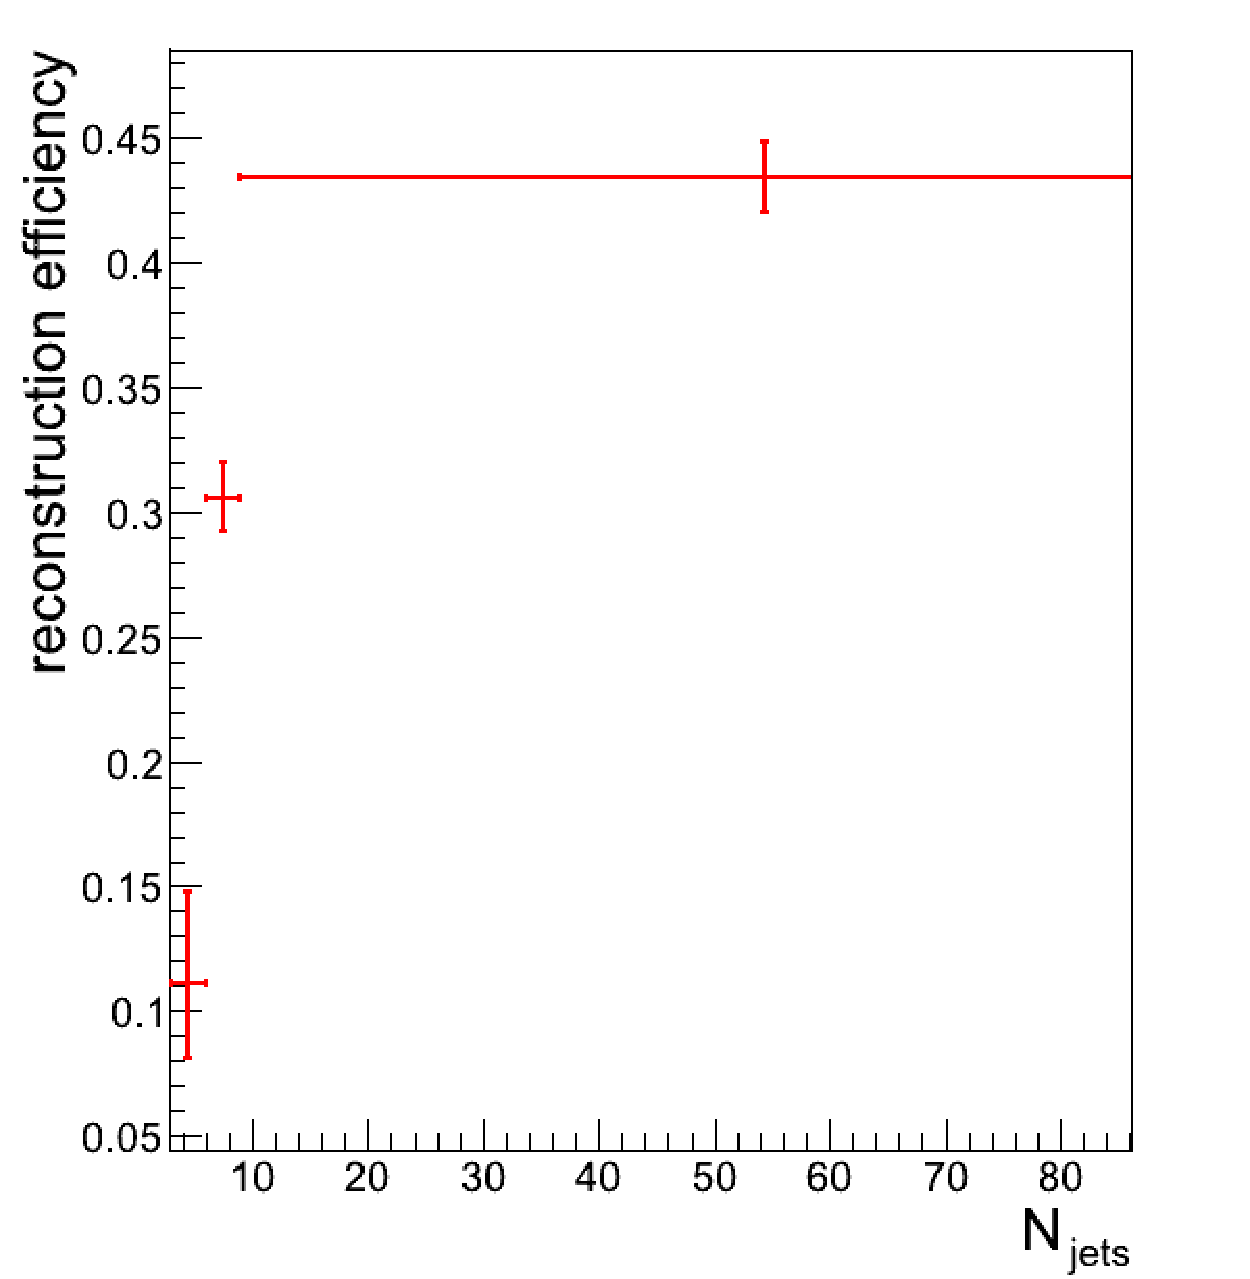
\includegraphics[width=0.3\textwidth]{figs/topNjet.pdf}
    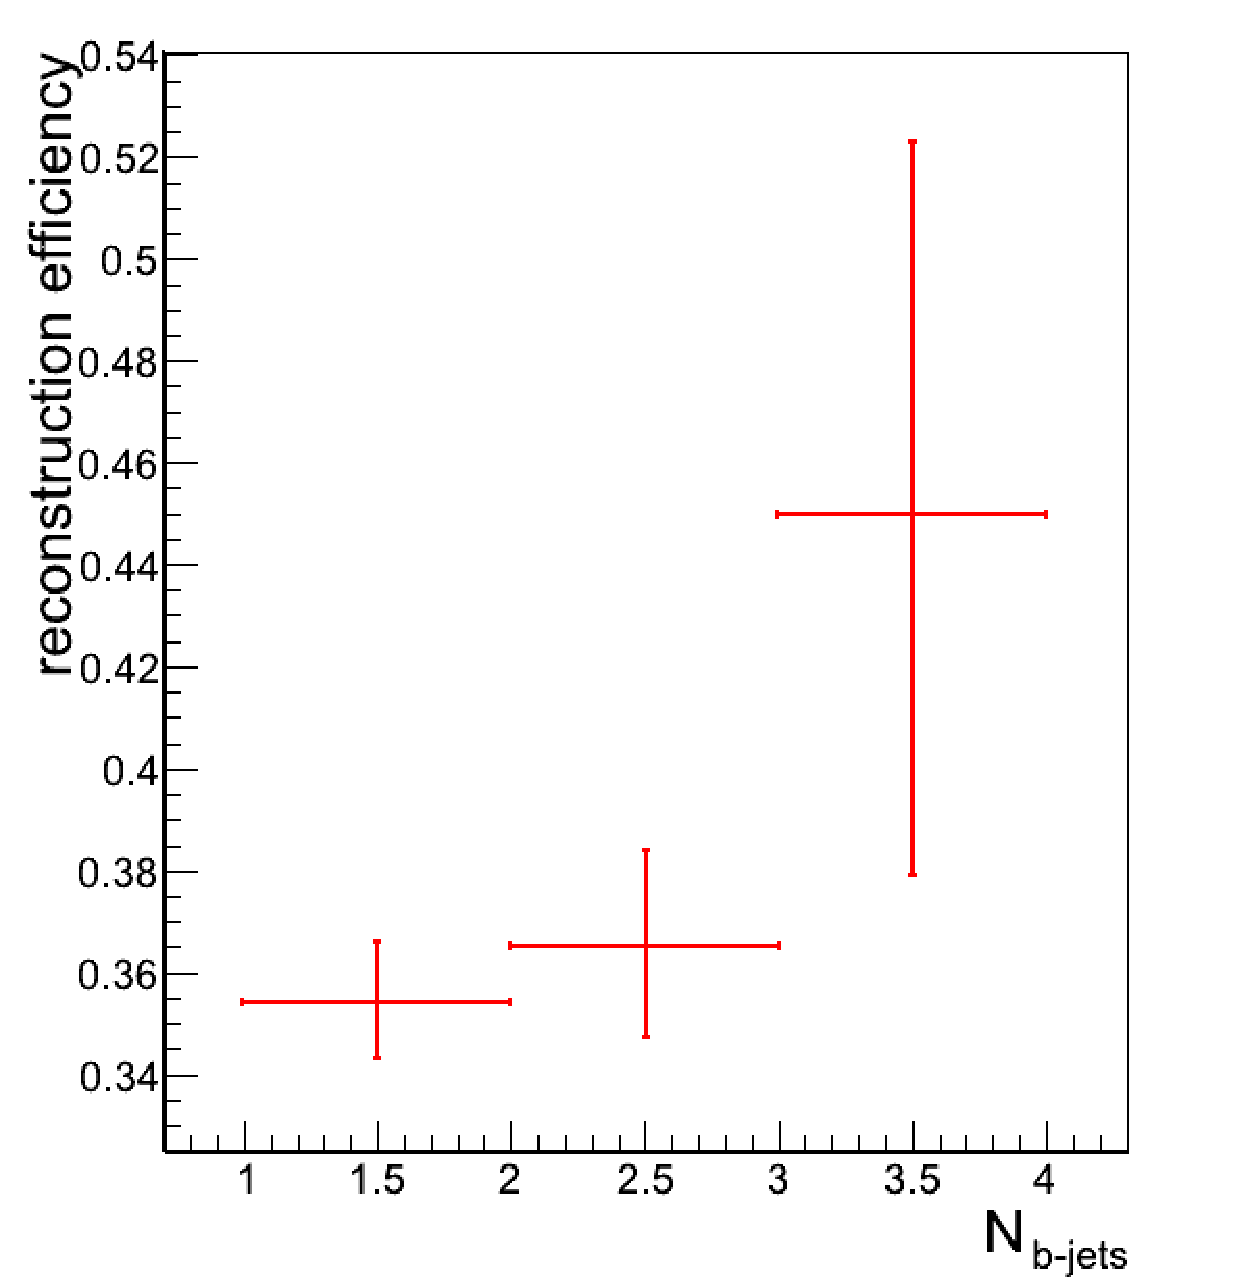
\includegraphics[width=0.3\textwidth]{figs/topNbjet.pdf} \\
    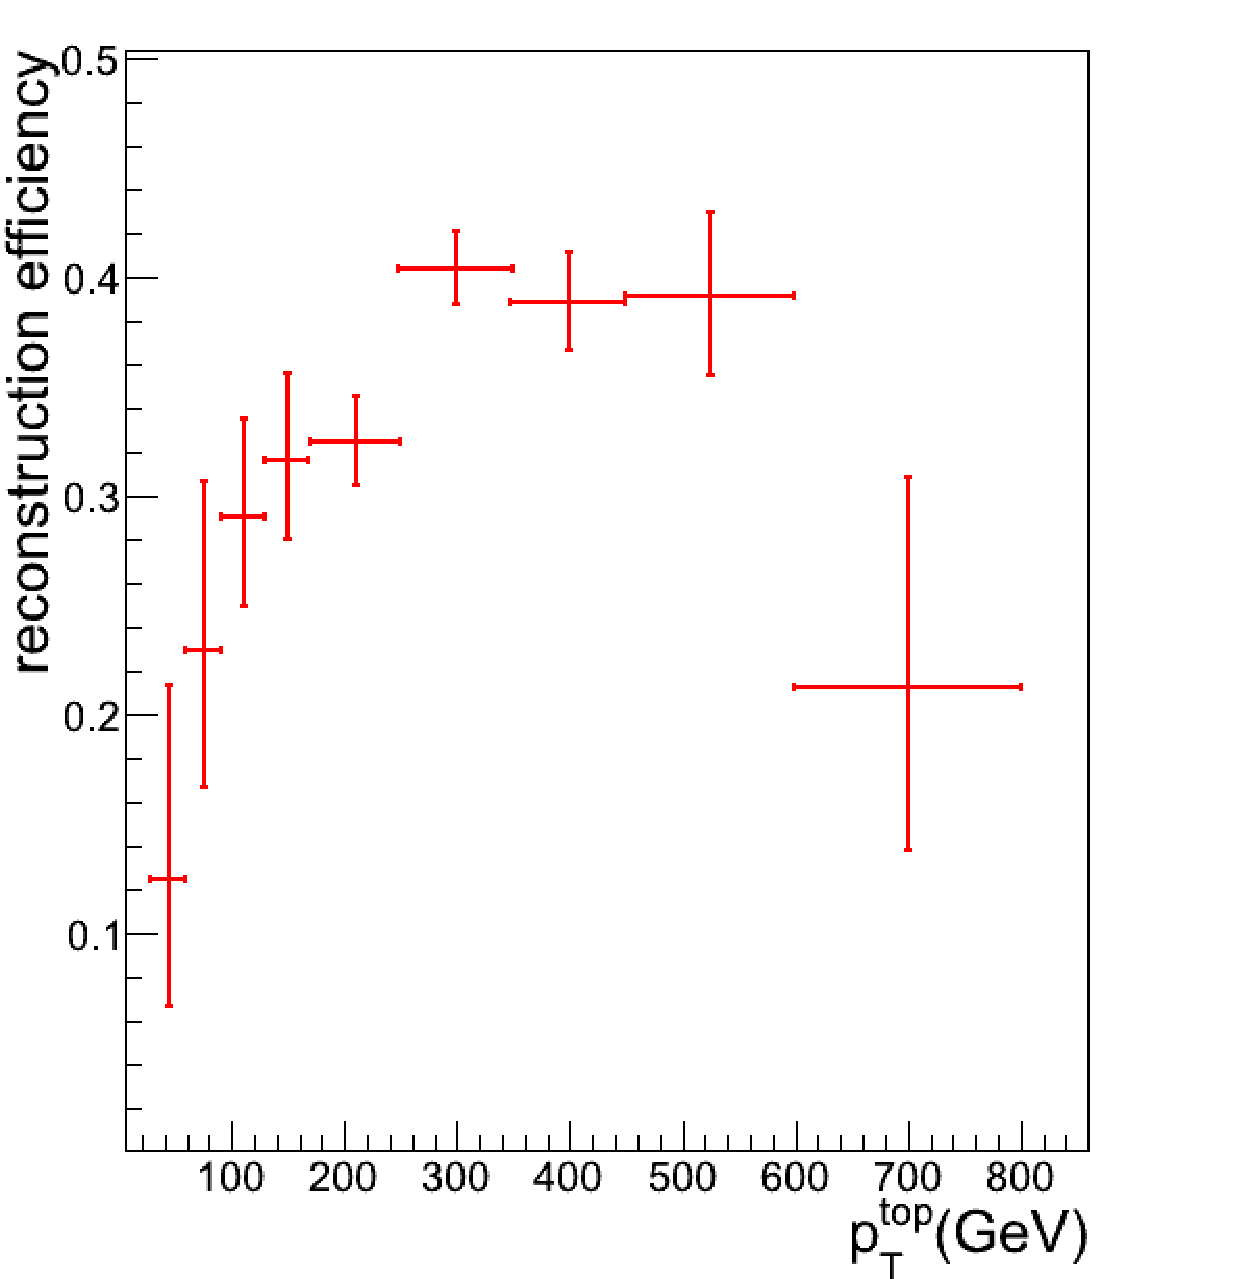
\includegraphics[width=0.3\textwidth]{figs/topPt.pdf}
    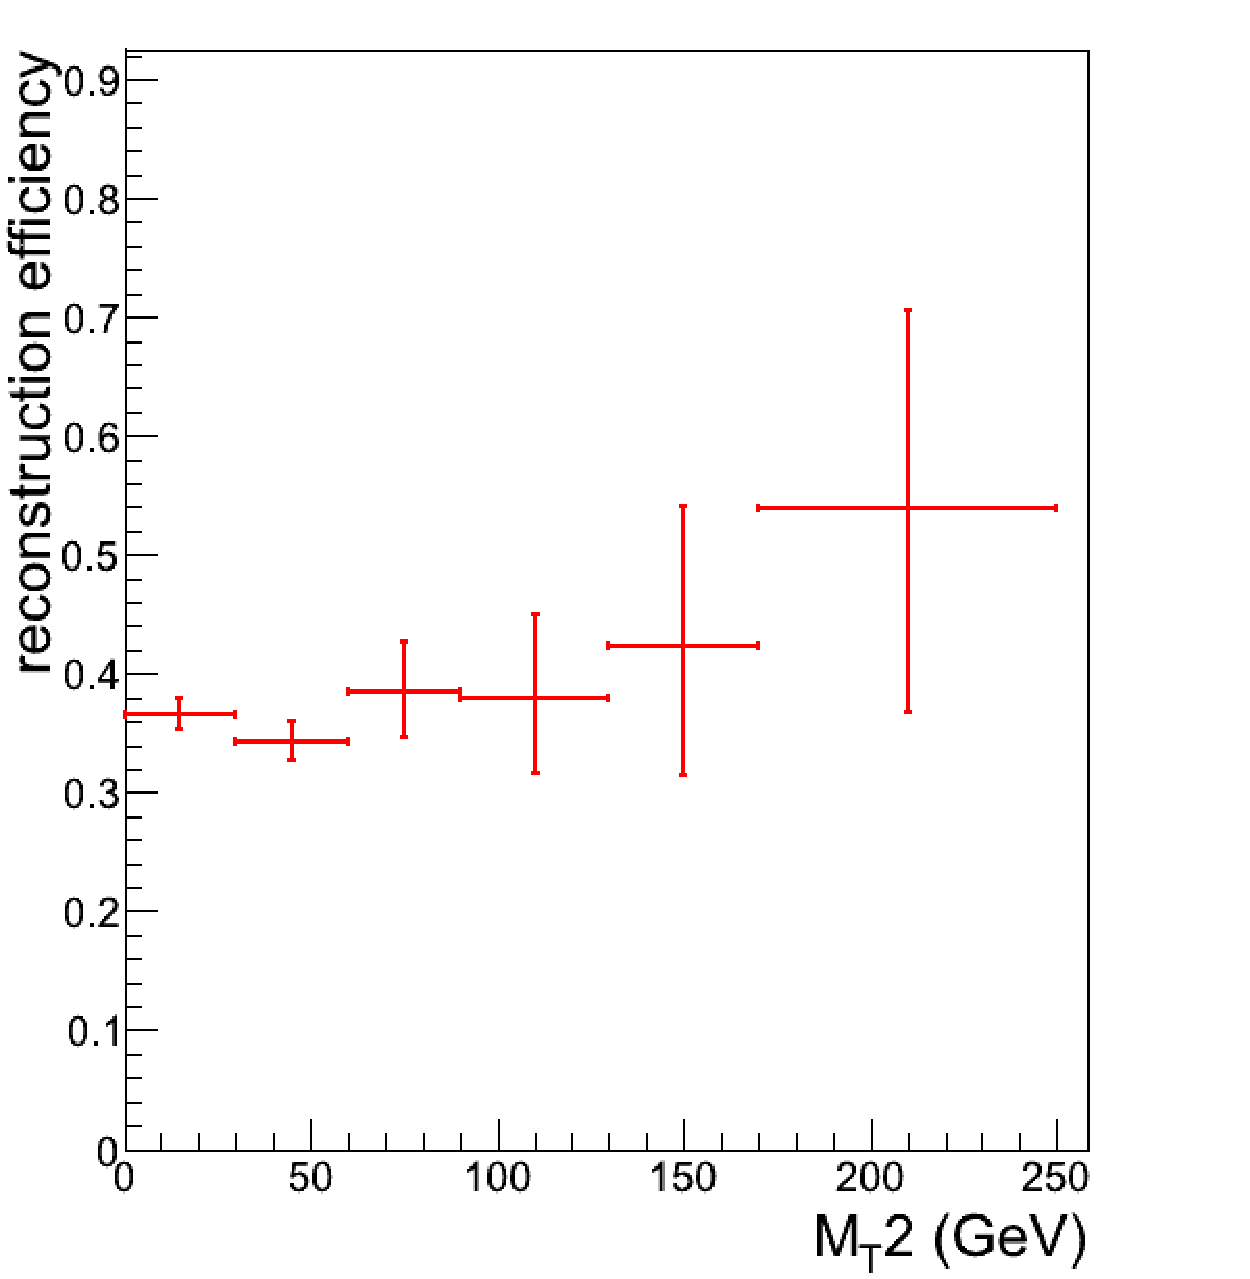
\includegraphics[width=0.3\textwidth]{figs/topMT2.pdf}
    \caption{The efficiency of top quark reconstruction algorithm is shown vs. number of jets (top-left) and number of
b-tagged jets (top-right), top $\pT$ (bottom-left) and $\mttwo$  and (bottom-right).}
    \label{figtopref_eff}
\end{figure}


The fake rate of the top reconstruction algorithm is also studied. Fake Rate, can be defined as the Probability of reconstructing top from each 3 jets in a $W$ + jets event. So the ratio is normalized to the number of jets. The results after applying all MT2b cuts on the WJetsToLNu-HT-400ToInf-8TeV sample are shown in Figure \ref{figtopref_fake}. The studies show that the fake rate value is around $20\%$.


\begin{figure}[htbp] 
\centering
    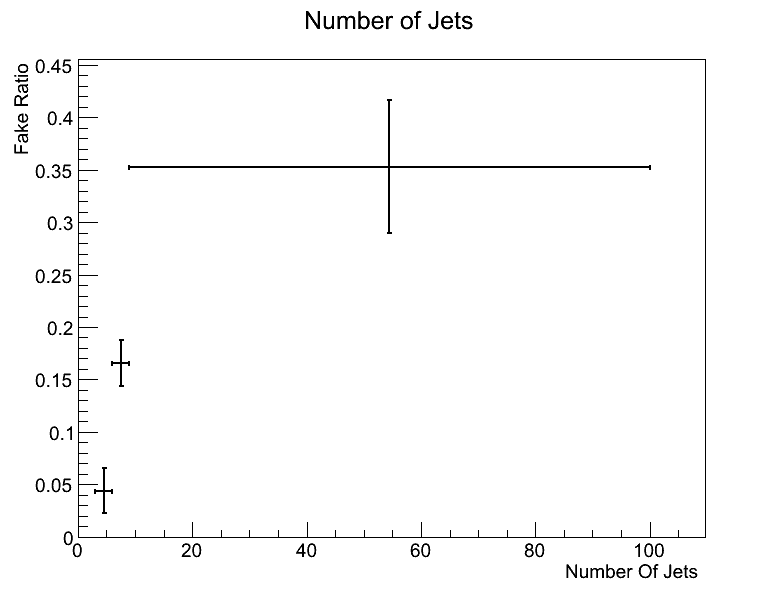
\includegraphics[width=0.3\textwidth]{figs/top_fake_NJets.png}
    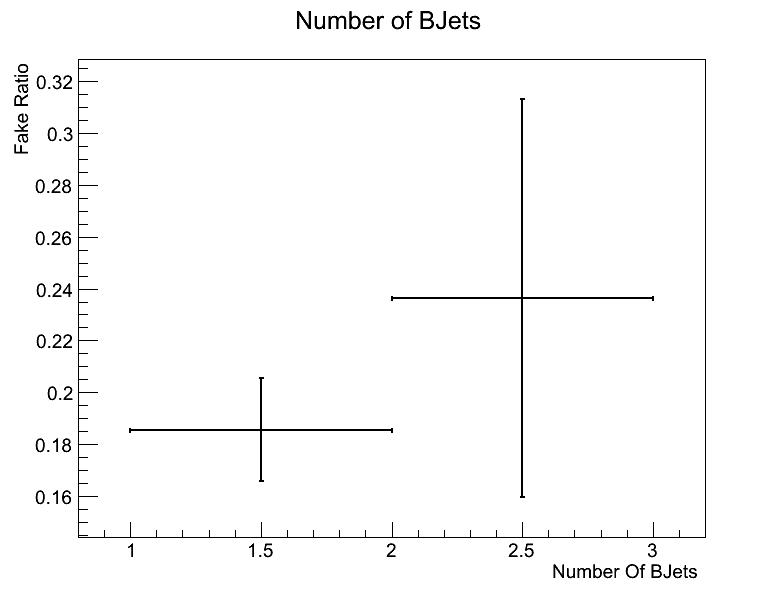
\includegraphics[width=0.3\textwidth]{figs/top_fake_NBJets.png} \\
    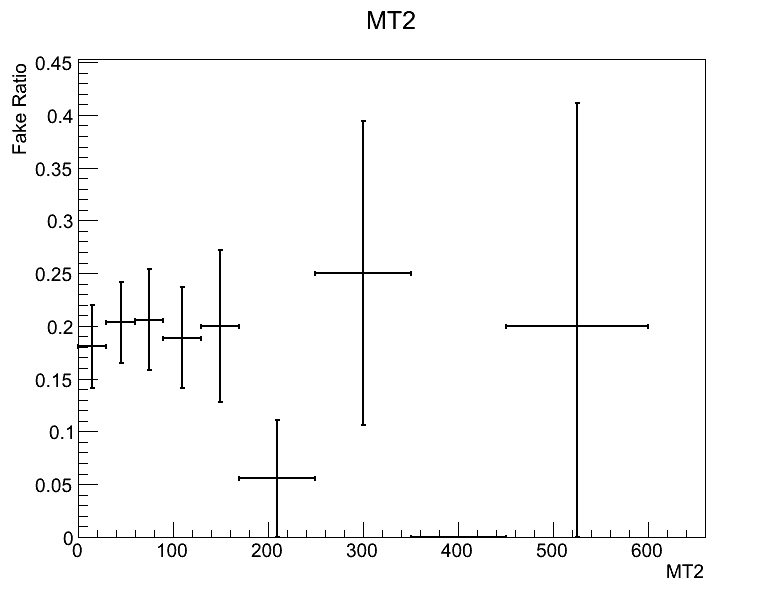
\includegraphics[width=0.3\textwidth]{figs/top_fake_MT2.png}
    \caption{The fake rate of the top reconstruction algorithm is shown vs. number of jets (top-left), number
of b-tagged jets (top-right) and $\mttwo$ (bottom).}
    \label{figtopref_fake}
\end{figure}

\section{Datasets and MC samples}
\label{sect:dataMC}
To reconstruct the objects, the CMSSW\_5\_3\_7\_patch5 is used for both data and Monte Carlo(MC).
The data used in this analysis corresponds to 18.1 \fbinv in \hadtau\hadtau channel and 19.6 \fbinv in $l\hadtau$ channel of proton-proton collisions in the center of mass energy of $\sqrt{s}$ = 8 TeV 
which was taken in 2012. The datasets used for $e\tau_{had}$, $\mu\tau_{had}$ and $\tau_{had}\tau_{had}$ channels, the run range and the corresponding integrated luminosities are mentioned Table ~\ref{Tab.DataSamples}.
\begin{table}[!Hhtb]

\begin{center}
\small{
\begin{tabular}{|l|c|c|}
\hline
Dataset Name & Run--range & Luminosity(\fbinv) \\
\hline
\multicolumn{3}{|c|}{$e\tau_{had}$ and $\mu\tau_{had}$ channels} \\
\hline
/TauPlusX/Run2012A-22Jan2013-v1/AOD   & 190456--193621 & 0.887\\
/TauPlusX/Run2012B-22Jan2013-v1/AOD   & 193833--196531 & 4.446\\
/TauPlusX/Run2012C-22Jan2013-v1/AOD   & 198022--203742 & 7.153\\
/TauPlusX/Run2012D-22Jan2013-v1/AOD   & 203777--208686 & 7.318\\
\hline
\multicolumn{3}{|c|}{$\tau_{had}\tau_{had}$ channel} \\
\hline
/Tau/Run2012A-22Jan2013-v1/AOD   & 190456--193621 & 0.887 \\
/TauParked/Run2012B-22Jan2013-v1/AOD & 193833--196531 & 4.446 \\
/TauParked/Run2012C-22Jan2013-v1/AOD & 198022--203742 & 7.153 \\
/TauParked/Run2012D-22Jan2013-v1/AOD & 203777--208686 & 7.318 \\
\hline

\end{tabular}
}
\end{center}
\caption{
  List of datasets analysed by different channels.
}
\label{Tab.DataSamples}
\end{table}

For data the golden JSON file,{\small Cert\_190456-208686\_8TeV\_22Jan2013ReReco\_Collisions12\_JSON.txt} is used and it can be found in Table.~\ref{Tab.Triggers} the list of trigger paths which is used for this analysis data. 
\begin{table}[!Hhtb]
\small{
\begin{center}
\begin{tabular}{|l|c|c|}
\hline
HLT Path   & L1 Seed  & Luminosity(\fbinv) \\
\hline
\multicolumn{3}{|c|}{$e\tau_{had}$ channel} \\
\hline
Ele20\_CaloIdVT\_CaloIsoRhoT\_TrkIdT\_TrkIsoT\_LooseIsoPFTau20 & $^{1}$                 &  $0.7$    \\
Ele22\_eta2p1\_WP90Rho\_LooseIsoPFTau20                        & $^{2}$                 & $18.7$    \\   
\hline
\multicolumn{3}{|c|}{$mu\tau_{had}$ channel} \\
\hline
IsoMu18\_eta2p1\_LooseIsoPFTau20                               &    SingleMu16er        &  $0.7$  \\
IsoMu17\_eta2p1\_LooseIsoPFTau20                               &    SingleMu14er        & $18.7$  \\
\hline
\multicolumn{3}{|c|}{$\tau_{had}\tau_{had}$ channel} \\
\hline
DoubleMediumIsoPFTau35\_Trk5\_eta2p1                          &  $^{3}$                       & $3.9$ \\
DoubleMediumIsoPFTau35\_Trk1\_eta2p1                          &  $^{3}$                       & $14.2$ \\
\hline
\end{tabular}
\end{center}
$^{1}$ SingleIsoEG18er or SingleEG20 \\
$^{2}$ SingleIsoEG18er or SingleIsoEG20er or SingleEG22 \\
$^{3}$ L1\_DoubleTauJet44er or L1\_DoubleJetC64 \\
}
\caption{
  Trigger paths used by $e\tau_{had}$, $\mu\tau_{had}$ and $\tau_{had}\tau_{had}$ channels
  for $2012$ data. All the paths given in the table remained unprescaled during the whole and $2012$ data--taking period.
}
\label{Tab.Triggers}
\end{table}
MC samples are used for different standard model backgrounds and signals. These samples are officially generated and reconstructed by the CMS collaboration. The full list of the MC samples and their cross sections are given in Table ~\ref{Tab.MCSamples}. For most of the samples the most accurate calculation of the cross sections available in the literature (usually NLO and NNLO) are used. 
\begin{table}[!Hhtb]
\begin{center}
\small{
\begin{tabular}{|l|c|}
\hline
\multicolumn{2}{|c|}{MC samples } \\
\hline
%Dataset Description                &   
Dataset Name                                            & Cross-Section (pb)    \\
\hline
\multicolumn{2}{|c|}{QCD used in $e/\mu\tau_{had}$ channels }\\
\hline
%QCD BCtoE                        &    
/QCD\_Pt\_20...inf\_BCtoE\_TuneZ2star\_8TeV\_pythia6                & Ref. ~\cite{Prep}\\ 
%QCD EM\_Enriched                 &    
%/QCD\_Pt\_20...inf\_EMEnriched\_TuneZ2star\_8TeV\_pythia6           & Ref. ~\cite{Prep}\\
%QCD Mu\_Enriched                 &
/QCD\_Pt-15...inf\_MuEnrichedPt5\_TuneZ2star\_8TeV\_pythia6         & Ref. ~\cite{Prep}\\
%$\gamma$+jets                       &
/GJets\_HT-40...inf\_8TeV-madgraph                                  & Ref. ~\cite{Prep}\\
\hline
\multicolumn{2}{|c|}{QCD used in $\tau_{had}\tau_{had}$ channel }\\
\hline
%QCD                                &   
/QCD\_HT-100...inf\_TuneZ2star\_8TeV-madgraph-pythia6            &\\
\hline

\multicolumn{2}{|c|}{Top }\\
\hline
%Single top (tW)                    &   
/T\_tW-channel-DR\_TuneZ2star\_8TeV-powheg-tauola       & $22.4$                \\
%Single anti-top ($\bar{\rm t}$W)   &   
/Tbar\_tW-channel-DR\_TuneZ2star\_8TeV-powheg-tauola    & $22.4$\\
%Single top ($s$-channel)           &   
/T\_s-channel\_TuneZ2star\_8TeV-powheg-tauola           & $3.8$\\%3.79
%Single anti-top ($s$-channel)      &   
/Tbar\_s-channel\_TuneZ2star\_8TeV-powheg-tauola        & $1.8$\\%1.76
%Single top ($t$-channel)           &   
/T\_t-channel\_TuneZ2star\_8TeV-powheg-tauola           & $56.4$\\
%Single anti-top ($t$-channel)      &   
/Tbar\_t-channel\_TuneZ2star\_8TeV-powheg-tauola        & $30.7$\\

%$\ttbar$                           & 
/TTJets\_MassiveBinDECAYTTJets\_TuneZ2star\_8TeV  &  $245.8$       \\
-madgraph-tauola                                        &               \\
%$\ttbar$+$\gamma$+ jets              &
/TTGJets\_8TeV-madgraph                                  &  $2.2$              \\%2.166
%$\ttbar$\,+\,Higgs + jets              &
/TTH\_Inclusive\_M-125\_8TeV\_pythia6                    &  $0.1$               \\
%$\ttbar$\,+\,W + jets                  &
/TTWJets\_8TeV-madgraph                                  &  $0.2$              \\
%$\ttbar$\,+\,Z + jets                  &
/TTZJets\_8TeV-madgraph                                  &  $0.2$                \\
%$\ttbar$\,+\,WW + jets                 &
/TTWWJets\_8TeV-madgraph                                 &  $0.002$\\%$2\times 10^{-3}$                \\

\hline
\multicolumn{2}{|c|}{$ZX$ }\\
\hline
%Z $\rightarrow \ell\ell$                 &
/DYJetsToLL\_M-10To50filter\_8TeV-madgraph-tarball      &   $876.8$               \\
%Z $\rightarrow \ell\ell$                &  
/DYJetsToLL\_M-50\_TuneZ2Star\_8TeV-madgraph-tarball    &   $3503.7$               \\
%Z + 1 jet                           &   
/DY1JetsToLL\_M-50\_TuneZ2Star\_8TeV-madgraph           &   $666.3$               \\
%Z + 2 jets                          &   
/DY2JetsToLL\_M-50\_TuneZ2Star\_8TeV-madgraph           &   $215.0$               \\
%Z + 3 jets                          &   
/DY3JetsToLL\_M-50\_TuneZ2Star\_8TeV-madgraph           &   $60.7$               \\
%Z + 4 jets                          &   
/DY4JetsToLL\_M-50\_TuneZ2Star\_8TeV-madgraph           &   $27.3$               \\
%WZ                                 &   
/WZJetsTo3LNu\_TuneZ2\_8TeV-madgraph-tauola             &  $1.1$                \\
%WZ                                 &   
/WZJetsTo2L2Q\_TuneZ2star\_8TeV-madgraph-tauola         &  $2.2$                \\
%ZZ                                 &   
/ZZJetsTo4L\_TuneZ2star\_8TeV-madgraph-tauola           &  $0.2$                \\
%ZZ                                 &   
/ZZJetsTo2L2Nu\_TuneZ2star\_8TeV-madgraph-tauola        &  $0.7$                \\
%ZZ                                 &   
/ZZJetsTo2L2Q\_TuneZ2star\_8TeV-madgraph-tauola         &  $2.5$                \\
\hline
\multicolumn{2}{|c|}{W}\\
\hline

%W + jets                           &   
/WJetsToLNu\_TuneZ2Star\_8TeV-madgraph-tarball          &  $36257.2$              \\
%W + 1 jet                           &   
/W2JetsToLNu\_TuneZ2Star\_8TeV-madgraph-tarball         &  $6381.2$               \\
%W + 2 jets                          &   
/W2JetsToLNu\_TuneZ2Star\_8TeV-madgraph-tarball         &  $2039.8$               \\
%W + 3 jets                          &   
/W3JetsToLNu\_TuneZ2Star\_8TeV-madgraph-tarball         &  $612.5$               \\
%W + 4 jets                          &   
/W4JetsToLNu\_TuneZ2Star\_8TeV-madgraph-tarball         &  $251.0$                \\
\hline
\multicolumn{2}{|c|}{WW}\\
\hline
%WW                                 &   
/WWJetsTo2L2Nu\_TuneZ2star\_8TeV-madgraph-tauola        &  $5.8$                \\

\hline
\multicolumn{2}{|c|}{Higgs}\\
\hline
%WW                                 &   
/GluGluToHToTauTau\_M-125\_8TeV-powheg-pythia6          &  $1.2$                \\
/VBF\_HToTauTau\_M-125\_8TeV-powheg-pythia6             &  $0.1$                \\
/WH\_ZH\_TTH\_HToTauTau\_M-125\_8TeV-pythia6-tauola     &  $0.08$\\
%$$8\times10^{-2}$                \\

\hline

\end{tabular}
}
\end{center}

\caption{List of MC samples used as backgrounds produced in /Summer12-DR53X-PU\_S10\_START53\_*/AODSIM scenario.}
\label{Tab.MCSamples}
\end{table}

The investigated SUSY signal in this analysis is {\small $pp \rightarrow \chip \chim \rightarrow \tau^+ \tau^- \MET$} called {\small "TChipChimSlepSnu"} produced with \PYTHIA $6.0$ at the level of LHE. \TAUOLA is used to decay precisely the produced $\tau$'s, then the generated events are
passed through the CMS official Fast-Sim process.


\section{Physics Object Definition}
\label{sect:objdef}
To define the physics objects of the analysis, we follow the recommendations and selections of another CMS analysis which search for Higgs bosons decaying to $\tau$ pairs \cite{CMS_AN_2013-188}. Due to the very similar final states, it is well motivated to avoid duplication of the efforts to define and optimize the object selections. For the completeness of the note, the object selections are reviewed shortly here. More detail can be found in \cite{CMS_AN_2013-188} and \cite{HiggsTauTautwiki}

\subsection{Electron}
Electron identification is based on a MVA (Boosted Decision Tree) method ~\cite{Hocker:2007ht} which also cleans the colletion of electron from jet\,$\rightarrow e$  fakes. The training process takes advantage of two bins of $\pt$ and three bins of $\eta$, running over a sample of $Z \rightarrow ee$  events selected in data. Those oppositely charged electrons pair closest to Z-boson peak mass is taken as "signal" and the other electron candidates as "background". The training input variables are described in ~\cite{CMS_AN_2013-188}. Different discriminators are trained on electrons passing the criteria of single electron trigger and also on non triggered electrons. In this analysis the latter case is chosen.   
Depending on the BDT output, a loose and tight working point of \textit{ElIDMVANoTrig} algorithm can be defined. The citeria in different bins of $\pt$ and $\eta$ are given in Table ~\ref{Tab.electronMVAIDwp}.

\begin{table}[!h]
\begin{center}
\begin{tabular}{|l|l|c|c|}
\hline\hline
\multicolumn{2}{|c|}{Kinematic range}                & Loose & Tight \\
\hline\hline
\multirow{3}{*}{$\pt < 20$~\GeV} & $\vert \eta \vert < 0.8$         & 0.925 & 0.925 \\
                  & $0.8 < \vert \eta \vert < 1.479$ & 0.915 & 0.915 \\
                  & $\vert \eta \vert > 1.479$       & 0.965 & 0.965 \\\hline
\multirow{3}{*}{$\pt > 20$~\GeV} & $\vert \eta \vert < 0.8$         & 0.905 & 0.925 \\
                  & $0.8 < \vert \eta \vert < 1.479$ & 0.955 & 0.975 \\
                  & $\vert \eta \vert > 1.479$       & 0.975 & 0.985 \\
\hline\hline
\end{tabular}
\end{center}
\caption{
  Discriminator thresholds for the Loose and Tight MVA electron identification working--points respectively.
}
\label{Tab.electronMVAIDwp}
\end{table}     

To reject those electrons which is coming from photon conversions, it is required that the electron touches all layers of Pixel detector. Furthermore if there is an oppositely charged track near electron which is fitted to a common vertex inside of tracker volume that electron is rejected.  
\subsection{Muon}
Muons are required to be reconstructed by the Tracker or the Global muon reconstruction algorithm and to be identified as 
muons by tight particle flow algorithm.

The particle flow algorithm identifies  muons by applying several criteria.

$\bullet$ The number of pixel hit(s) associated to muon track\,$\geq $\,1

$\bullet$ Number of tracker layers with hits should be $\geq $\,6

$\bullet$ The number of hits in muon system $\geq $\,1

$\bullet$ Tracker track matched with at least one muon segment (in any station)

$\bullet$ $\chi ^{2}/{\rm NDF} $ for the global track fit\,$< $\,10 ,

$\bullet$ Impact parameter constrains between the muon track and the selected primary vertex 
 $d_{z} < $\,0.5 cm and $d_{0} <$\,0.2 cm.

\subsection{Muon and electron isolation}

In order to reduce the background contributions from QCD multi–jet events, electrons and
muons are required to be isolated. The isolation is computed as the $\pt$ sum of charged particles (including charged hadrons, 
electrons and muons), neutral hadrons plus photons reconstructed by the PF algorithm within a cone of size
$\Delta R_{\rm iso}$ = 0.4 (0.3) around the direction of the muon (electron). 
In the innermost region
(``veto cone'') neutral
hadrons and photons  are excluded from the computation of the isolation $\pt$ sum in order to prevent energy deposits in the electromagnetic and hadronic calorimeters. Charged particles close to the direction of electrons  are excluded too in order to avoid tracks due to conversions of photons emitted by Bremsstrahlung processes to spoil the isolation.

For the lepton isolation the photon and neutral hadron candidates are required to have a transverse energy of $\pt>0.5\,\GeV$. This reduces pile-up effects. The correction of pile-up to isolation is done by applying $\Delta\beta$ corrections.
\begin{linenomath}
\begin{equation}
\label{eq:muonisolation1}
I_{e/ \mu}\,=\,\Sigma\, \pt^{\rm charged }(\Delta z <2\,mm)+max(\pt^{\rm photon}+\pt^{h0 }-\Delta \beta,0),
\end{equation}
\end{linenomath}
The $\Delta\beta$ corrections are computed by summing the transverse momenta of charged particles
that have longitudinal impact parameters $\Delta z > 2$ mm with respect to the lepton production
vertex and scaling the sum by a factor 0.5:
\begin{linenomath}
\begin{equation}
\label{eq:muonisolation2}
\Delta\beta\,=\,0.5\, \Sigma \pt^{\rm charged }(\Delta z > 2mm).
\end{equation}
\end{linenomath}

\subsection{\texorpdfstring{Hadronic $\tau$}{Hadronic tau}} 
\label{sec:hadTau}
The "Hadron plus Strip" (HPS) algorithm~\cite{2012JInst...7.1001C} is employed to reconstruct the hadronic decays of $\tau$ leptons with the jet constituents as input. The algorithm is seeded by PF jets reconstructed using the anti-$k_{\rm T}$ procedure with a distance parameter of $R=0.5$. To discriminate against quark and gluon jets, jets with extra particles not compatible with the hadronic $\tau$ decays are rejected. Additional criteria are used to suppress the contributions from electrons and muons in the hadronic $\tau$ ($\hadtau$) collection.

Based on the expected particles in the final state of the hadronic $\tau$ decay, different combinations of charged hadrons and $\pi^0$ candidates are considered. The $\pi^0 (\to\gamma\gamma)$ candidates are reconstructed using PF photons with $\pt>2.5\,\GeV$, falling into $\eta-\phi$ "strips" with specific size~\cite{CMS_AN_2013-171}. While a \textbf{single charged hadron} is an indication of $\tau^{\pm}\to\pi^{\pm}\nu_{\tau}$, a combination of \textbf{three charged hadrons} fulfilling a set of requirements are considered as the process of $\tau^{\pm}\to a_1^{\pm}\nu_{\tau}\to\pi^{\pm}\pi^{\mp}\pi^{\pm}\nu_{\tau}$. \textbf{One charged hadron plus two Strips} with a dedicated selection is assigned to $\tau^{\pm}\to a_1^{\pm}\nu_{\tau}\to\pi^{\pm}\pi^{0}\pi^{0}\nu_{\tau}$ decays. Finally the signature of  $\tau^{\pm}\to\rho^{\pm}\nu_{\tau}\to\pi^{\pm}\pi^{0}\nu_{\tau}$ decay is searched for in \textbf{one charged hadron plus one Strip} combinations. All charged hadrons and strips in the $\tau$ decay mode reconstruction must be within a narrow cone around the jet axis where the cone size depends on the $\tau$ jet $\pt$. Details on specific selections for each category as well as the $\pt$ dependence of the cone size can be found in Ref.~\cite{CMS_AN_2013-171}

The isolation variable is defined as the sum of the $\pt$ of charged hadrons and the $\et$ of photons within a cone of $\Delta R = 0.5$ around the $\hadtau$ axis. Particles used to reconstruct the $\hadtau$ candidate are excluded. The contribution of pile-up to the $\Tau$ isolation is accounted for by applying the so-called $\Delta\beta$ corrections. The selection criteria for charged hadrons in the isolation sum together with the pile-up subtraction procedure can be found in Ref.~\cite{CMS_AN_2013-171}. The Loose, Medium and Tight working points of {\it CombinedIsoDBSumPtCorr3Hits} algorithm correspond to isolation variables less than 2.0, 1.0 and 0.8\,$\GeV$, respectively.

The $\hadtau$ candidates are vetoed if signals exist in the muon system close to the $\hadtau$ direction. Loose, Medium and Tight working points are provided, corresponding to different $\hadtau$ identification efficiencies and $\mu\to\hadtau$ fake rates~\cite{CMS_AN_2013-171}. To discriminate against electrons i.e., rejecting $e\to\hadtau$ fakes, a multivariate discriminator is trained for which the Loose, Medium, Tight and very-Tight working points are defined based on the outputs of 16 different BDT's. Each BDT is associated to a category of $\hadtau$ candidates where the classification of $\hadtau$'s is performed according to their kinematics and decay mode as well as their closeness to a GSF electron. The working points are optimized to achieve the lowest $e\to\tau$ rate possible with a given $\hadtau$ identification efficiency~\cite{CMS_AN_2012-417}.

%Tau leptons from Higgs boson decays are expected to be isolated in the detector, while leptons from heavy-flavor (c and b) decays and decays in flight are expected to be found inside jets. A measure of isolation is used to discriminate the signal from the QCD multijet background, based on the charged hadrons, photons, and neutral hadrons falling within a cone around the lepton momentum direction.
%Electron, muon, and tau lepton isolation are estimated as
%\begin{equation}\begin{aligned}
%I_{\Pe,\Pgm} &=  \sum_{\rm charged}  \pt + \text{max}\left( 0, \sum_{\rm neutral}  \pt
%                                        +  \sum_{\gamma} {\pt} - 0.5 \sum_{\rm charged, pileup} \pt  \right ), \\
%I_{\Tau} &=  \sum_{\rm charged}  \pt + \text{max}\left( 0, \sum_{\gamma} {\pt} - 0.46 \sum_{\rm charged, pileup} \pt  \right ),
%\label{eq:reconstruction_isolation}
%\end{aligned}\end{equation}
%where $\sum_\text{charged}\pt$ is the scalar sum of the transverse momenta of the charged hadrons, electrons, and muons from the primary vertex located in a cone centered around the lepton direction of size $\Delta R = \sqrt{(\Delta\eta)^2+(\Delta\phi)^2}$ of 0.4 for electrons and muons and 0.5 for tau leptons.
%The sums $\sum_\text{neutral}\pt$ and $\sum_{\gamma} \pt$ represent the same quantities for neutral hadrons and photons, respectively. In the case of electrons and muons the innermost region is excluded
%to avoid the footprint in the calorimeter of the lepton itself from entering the sum.
%Charged particles close to the direction of the electrons are excluded as well, to prevent tracks originating from the conversion of photons emitted by the bremsstrahlung process from spoiling the isolation. In the case of \Tau, the particles used in the reconstruction of the lepton are excluded. The contribution of pileup photons and neutral hadrons
%is estimated from the scalar sum of the transverse momenta of charged hadrons from pileup vertices in the isolation cone $\sum_\text{charged, pileup}$. This sum is multiplied by a factor of 0.5 that approximately corresponds to the ratio of neutral-to-charged hadron production in the hadronization process of inelastic $\Pp\Pp$ collisions. In the case of \Tau, a value of 0.46 is used, as the neutral hadron contribution is not used in the computation of $I_{\tauh}$. An $\eta$, \pt, and lepton-flavor dependent threshold on the isolation variable is applied.


\subsection{Jet and MET reconstruction}
\label{sec:jetmet}
Particle flow algorithm is used to reconstruct jets and \ETmiss. The medium working point of the Combined Secondary Vertex algorithm is used to tag bjets.

The minimum $\Delta\phi$ between \ETmiss and jets, hereafter referred to as \mindphifour, is used in this analysis to suppress QCD events. To calculate \mindphifour, all the pf-jets in $|\eta|<5.0$ region and with $\pt>40\GeV$ are used without applying any extra identification. $\mindphifour > 1.0$ is found useful for this analysis.


\section{Trigger}
\label{sect:trigger}
\subsection{Trigger Study}
\label{sect:triggerstudy}

To have the best reach, two sets of triggers are compared. Their names and run ranges are shown in 
table \ref{Tab.TriggerPaths}. The corresponding prescaled triggers which are used to find the trigger plateau are also shown.

\begin{table}[!htb]
\begin{center}
\caption{On line triggers, their references and run ranges. A logical OR between SixJet and QuadJet is used.}
\label{Tab.TriggerPaths}
\begin{tabular}{|l|l|c|}
\hline
\multicolumn{3}{|c|}{HT}\\
\hline
Trigger Path & Prescaled Trigger & Run Range \\\hline
HLT\_PFHT650\_v5 & HLT\_PFHT350\_v3 & 190650-190750\\
HLT\_PFHT650\_v6 & HLT\_PFHT350\_v4 & 191000-191400\\ 
HLT\_PFHT650\_v7 & HLT\_PFHT350\_v5 & 191500-193750\\ 
HLT\_PFHT650\_v8 & HLT\_PFHT350\_v6 & 193750-196030\\ 
HLT\_PFHT650\_v9 & HLT\_PFHT350\_v7 & 196046-196531\\ 
\hline
\multicolumn{3}{|c|}{MultiJet}\\
\hline
HLT\_SixJet45\_v1  & HLT\_SixJet35\_v1  & 190640-190740\\
HLT\_SixJet45\_v2  & HLT\_SixJet35\_v2  & 191000-196030\\
HLT\_SixJet45\_v3  & HLT\_SixJet35\_v3  & 196040-196531\\
HLT\_QuadJet80\_v1 & HLT\_QuadJet70\_v1 & 190640-190740\\
HLT\_QuadJet80\_v2 & HLT\_QuadJet70\_v2 & 191000-196030\\
HLT\_QuadJet80\_v3 & HLT\_QuadJet70\_v3 & 196040-196531\\
\hline
\end{tabular}
\end{center}
\end{table}

To take into account the statistics (the peak of the selected events by the un-prescaled trigger figure \ref{fig.TriggerPlateau} (middle)),
\begin{figure}[!htb]
\centering
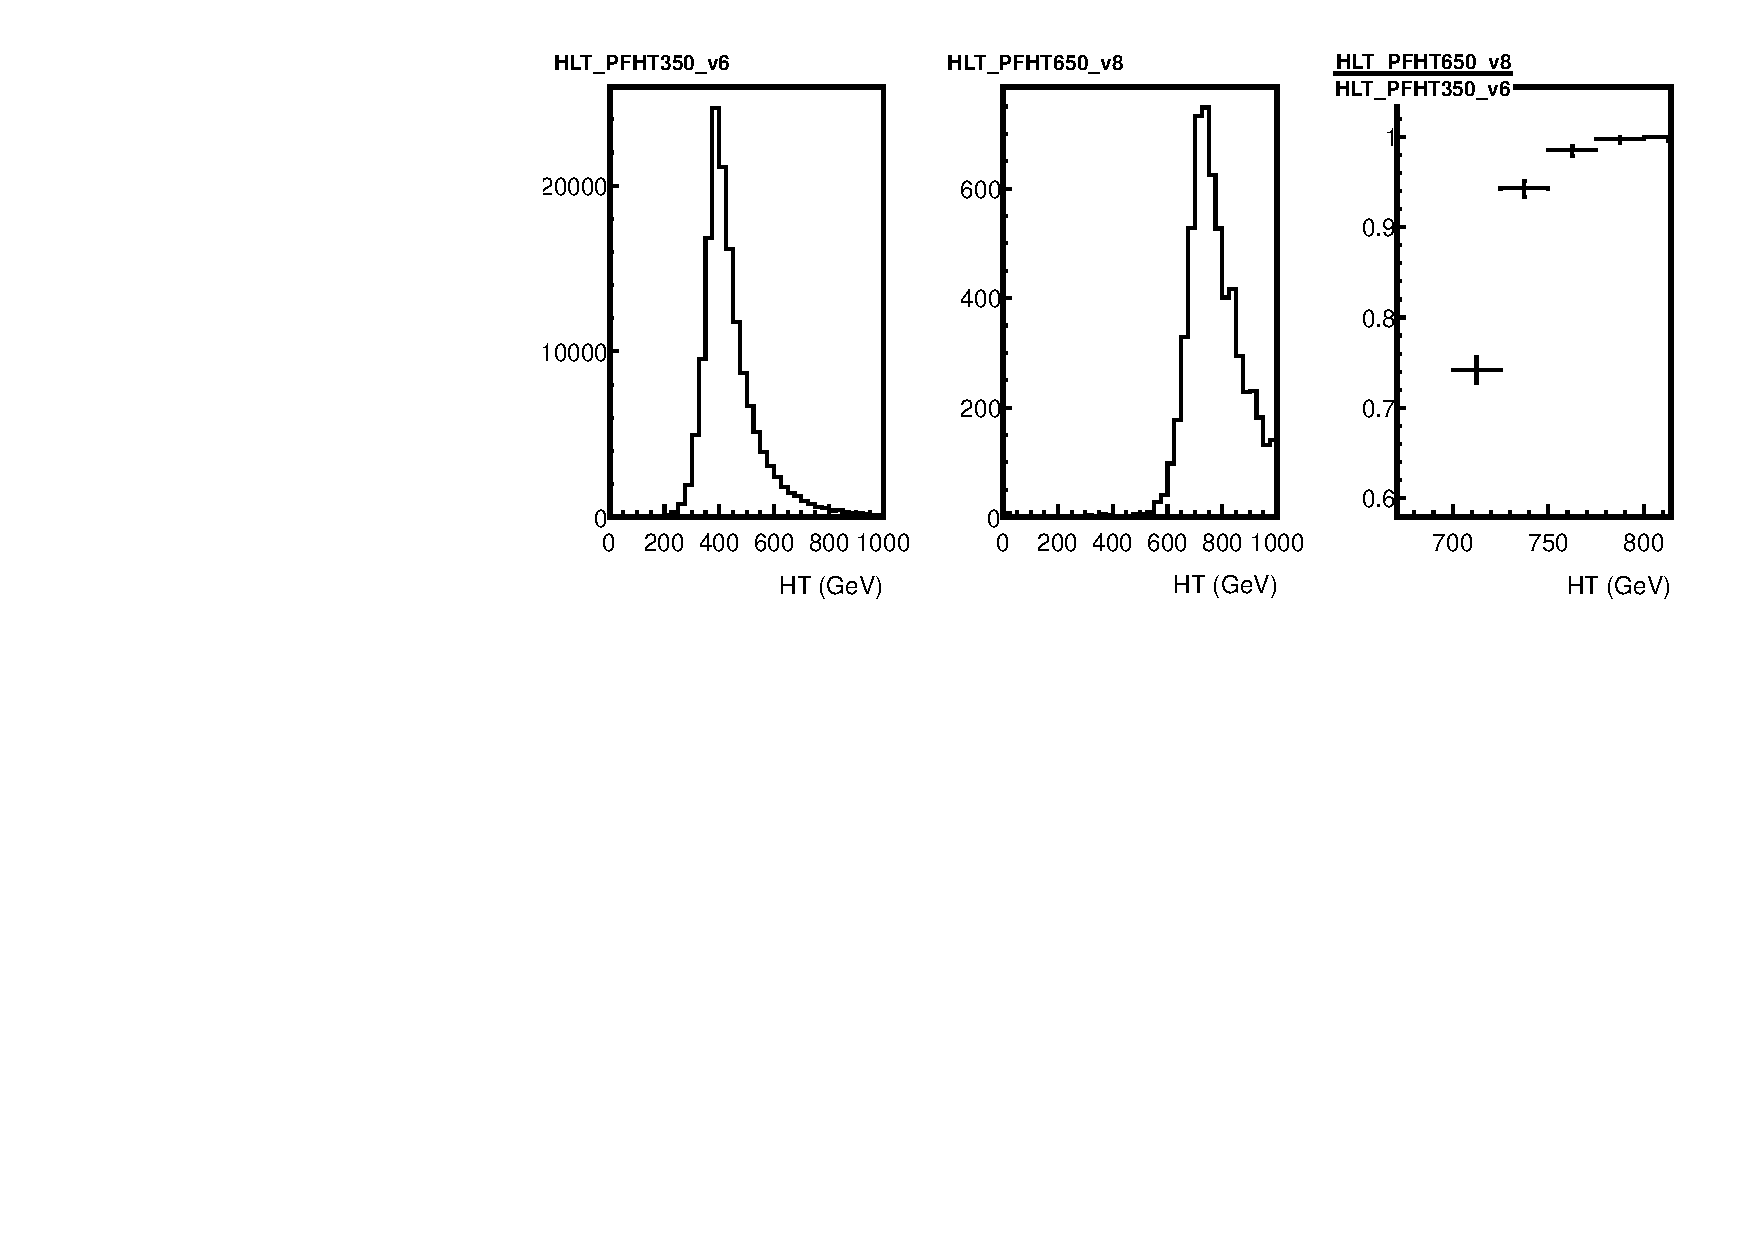
\includegraphics[width=1.0\textwidth]{figs/TriggerDemonstration.pdf}
\caption{The prescaled (left) and  un-prescaled (middle) HT triggers. The right plot shows the ratio of the two previous histograms 
zoomed in the interesting part.}
\label{fig.TriggerPlateau}
\end{figure}
we look at the efficiencies bin-by-bin and distribution of efficiencies (un-prescaled divided by the prescaled, 
figure \ref{fig.TriggerPlateau} (right)) 
with different HT cuts are weighted according to the statistics of the un-prescaled histogram. 
The cut that gives the mean value greater than 95\% is chosen as the offline cut on the trigger parameter. 
An example of this method for different cuts on the HT for HLT\_PFHT650\_vX is shown in figure \ref{fig.TriggerEff}.
\begin{figure}[!htb]
\centering
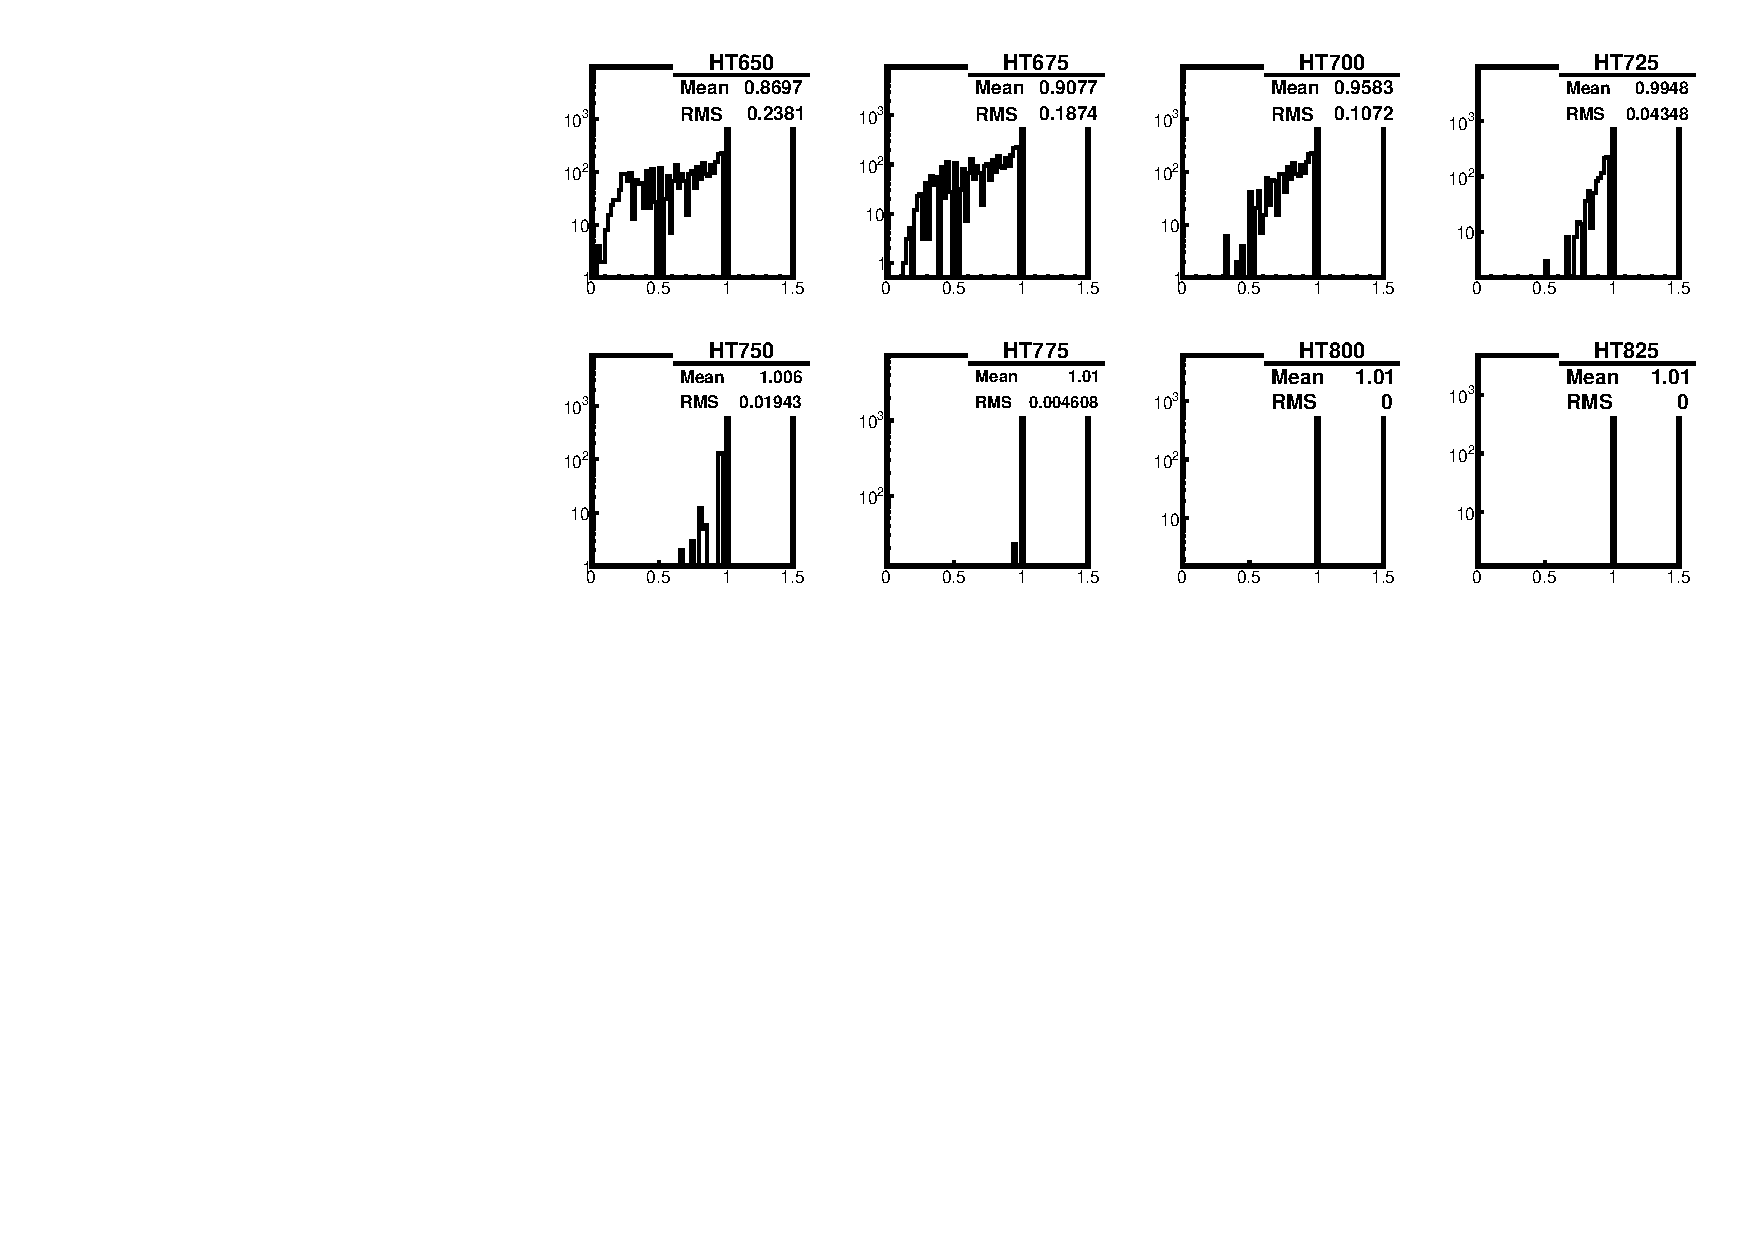
\includegraphics[width=1.0\textwidth]{figs/TriggerDemonstrationEff.pdf}
\caption{The weighted mean of the efficiencies in figure \ref{fig.TriggerPlateau}(right) for different cuts on HT. 
HT $>$ 700 GeV gives 95\% efficiency.}
\label{fig.TriggerEff}
\end{figure}

The result of this method is HT $>$ 700 GeV, but we use 725 GeV conservatively. For the multijet triggers, same method is used and 
depending on the number of jets different cuts on the  $P_T$ of the jets are found. The result is summarized here:
\begin{itemize}
\item HLT\_SixJet45\_vX, 6 jets with \pT $>$ 65 GeV/$c$ or 7 jets with \pT $>$ 55 GeV/$c$
\item HLT\_QuadJet80\_vX, 4 jets with \pT $>$ 100 GeV/$c$ or 5 jets with \pT $>$ 85 GeV/$c$
\end{itemize}
As another possibility, one can think of decreasing the number of jets and increasing the \pT threshold, but it does not reach the
plateau and is excluded from the list.

{\bf FIX ME more material and example can be added if needed!}


\subsection{Trigger Selection}
\label{sect:triggerselection}
To investigate the efficiency of different trigger sets the SMST2tt sample is used. The selection cuts described in section \ref{subsect:mt2bcuts} are applied on top of the trigger selection. The ratio of the signal events passing all the cuts is shown for two different sets of triggers as a function of $\tilde{t}$ mass and $\tilde{\chi^0_1}$ mass in figure \ref{fig:trg_eff}. Although the signal efficiency is $\sim 4$ times larger when the $HT$ trigger is used, MC studies show that the number of remaining backgrounds are so larger that the multi-jet trigger is more powerful to exclude. The estimated exclusion power of both triggers are compared in figure \ref{fig:trgs_exclusion_powers}.

\begin{figure}[htbp] 
\centering
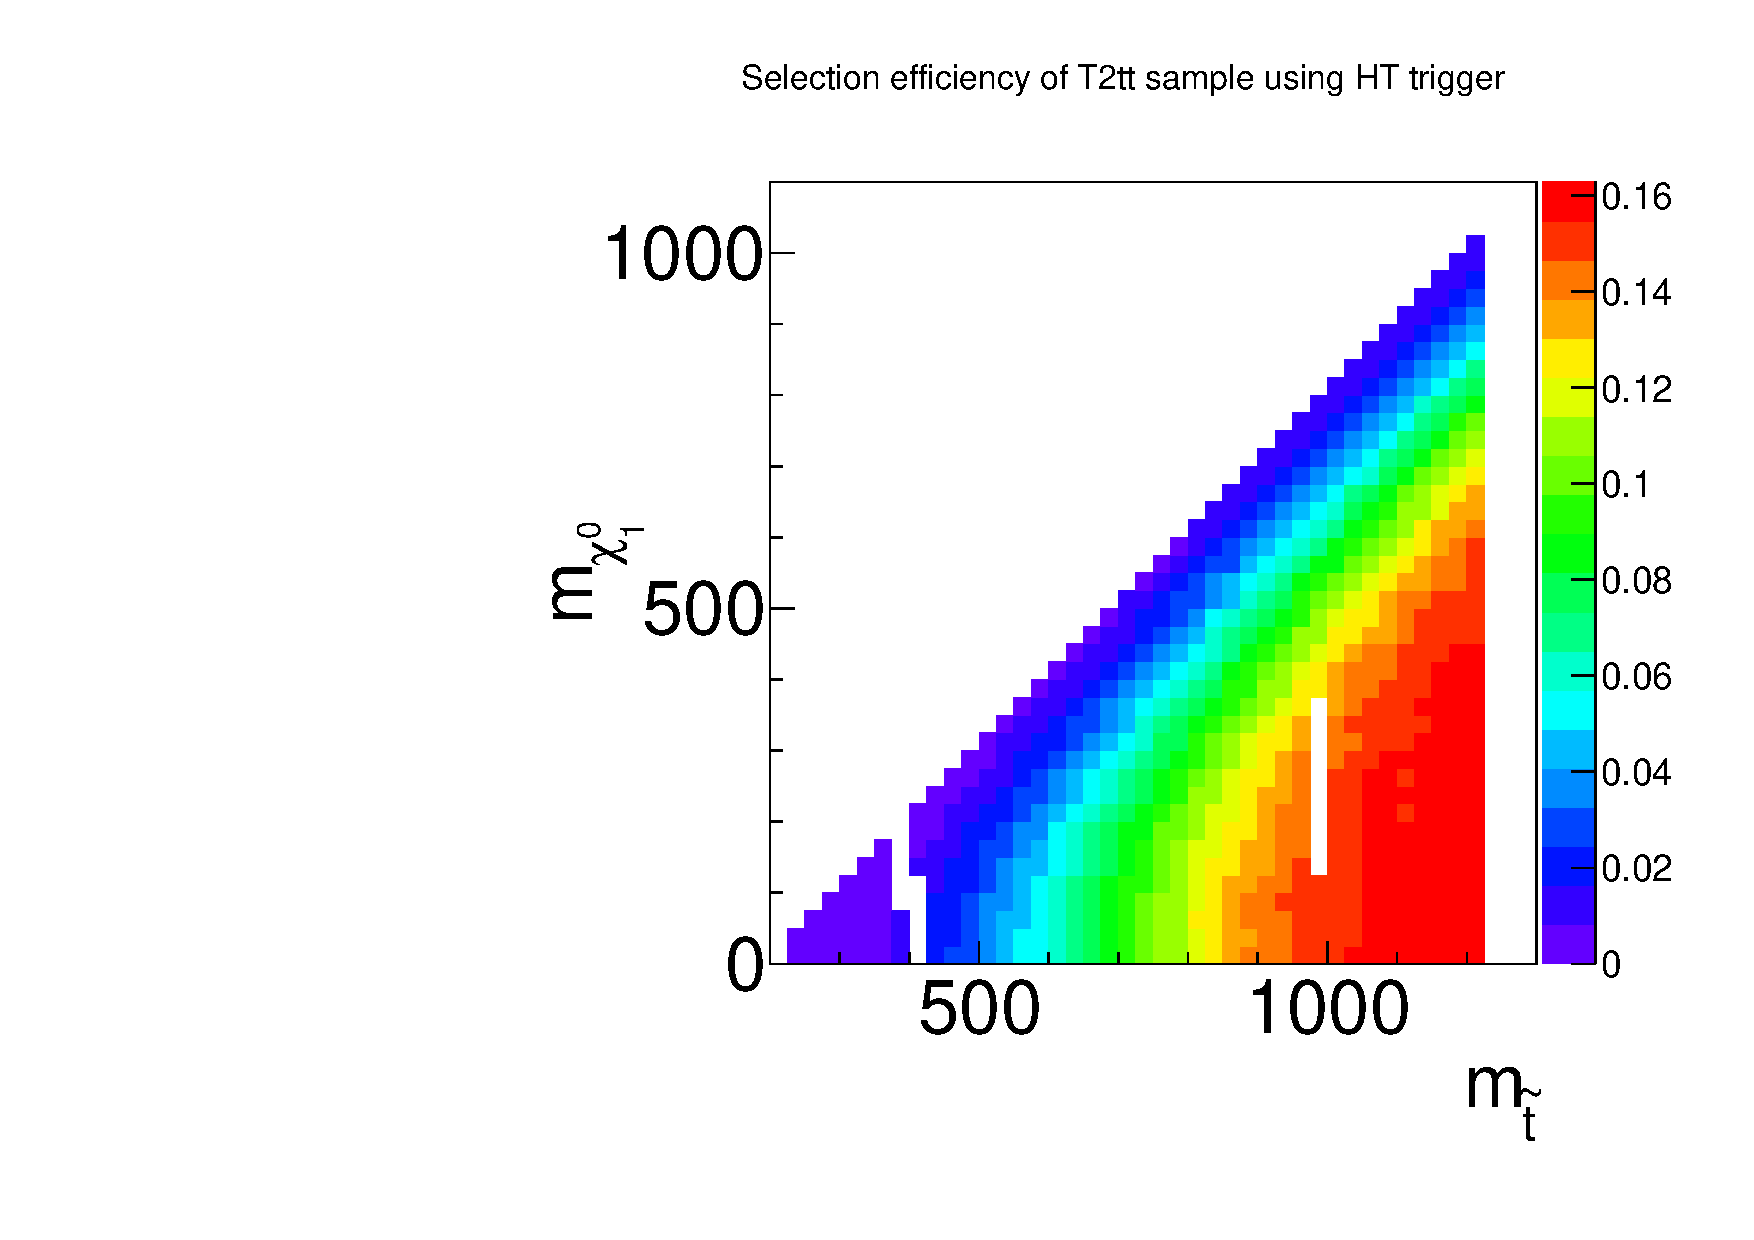
\includegraphics[angle=0,scale=0.39]{figs/HT_eff.pdf}
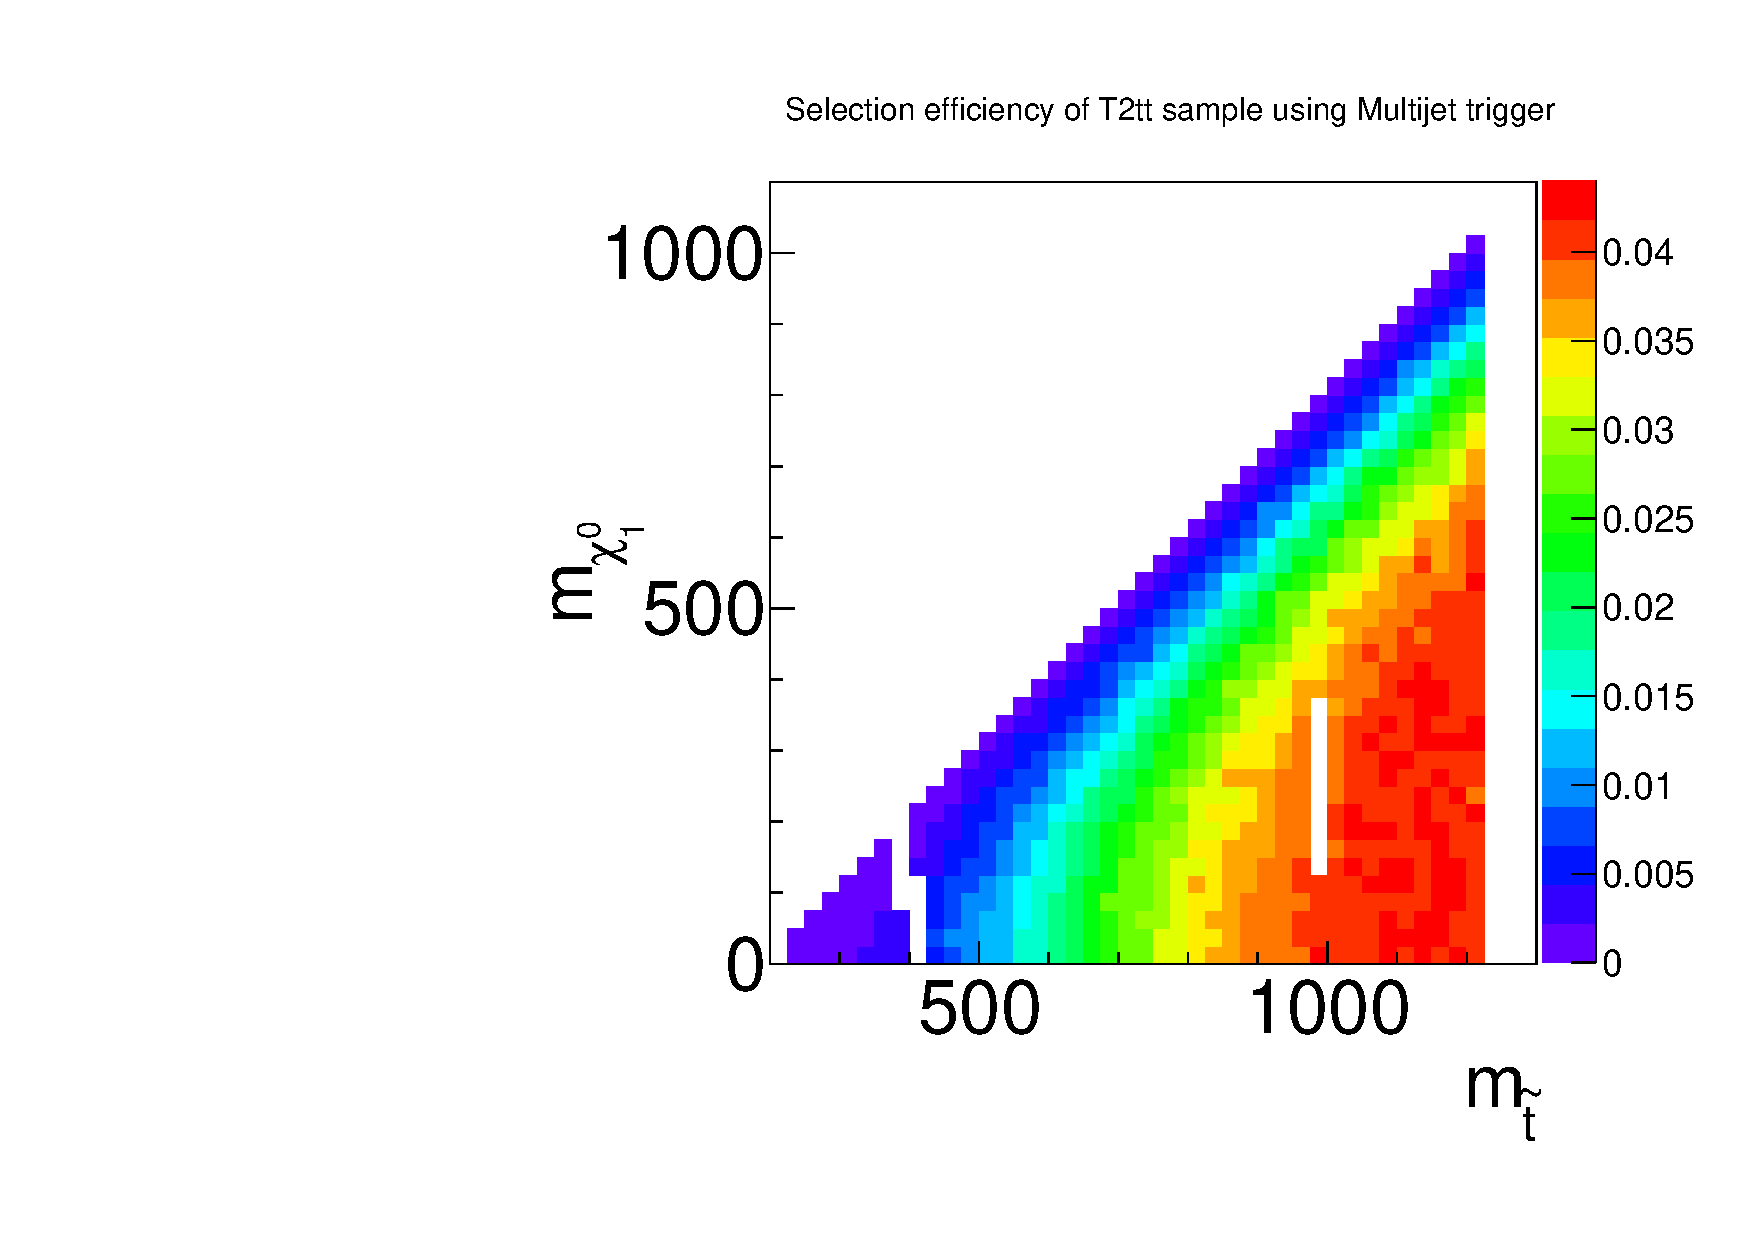
\includegraphics[angle=0,scale=0.39]{figs/multijet_eff.pdf} \\
\caption{The efficiency of different trigger sets (Left : HT trigger, Right : Multijet trigger) for the SMST2tt sample. The results are shown as a function of the $\tilde{t}$ mass and $\tilde{\chi^0_1}$ mass.}
\label{fig:trg_eff}
\end{figure}

\begin{figure}[htbp] 
\centering
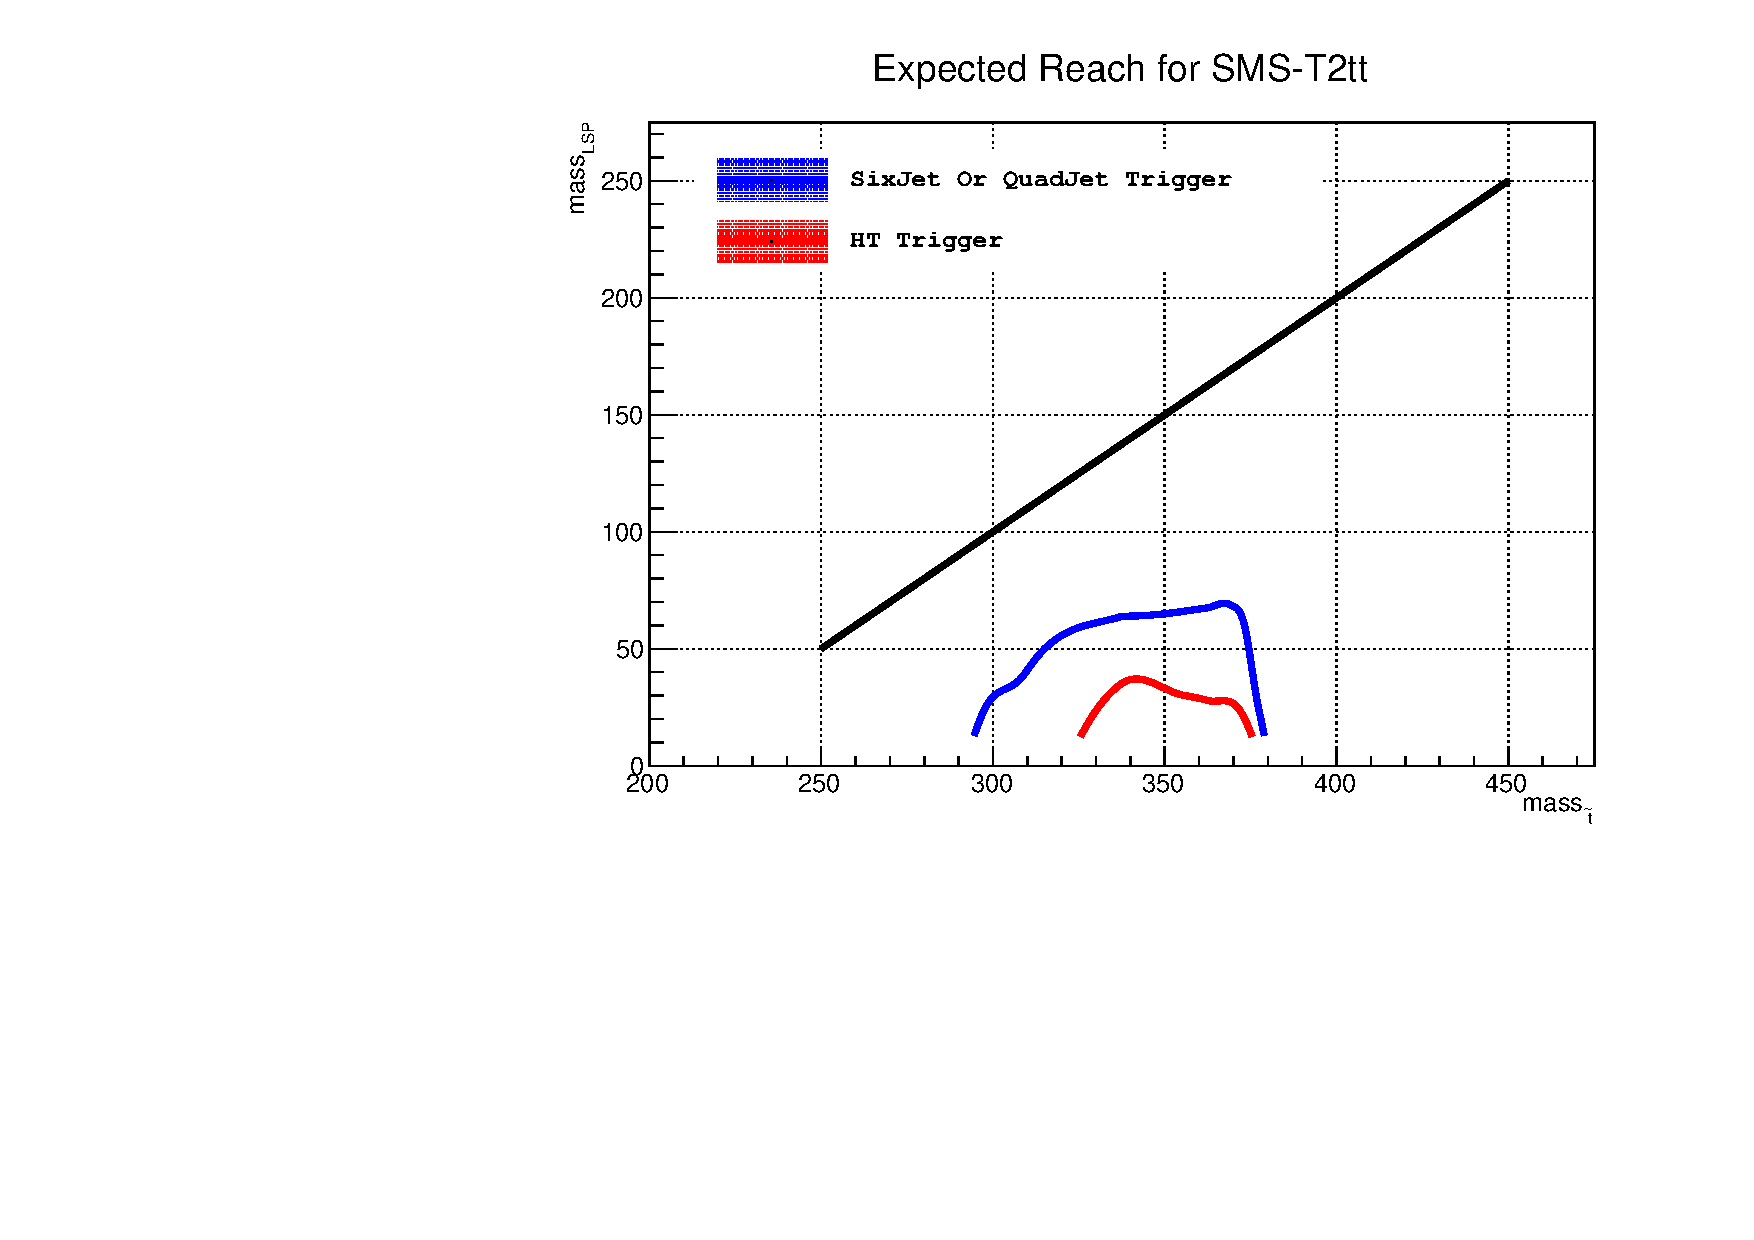
\includegraphics[angle=0,scale=0.5]{figs/SMST2tt_20121114.pdf}
\caption{The estimated exclusion power for two different sets of triggers. The multijet trigger is used in this analysis.}
\label{fig:trgs_exclusion_powers}
\end{figure}

\section{Event Selection}
\subsection{Search Strategy}
\label{sect:cuts}
In this analysis, two leptons are created with two missing particles, so \mttwo can be a good discriminator to separate signal 
from the SM backgrounds that leptons are produced from W or Z boson. When the mass difference between the chargino and neutralino 
is sufficiently large, \mttwo can exceed 80 GeV which is the maximum of the \mt of a lepton which comes from the decay of a W boson.
When the mass difference is not sufficiently large, \mttwo of the signal events is below 80 GeV and the signal is buried under the W+jets
backgrounds. In such conditions, $\Sigma\,\mt$ which is defined as $\mt_{,\ell1} + \mt_{,\ell2}$ can be useful to distinguish between the signal and 
SM backgrounds.
To optimize the cuts, two signal points are selected, one with a high mass difference ($m_{\chipm}$ = 380\,\GeV and $m_{\chiz}$ = 1\,\GeV) and
another one with a low mass difference ($m_{\chipm}$ = 180 GeV and $m_{\chiz}$ = 60 GeV). An optimized cut should minimize the signal strength, 
which is the ratio of the measured upper limit on the cross section and the theoretical signal cross section. The details of the statistical 
method can be found in section \ref{sect:stat}.


\section{Search Strategy}
\label{sect:search}
The \mttwo distribution \ref{fig:MT2}
\begin{figure}[!htb]
\centering
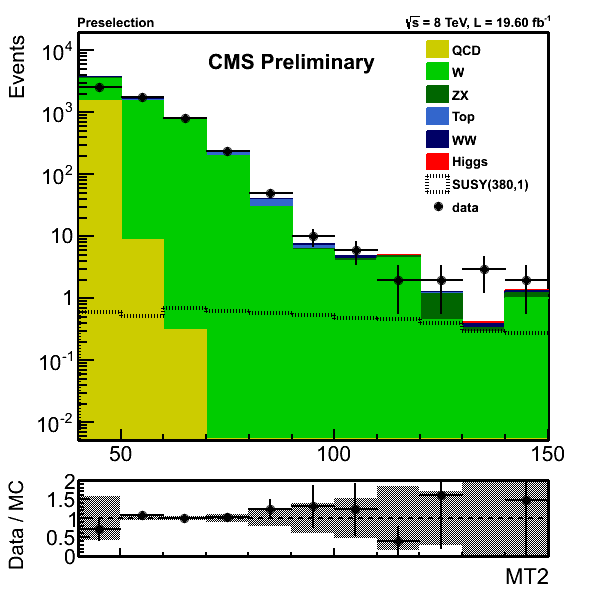
\includegraphics[width=0.49\textwidth]{figs/MT2.png}
\caption{\mttwo distribution after applying the full selection cuts.}
\label{fig:MT2}
\end{figure}
is used as a variable to search for SUSY.
To increase the power of the analysis, a multibinning approach is used.
We select 4 bins in \mttwo with the following edges 125, 150, 200, 250 and infinity.
Every \mttwo bin is devided to two bins with number of the reconstructed top quarks equal to 0 or greater than 0.
There will be 8 bins in the analysis. In this round of analysis, we try to emphasize the complementary role of this anaysis
for the common cut and count hadronic search for the direct stop production. Since this analysis, does not use the MET explicitly, 
it is more sensetive to the small mass differences between stop and LSP.
\section{Backgrounds}
\label{sect:bkg}
In this section, data driven methods are proposed and applied to estimate the contribution of the main background processes. 
Most of the methods are similar to what were used in the \mttwo analysis \cite{MT2_2011} with some minor changes which are explained
here.


 
\subsection[QCD Estimation]{Data-driven background estimation of QCD}\label{subsect:qcd}

Due to inadequate statistics of QCD Monte-Carlo samples and complicated nature of this background, 
we use a data driven method to estimate its rate in the tails of the $\mttwo$ distribution, while the simulation shows that it is 
negligible.

We follow the method, fully discussed and applied by the $\mttwo$ and $M_{T2b}$ groups \cite{MT2_2011},
 but the parameters are finely tuned to the conditions of our analysis.
The method indeed relies on different distributions of QCD and SUSY-like events 
in the plane of $\mttwo$ and $\mindphifour$, 
the azimuth-difference between the $\met$ vector and the closest selected jet.

%%%%%%%%%%
\begin{linenomath}
\begin{figure}[h]
\centering
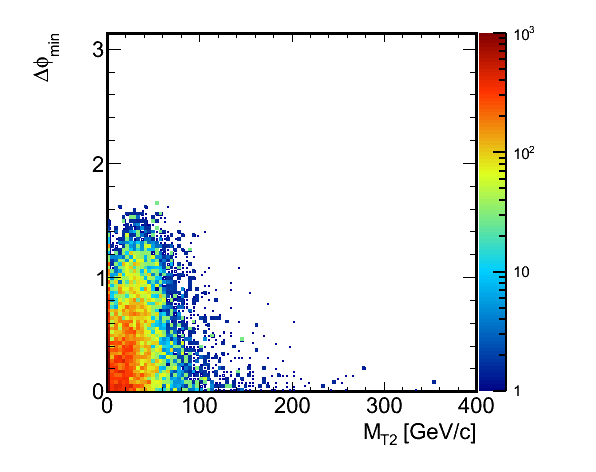
\includegraphics[width=0.49\textwidth,keepaspectratio=true]{QCDFig/qcd_distribution.png}
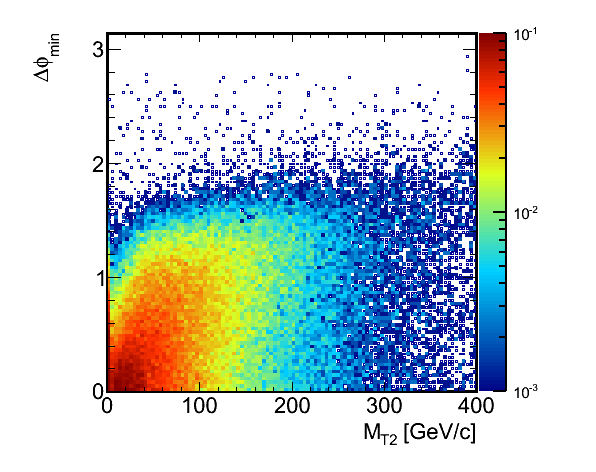
\includegraphics[width=0.49\textwidth,keepaspectratio=true]{QCDFig/sms_distribution.png}
\caption[DPhi vs. MT2 Distribution]{Distribution of $\mindphifour$ versus $\mttwo$ for (left) QCD and 
(right) SUSY-like (SMS) simulated events. QCD events are populated in the low $\mindphifour$ and $\mttwo$ region, while
SUSY events spread over the plane.}
\label{fig:distributions}
\end{figure}
\end{linenomath}
%%%%%%%%%%

Figure \ref{fig:distributions} shows such distributions for QCD (left) and SMS samples (right).
Unlike the broad spread of SMS events in this plane, QCD events are densely populated 
in the low $\mindphifour$ and $\mttwo$ region.
Due to the strong correlation between the two variables of $\mindphifour$ and $\mttwo$, 
the usual ABCD method is inefficient, whereas a factorization method \cite{MT2_2011} is still applicable.
The method works based on the ratio of $r(\mttwo) = N (\mindphifour \geq 0.3)/N (\mindphifour \leq 0.2)$ 
as a function of $\mttwo$ for QCD events. Figure [\ref{fig:qcd_ratio}] shows the ratio $r(\mttwo)$ in the QCD simulation. 
It indicates an exponentially descending behavior
%  of the ratio $r(\mttwo)$ for the QCD simulation on 
in the region of $\mttwo > 50$ GeV (the lower bins of $\mttwo$ could be biased by the minimal cut on $\met$). 
Hence, we characterize such specification of the QCD events by the model 
of 
%%%%%%%%%%  
\begin{align}\label{eq:rmt2}
 r(\mttwo) = \frac{N(\mindphifour \geq 0.3)}{N(\mindphifour \leq 0.2)} = e^{a-b.\mttwo}+c
\end{align}
%%%%%%%%%%

% where the parameters of $b$ and $a$ indicate slope-intercept form of the straight line
where a and b parameters indicate respectively the slope and the intercept of the straight line
 in the logarithmic scale. 
Function \ref{eq:rmt2} tends towards 
% the constant value of c at the large value of $\mttwo$.
constant value, c, at large values of $\mttwo$.
The red curve in Figure \ref{fig:qcd_ratio} shows the fit of a model \ref{eq:rmt2} to the QCD simulation and 
Table \ref{tab:qcd_fit} presents the value of parameters as a result of the fit in the range of $\mttwo > 50$ GeV (the first column). 

%%%%%%%%%%
\begin{linenomath}
\begin{table}[h]
\begin{center}
\small
\begin{tabular}{l|cc}\hline\hline
Parameter & $\mttwo > 50$ GeV & $50 > \mttwo > 90$ GeV \\ \hline
a	&	$1.757\pm0.090$	&	$1.847\pm0.097$	\\
b (GeV$^{-1}$)	& $0.0201\pm0.0011$	&	$0.0213\pm0.0012$	\\
c	&	$0.0020\pm0.0028$	&	-	\\ \hline\hline
\end{tabular}
\caption[Fit results for QCD]{The result of the two different parametrizations for ratio $\rm{r(\mttwo)}$ in QCD simulated events.}  
\label{tab:qcd_fit}
\end{center}
\end{table}
\end{linenomath}
%%%%%%%%%%

In real data, to have a pure QCD sample with the minimal contamination from non-QCD backgrounds, we have to 
concentrate on the region of low $\mttwo$ ($50 < \mttwo < 90$ GeV). 
The fit of ratio $r(\mttwo)$ on this short range of $\mttwo$ can be reasonably described as a straight line in the logarithmic scale.
Thus, it is not able to give parameter c. 
The green curve in Figure \ref{fig:qcd_ratio} shows the linear fit and 
the second column of Table \ref{tab:qcd_fit} presents the relevant parameters, a and b.
As taken from Figure \ref{fig:qcd_ratio}, both fits (green and red) are in 
a very good agreement at low $\mttwo$, while the second fit (the green straight line), 
called optimistic parameterization, gives the lower values for ratio $r(\mttwo)$ 
at high $\mttwo$. 
Hence, a realistic model needs also the parameter c to parameterize 
the ratio $r(\mttwo)$ in the entire range of $\mttwo$. 
% To solve the arisen problem 
we conservatively 
% chose to 
take the parameter c from the straight line at $\mttwo = 250$ GeV. 
The blue curve of Figure \ref{fig:qcd_ratio} represents such a fit, 
namely pessimistic parameterization. 

%%%%%%%%%%
\begin{linenomath}
\begin{figure}[h]
\centering
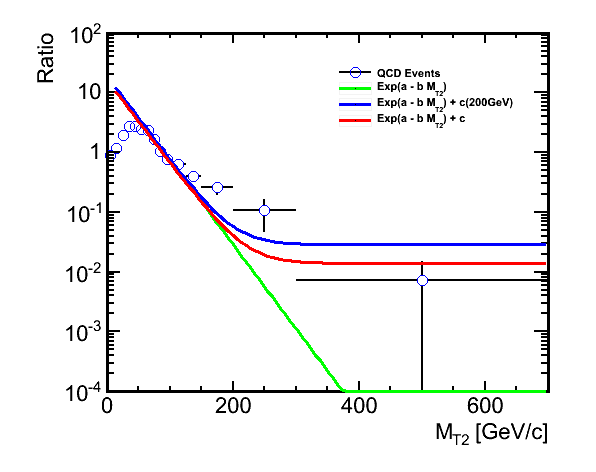
\includegraphics[width=0.7\textwidth,keepaspectratio=true]{QCDFig/qcd_ratio.png}
\caption{Three different fits of ratio $r(\mttwo)$  in QCD simulated events. 
The red curve is an exponential function plus a constant. It uses
the entire range of $\mttwo > 50$ GeV for parametrization (fully-MC) of ratio $r(\mttwo)$. 
The green curve is just an exponential function and uses the range of $50 < \mttwo < 90$ GeV 
for parameterization (optimistic). 
The blue curve is also an exponential function plus a constant, 
however it uses the range of $50 < \mttwo < 90$ GeV for parameterization (pessimistic).}
\label{fig:qcd_ratio}
\end{figure}
\end{linenomath}
%%%%%%%%%%

Figure \ref{fig:data_ratio} depicts both parameterizations 
(optimistic and pessimistic by green and blue curves respectively) 
as a consequence of employing the method in the cleaned data.
The non-QCD contaminations, taken from the Monte-Carlo simulation, are subtracted from 
data before calculating the parameters.
Table \ref{tab:data_fit} presents the parameters a and b extracted from the fit. 
These data-driven parameters eventually fulfill the functional form of ratio $r(M_{MT2})$.

%%%%%%%%%%
\begin{linenomath}
\begin{figure}[h]
\centering
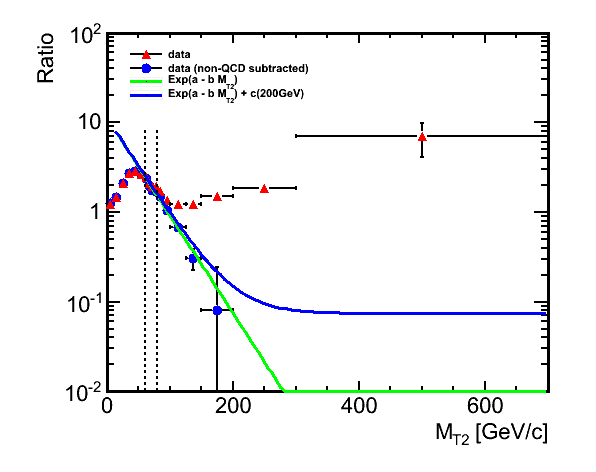
\includegraphics[width=0.49\textwidth,keepaspectratio=true]{QCDFig/data_ratio.png}
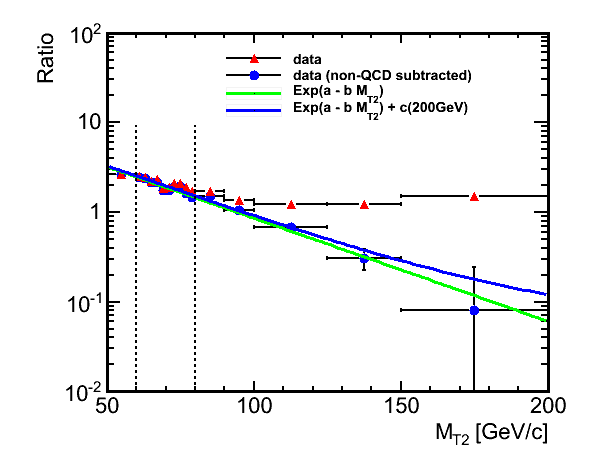
\includegraphics[width=0.49\textwidth,keepaspectratio=true]{QCDFig/data_ratio_zoom.png}
\caption{Fits of ratio $r(\mttwo)$ in the non-QCD subtracted data. 
The green and blue curves are related to optimistic
and pessimistic parameterization respectively. The right plot is a focus on the desired range of $\mttwo$ for the parametrizations.} 
\label{fig:data_ratio}
\end{figure}
\end{linenomath}
%%%%%%%%%%


%%%%%%%%%%
\begin{linenomath}
\begin{table}[h]
\begin{center}
\small
\begin{tabular}{l|c}\hline\hline
Parameter & $50 > \mttwo > 90$ GeV \\ \hline
a	&	$2.16\pm0.13$	\\
b (GeV$^{-1}$)	&	$0.0209\pm0.0020$	\\ \hline\hline
\end{tabular}
\caption[Fit results for data]{The parametrization results for ratio $\rm{r(\mttwo)}$ 
in real data (non-QCD events are subtracted, using simulation).}
\label{tab:data_fit}
\end{center}
\end{table}
\end{linenomath}
%%%%%%%%%%

In the last step of procedure, we apply the ratio $r(\mttwo)$ 
to the observed cleaned data in the QCD control region (high $\mttwo$, 
low $\mindphifour$) to estimate the number of QCD events in the signal region 
(high $\mttwo$, high $\mindphifour$). Figure \ref{fig:exp_distribution} shows 
the $\mttwo$ distribution of QCD truth observed events and 
the expected distribution from data (non-QCD subtracted). 
Furthermore, Table \ref{tab:exp_distribution} compares
the estimated with observed QCD events for several bins of $\mttwo$.
%%%%%%
In addition to the statistical uncertainties, the predicted numbers incorporate the systematic ones, coming from
the fit range. Indeed, the standard deviation of a $10\%$ fluctuation at the boundaries of the fit range, $(50 < \mttwo < 90)$ GeV, 
induces the systematic uncertainties reported in Table \ref{tab:exp_distribution}. 
%%%%%%
Considering the uncertainties, the method prediction is in good agreement with the QCD truth. 
 
%%%%%%%%%%
\begin{linenomath}
\begin{figure}
\centering
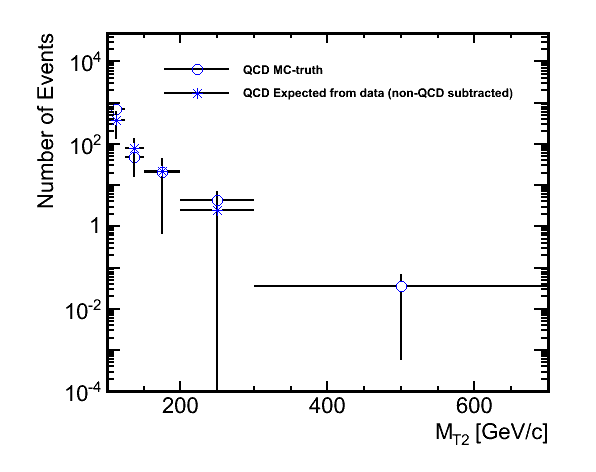
\includegraphics[width=0.7\textwidth,keepaspectratio=true]{QCDFig/exp_distribution.png}
\caption{QCD MC-truth and data-driven prediction for the distribution of $\mttwo$.}
\label{fig:exp_distribution}
\end{figure}
\end{linenomath}
%%%%%%%%%%

%%%%%%%%%%
\begin{linenomath}
\begin{table}[h]
\begin{center}
\small
\begin{tabular}{l|cc}\hline\hline
$\mttwo$ bins & MC-truth & Data-prediction \\ \hline
$[125, 150)$	&	$36.4\pm28.0$		& $23.3\pm14.8\pm4.5$ \\
$[150, 200)$	&	$4.6\pm2.1$			& $6.8\pm5.4\pm2.0$ \\
$[200, 300)$	&	$0.20\pm0.14$		& $0.33\pm0.63\pm0.16$ \\
$[300, inf)$	&	$0.0043\pm0.0042$	& $0.03\pm0.11\pm0.02$ \\ \hline\hline
\end{tabular}
\caption{QCD MC-truth and data-driven prediction for the several bins of $\mttwo$.}
\label{tab:exp_distribution}
\end{center}
\end{table}
\end{linenomath}
%%%%%%%%%%







\subsection{Data-Driven Estimation of Lost Lepton from W+jets and Top}
\label{sect:intro}
After applying the selection cuts, described in detail in Section~\ref{sect:cuts}, the background 
events are dominated by $t\bar t$ events. Among all decay channels of top pair system, 
it is mainly the semi-leptonic decay which contributes to the background. 
This can be understood because genuine neutrino is produced in the semi-leptonic decay of 
top pair system, $t\bar t\rightarrow W^+bW^-\bar b\rightarrow b\bar bl\nu_ljj$, 
which can pass the $M_{T2}$ cut while the full-hadronic decay products, $t\bar t\rightarrow W^+bW^-\bar b\rightarrow b\bar bjjjj$, do not contain any neutrino.
This section describes a method to estimate the backgrounds from the leptonic decay of $W$ bosons, 
either from prompt production in $W+$jets events or from $W$ bosons produced in single top and 
top pair events, shown as $t(\bar t)$ for simplicity. The lepton is considered to be electron or muon.\\
Although the leptons are vetoed in the main analysis, but there are still some background 
from $W\rightarrow l\nu_l$, referred to as lost lepton background events, 
contributing to the full-hadronic analysis. This is due to the acceptance cuts or 
inefficiencies in the lepton isolation and identification criteria.\\
In order to estimate the backgrounds due to the lost lepton events, all selection cuts are applied except
 lepton veto which is inverted. The distribution of the $p_T$ of the leptons in the events 
with exactly one lepton, being either electron or muon, are shown in 
Figure~\ref{fig:pt}, where it can be seen that the number of MC events are greater than the 
observed number of data events.\\
\begin{figure}[htbp] 
\centering
%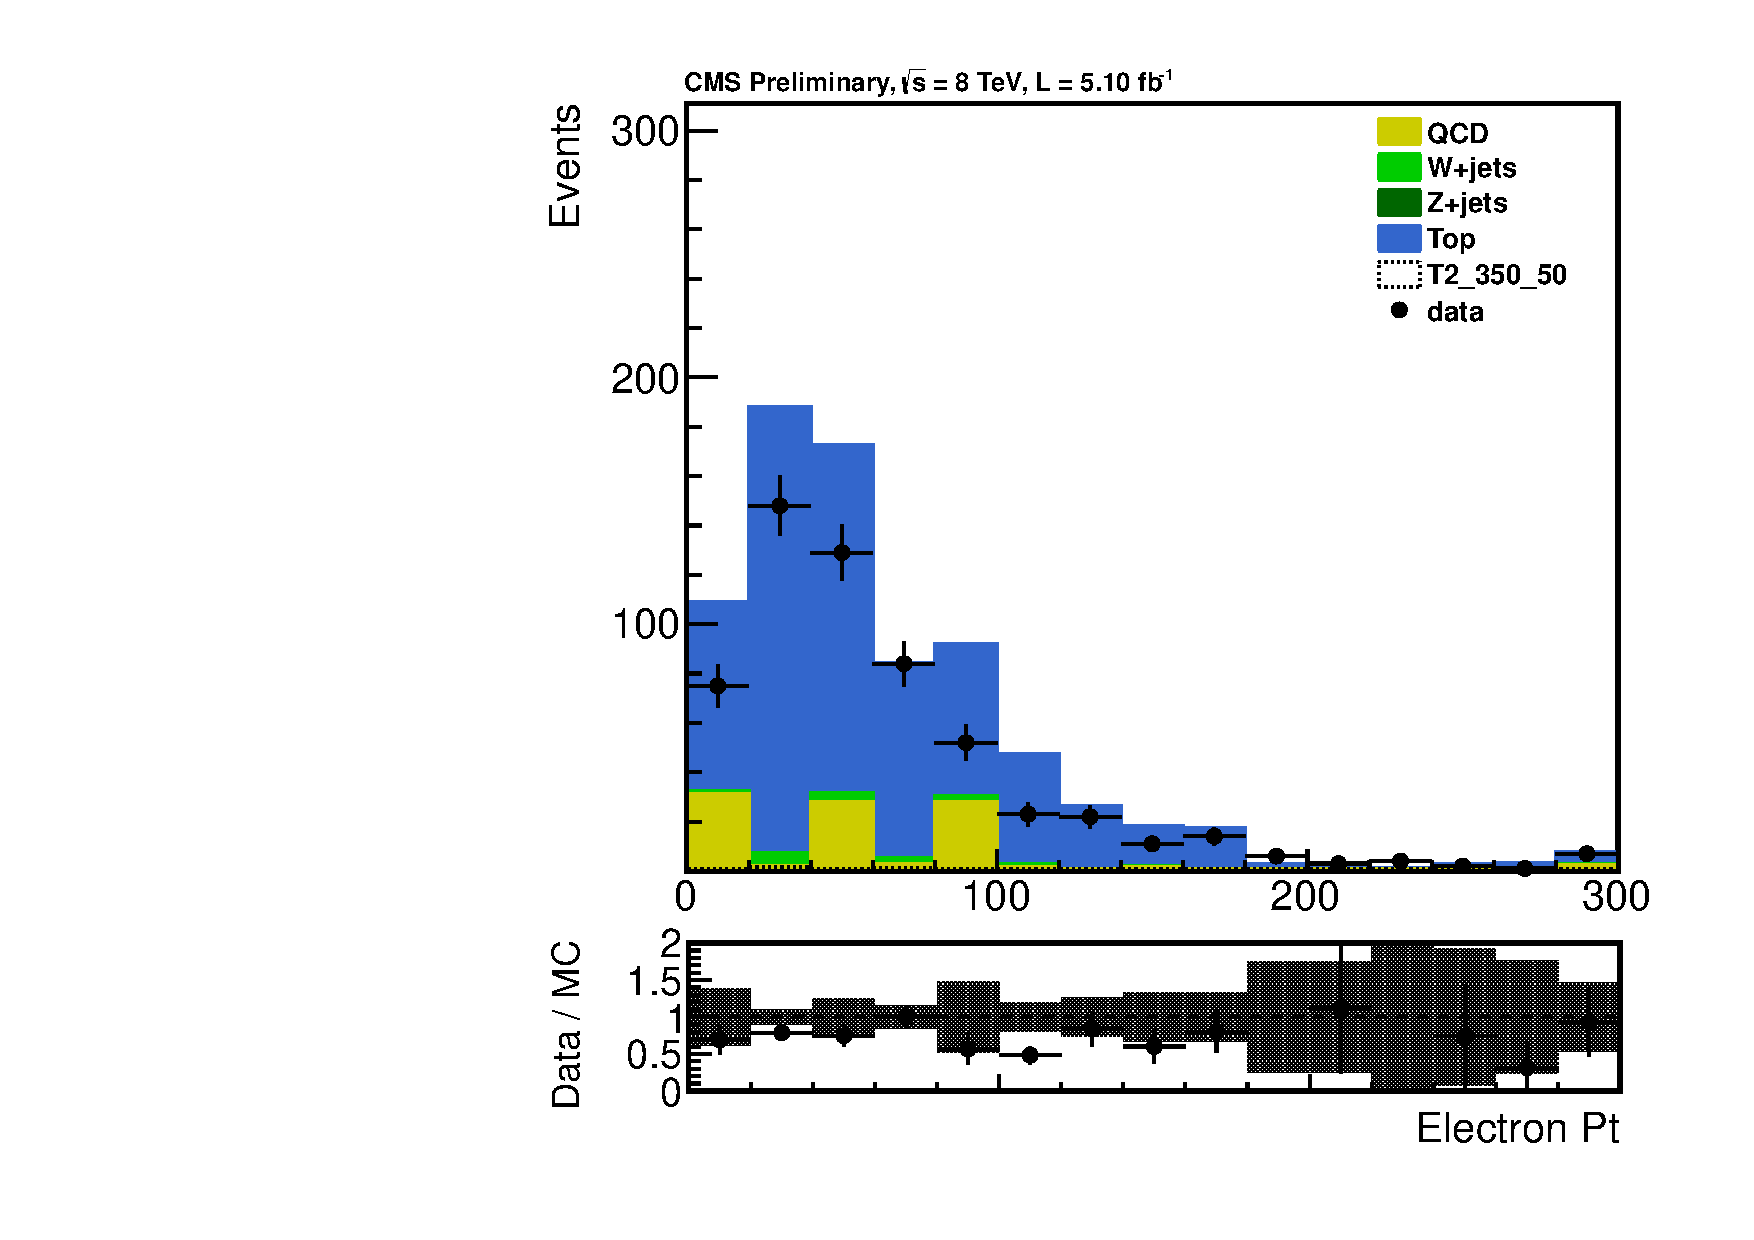
\includegraphics[angle=0,scale=0.39]{myplots/ele_pt.pdf}
%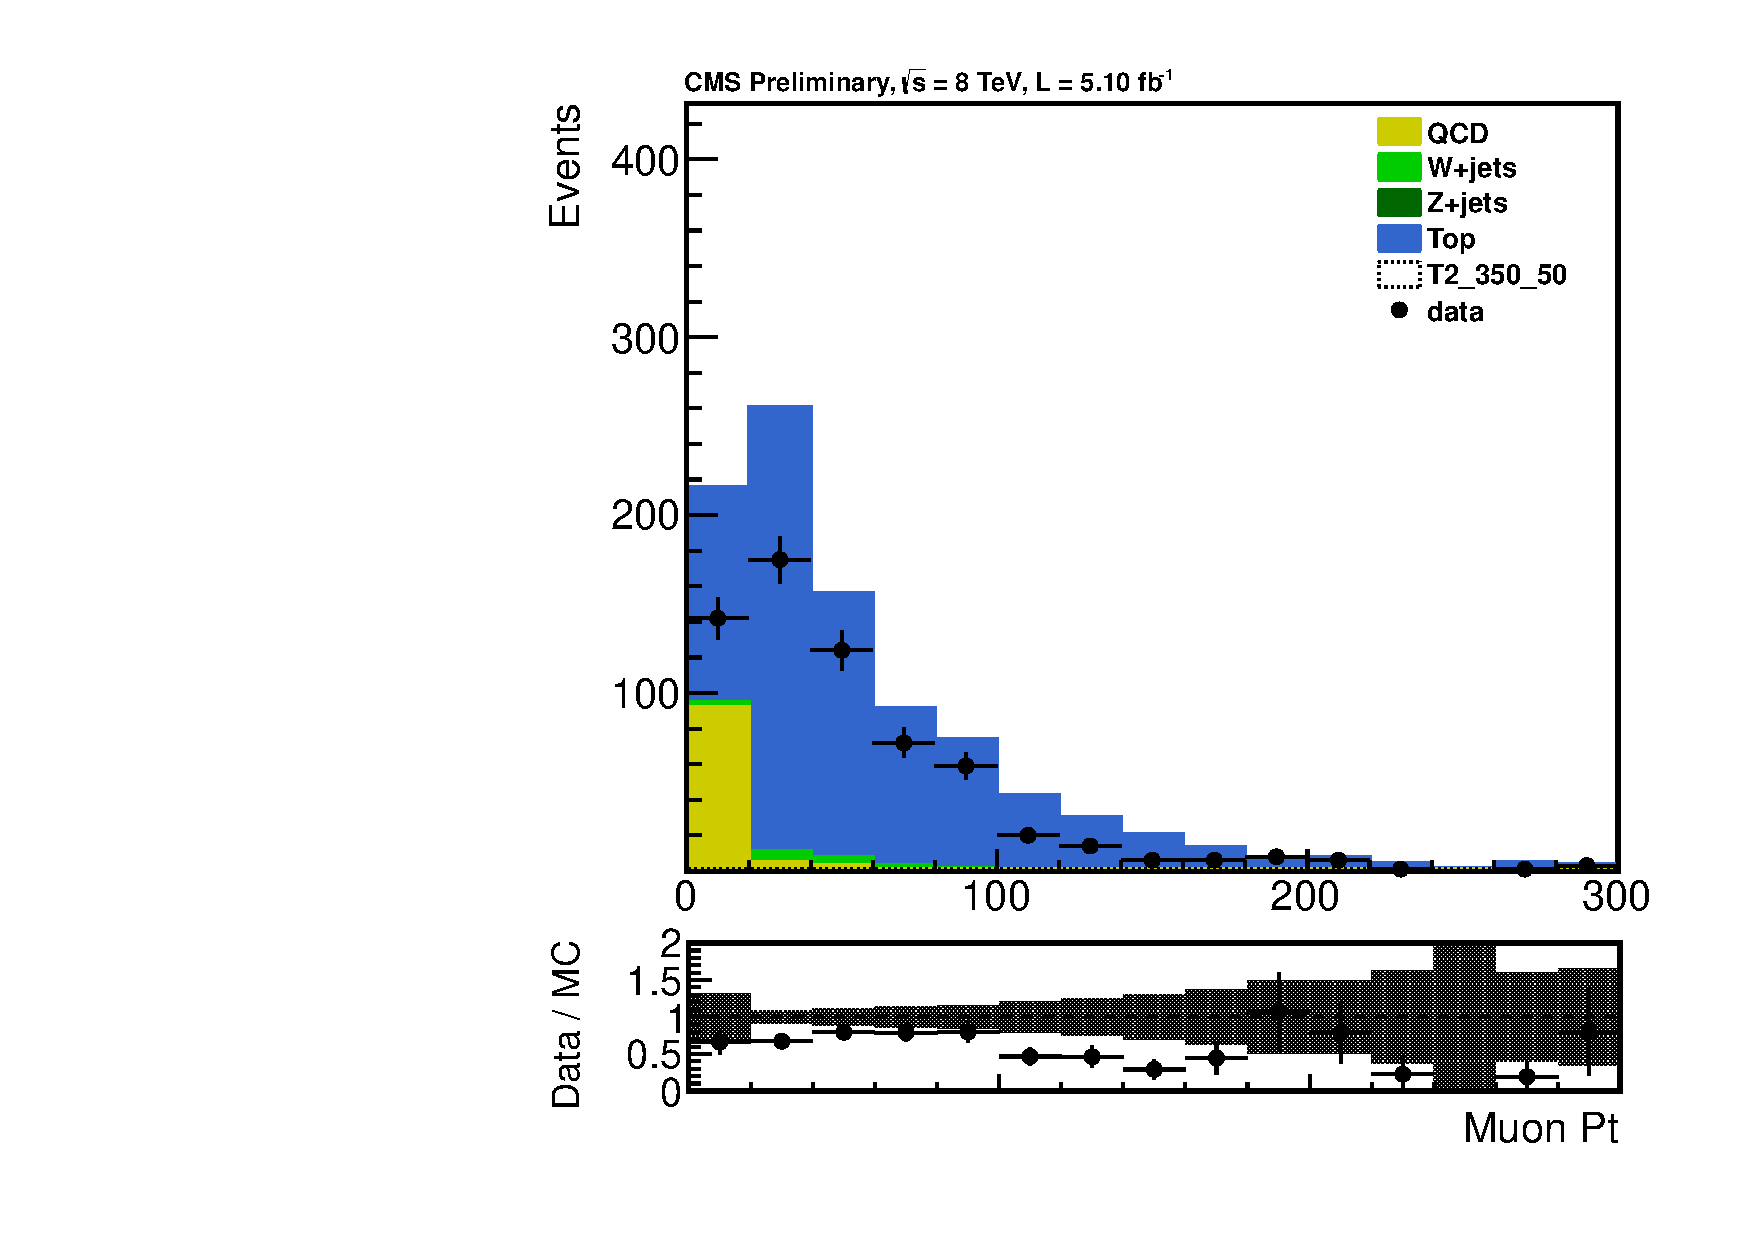
\includegraphics[angle=0,scale=0.39]{myplots/muo_pt.pdf} \\
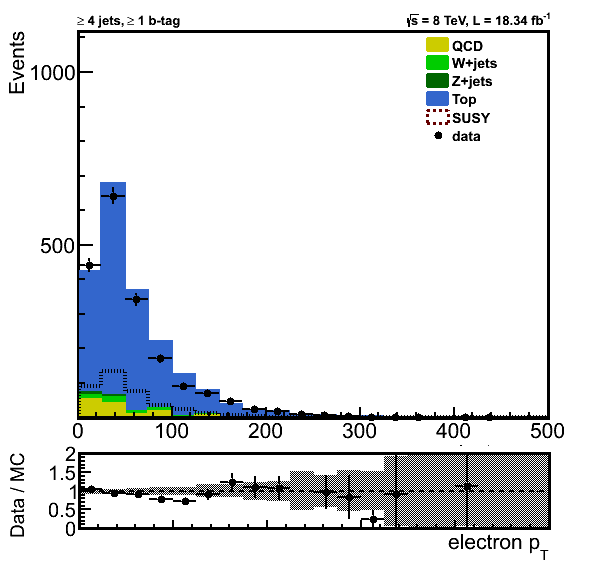
\includegraphics[angle=0,scale=0.35]{llplots_20Invfb/ele_pt.png}
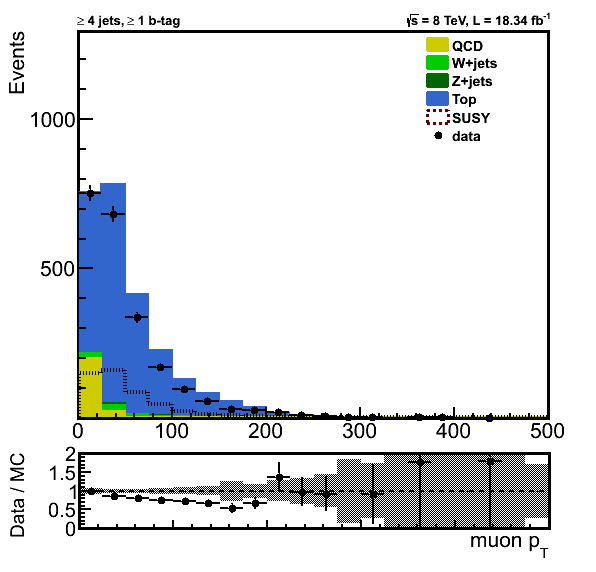
\includegraphics[angle=0,scale=0.35]{llplots_20Invfb/mu_pt.png} \\
\caption{Left: The $p_T$ distribution of the electrons in the events with one electron 
passing all selection cuts but the \mindphifour cut. The reason for this is stated in the text. No $M_{T2}$ cut is applied in 
order to have more statistics. Right: The same plot for muons.}
\label{fig:pt}
\end{figure}

In order to increase the data statistics, the cut on the 
\mindphifour is relaxed. While this cut was introduced in the main analysis to suppress the $QCD$ background events, now that 
the lepton veto is reversed and exactly one lepton is required, the $QCD$ events are still under control. 
Hence relaxing the \mindphifour cut would not be harmful. The only thing which should be taken into account 
is to consider the efficiency of this cut, called as $f$, which is explained in the following.\\
The contribution of the lost lepton background events passing the lepton veto, shown as $N_l^{pass}$, is estimated with the following formula
\begin{eqnarray} 
N_l^{pass}&=&(N_l^{reco}-N_l^{bg})\frac{1}{\varepsilon_l}-(N_l^{reco}-N_l^{bg})\\\nonumber
&=&(N_l^{reco}-N_l^{bg})\frac{1-\varepsilon_l}{\varepsilon_l},\nonumber
\end{eqnarray}
where $N_l^{reco}$ refers to the number of data events with all selection cuts but the inverted 
lepton veto, which requires exactly one lepton. For this set of cuts, the number of background events from processes 
other than $W\rightarrow l\nu_l$ is represented by $N_l^{bg}$ and is taken from MC. The $\varepsilon_l$ contains 
the efficiency for a generated $W\rightarrow l\nu_l$ passing all selection cuts but the inverted lepton veto to have a 
lepton reconstructed. Here, the electron and muon efficiencies are obtained from both $t\bar t$ and $W+jets$ events and a relative contribution is used in the above formula. It should also be noted that, at the generator level, those $t\bar t$ events containing a tau lepton decaying hadronically are vetoed since these kind of events are considered when backgrounds from tau are estimated.\\ 
In order to reduce the signal contamination in the leptonic signal region, a cut on the transverse mass of the 
lepton, $m_T$, is applied which is defined as
$$m_T=\sqrt{2p_T(e,\mu)E_T^{miss}(1-\cos(\Delta\Phi))} < 100\; \rm GeV,$$
where $\Delta\Phi$ is the angle between lepton-$p_T$ and $E_T^{miss}$ in the transverse plane. 
In the $W\rightarrow l\nu_l$ events, the $m_T$ cut represents the transverse mass of 
the $W$ bosons which decreases above $80$ GeV. Hence the leptonic signal events are not 
affected by this cut, while the contamination from SUSY events are strongly suppressed. The 
distribution of the $m_T$ of either electrons or muons in the events with exactly one electron and one muon respectively, are shown in
Figure~\ref{fig:mt}. In this analysis, 
it is found that, e.g. for electron $m_T$ distribution, the $S/B$ decreases from $1.03\%$ to $0.60\%$ when $m_T<100$ GeV cut is introduced. In 
the rest of this section, in addition to all selection cuts, the leptons are required to pass $m_T<100$ GeV cut.\\ 
\begin{figure}[htbp] 
\centering
%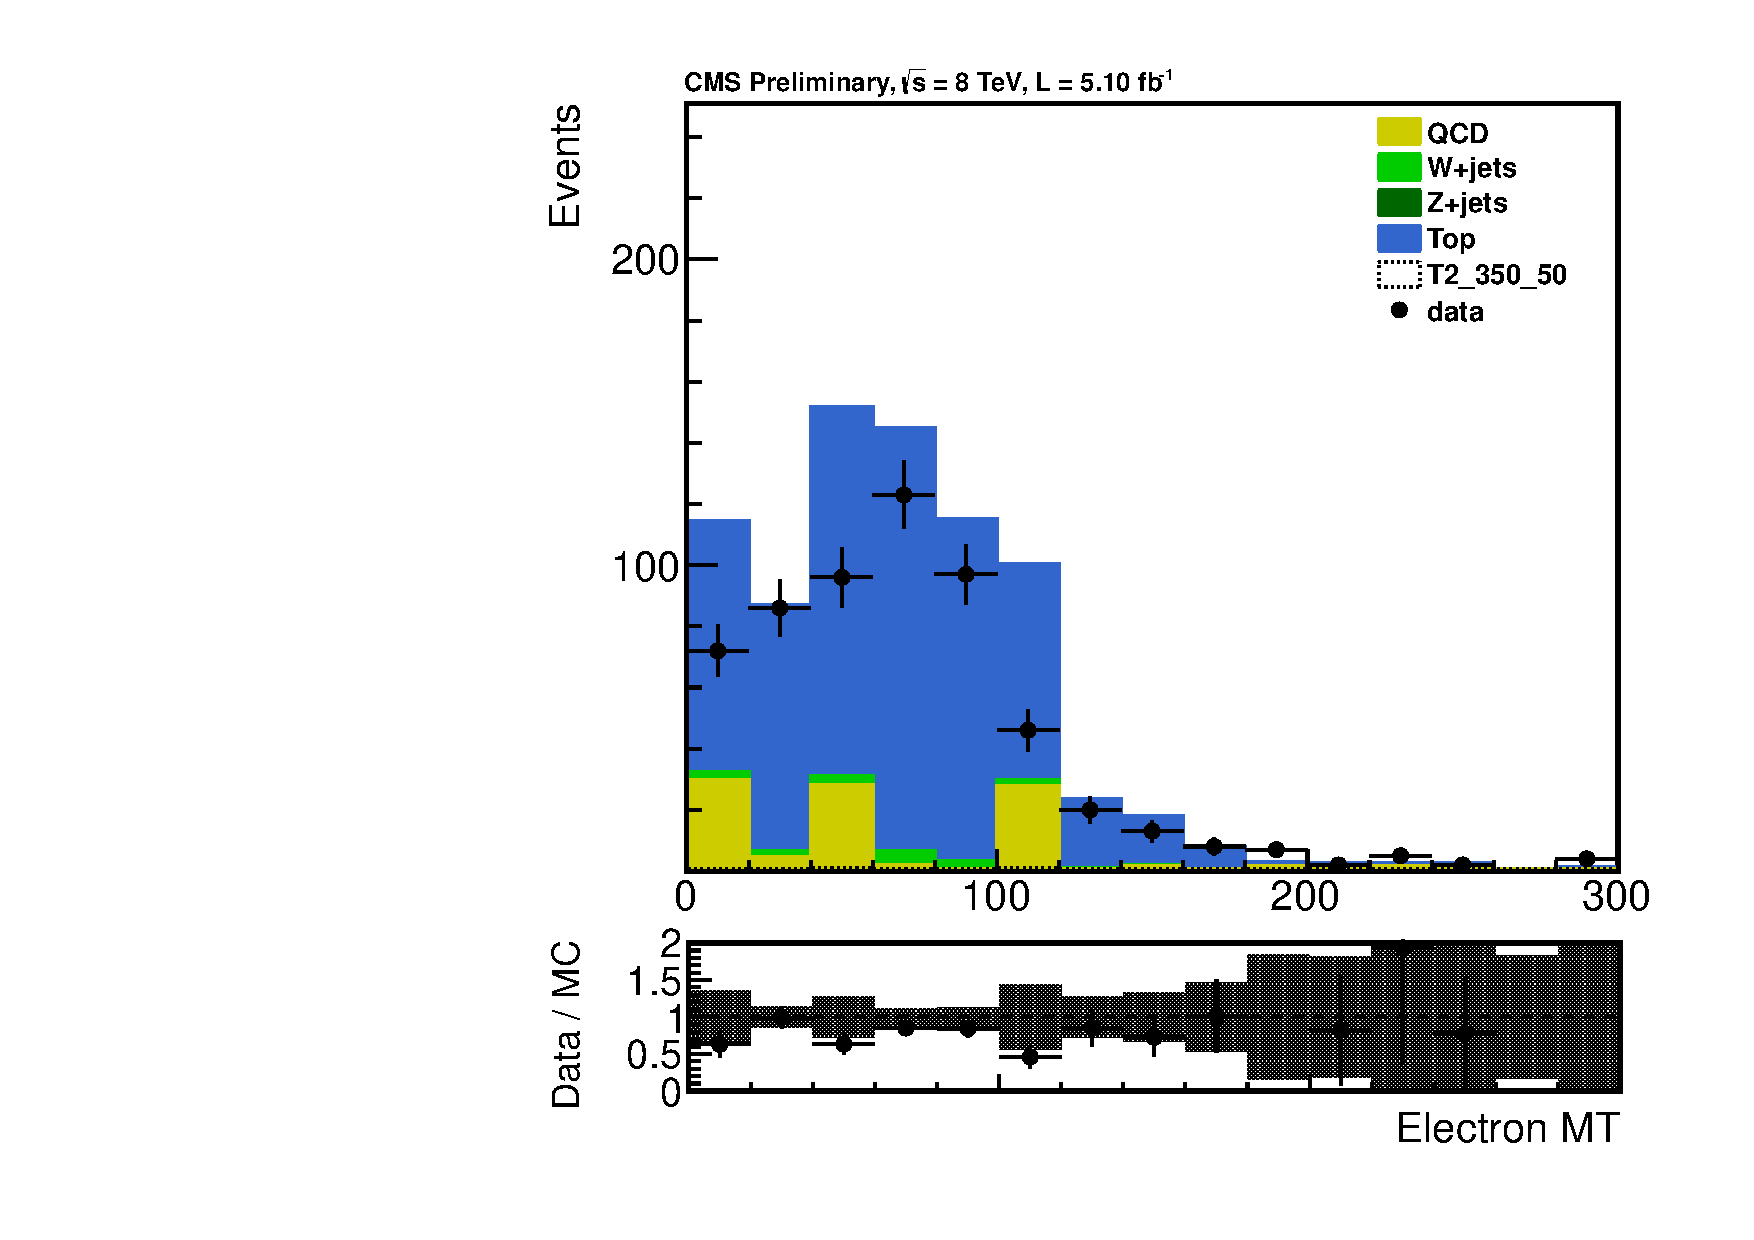
\includegraphics[angle=0,scale=0.39]{myplots/ele_mt.pdf} 
%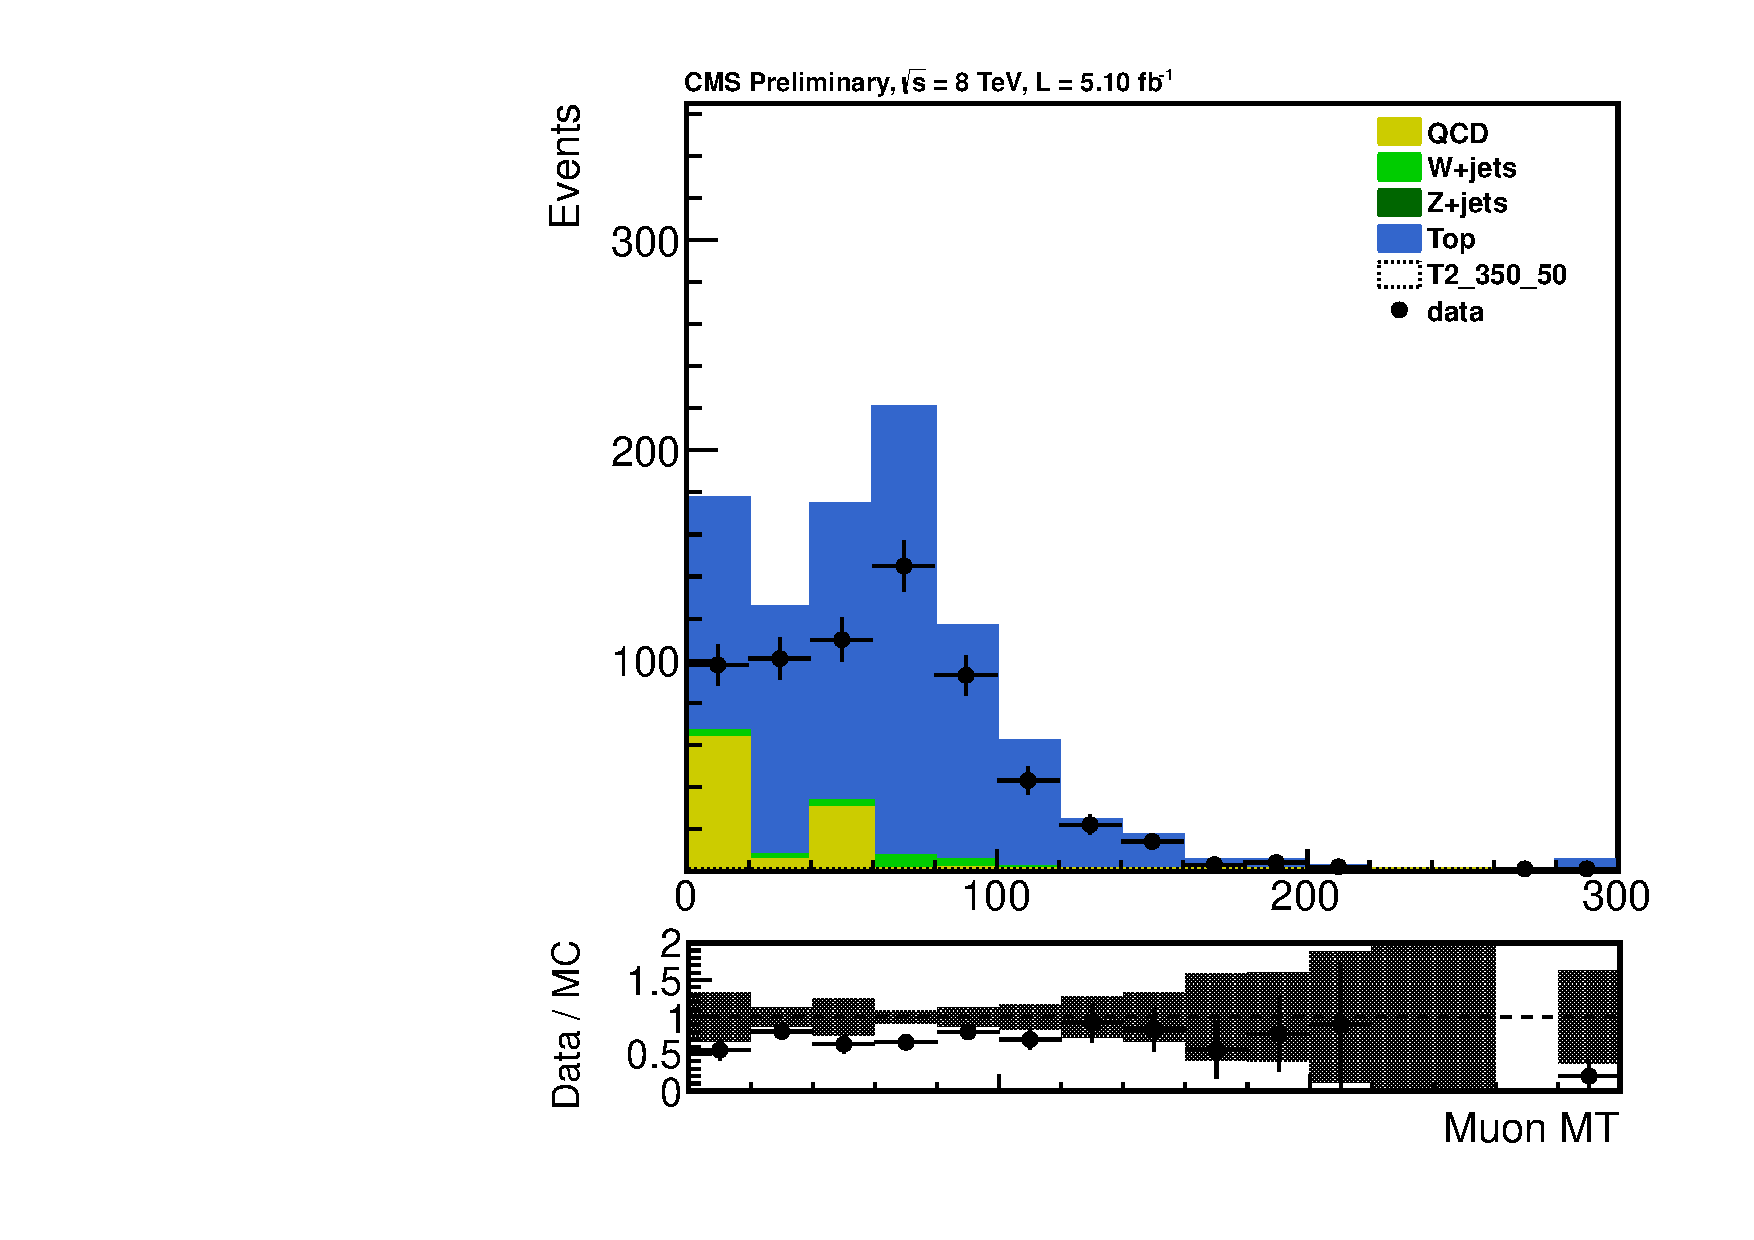
\includegraphics[angle=0,scale=0.39]{myplots/muo_mt.pdf} \\
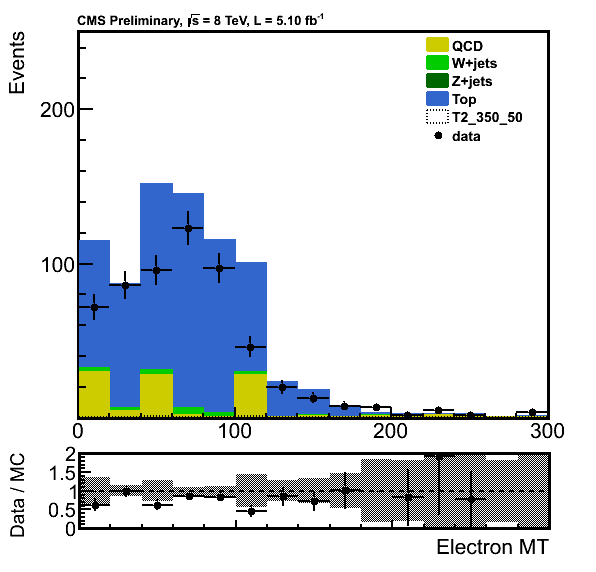
\includegraphics[angle=0,scale=0.35]{llplots_20Invfb/ele_mt.png} 
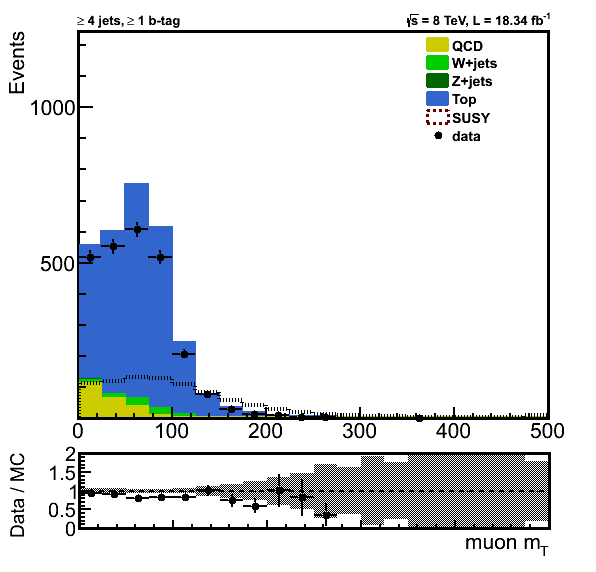
\includegraphics[angle=0,scale=0.35]{llplots_20Invfb/mu_mt.png} \\
\caption{Left: The $m_T$ distribution of the electrons for the events with one electron 
passing all selection cuts but the \mindphifour cut. The reason for this is stated in the text. No $M_{T2}$ cut is applied in 
order to have more statistics. Right: The same plot for muons.}
\label{fig:mt}
\end{figure}

The fraction of events with all selection cuts with respect to the events with all 
selection cuts but the \mindphifour are shown 
in Figure~\ref{fig:fraction} for data and MC. Since in the signal region, defined as region with $M_{T2}>125$ GeV, the ratios become flat; therefore one can fit the ratios with a straight line. For both electrons and muons, the MC ratio is fitted and the fitted parameters $f$ are quoted in Table~\ref{tbl:fitvalues}.\\
\begin{figure}[htbp] 
\centering
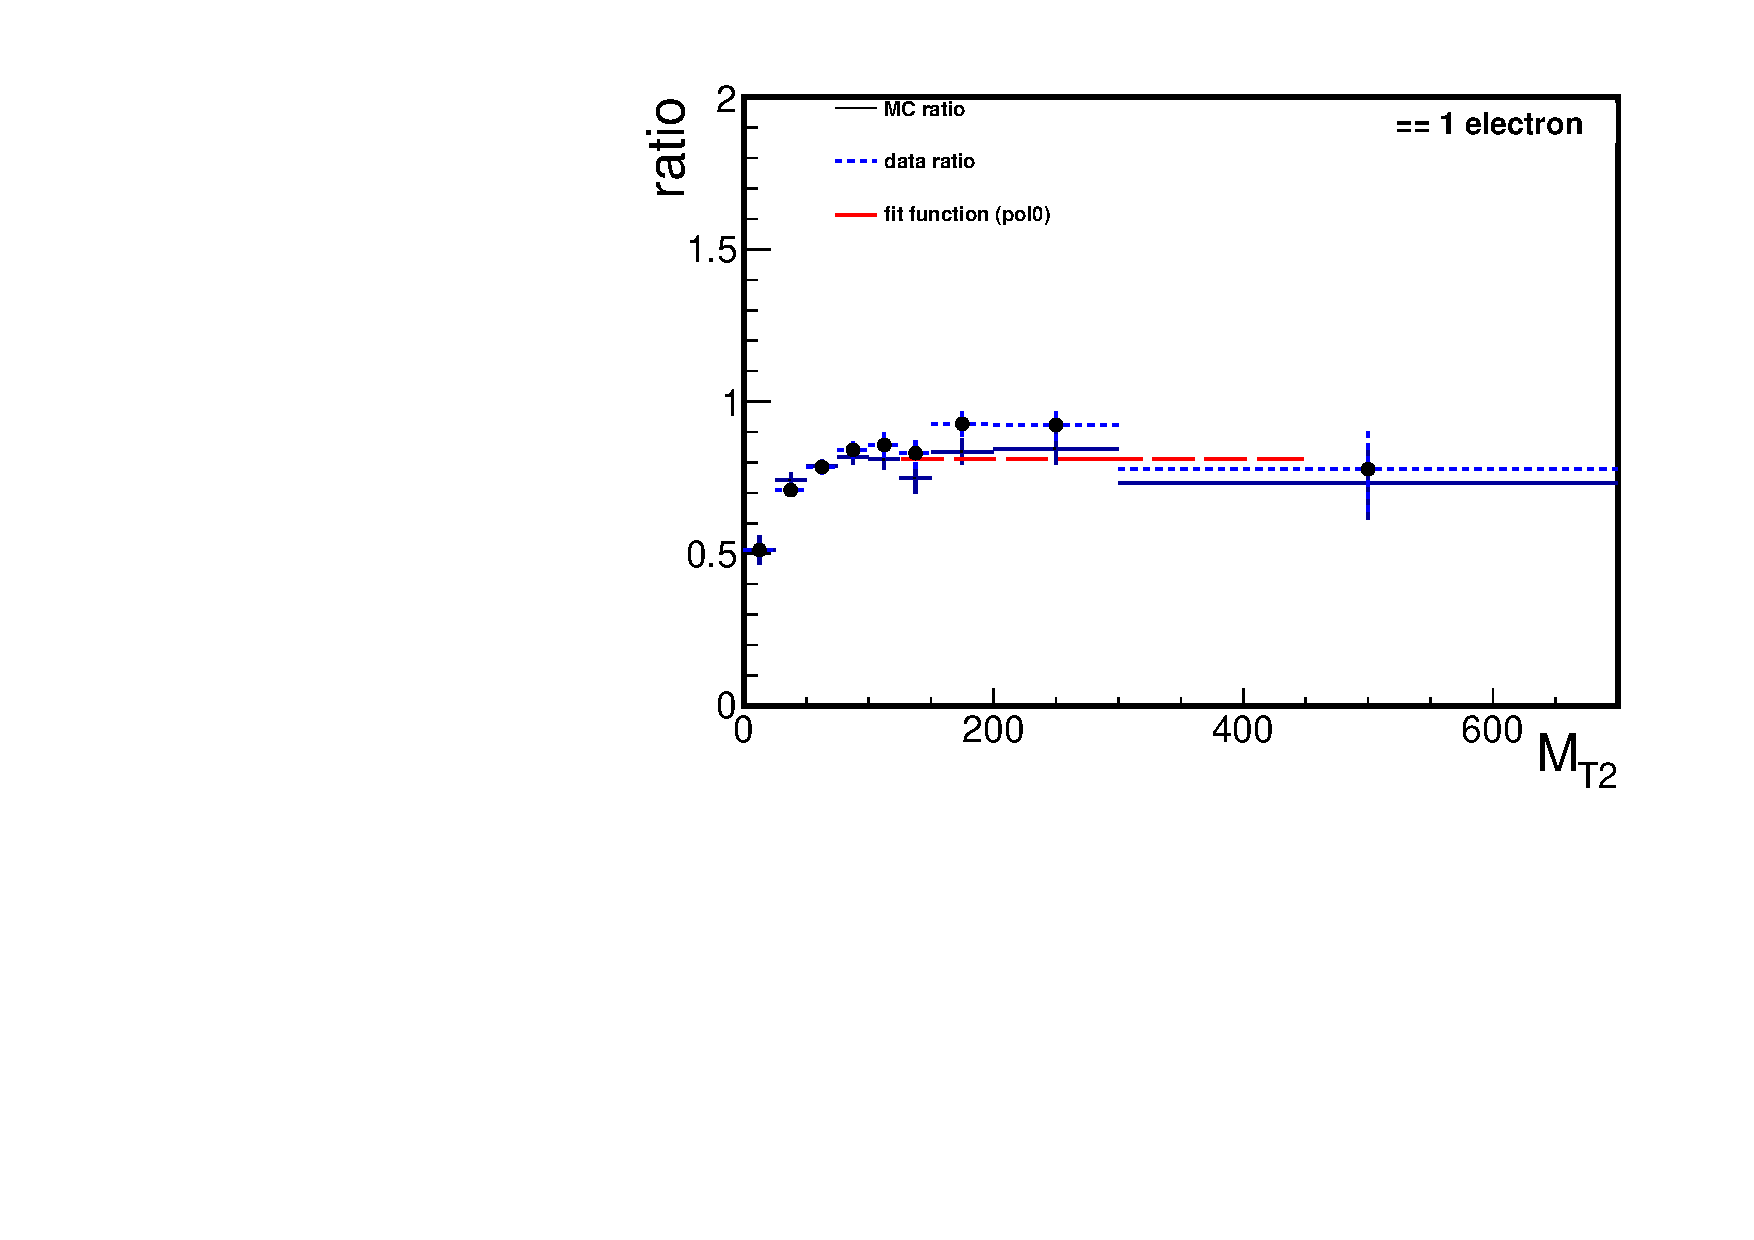
\includegraphics[angle=0,scale=0.39]{llplots_20Invfb/ele_ratio.pdf} 
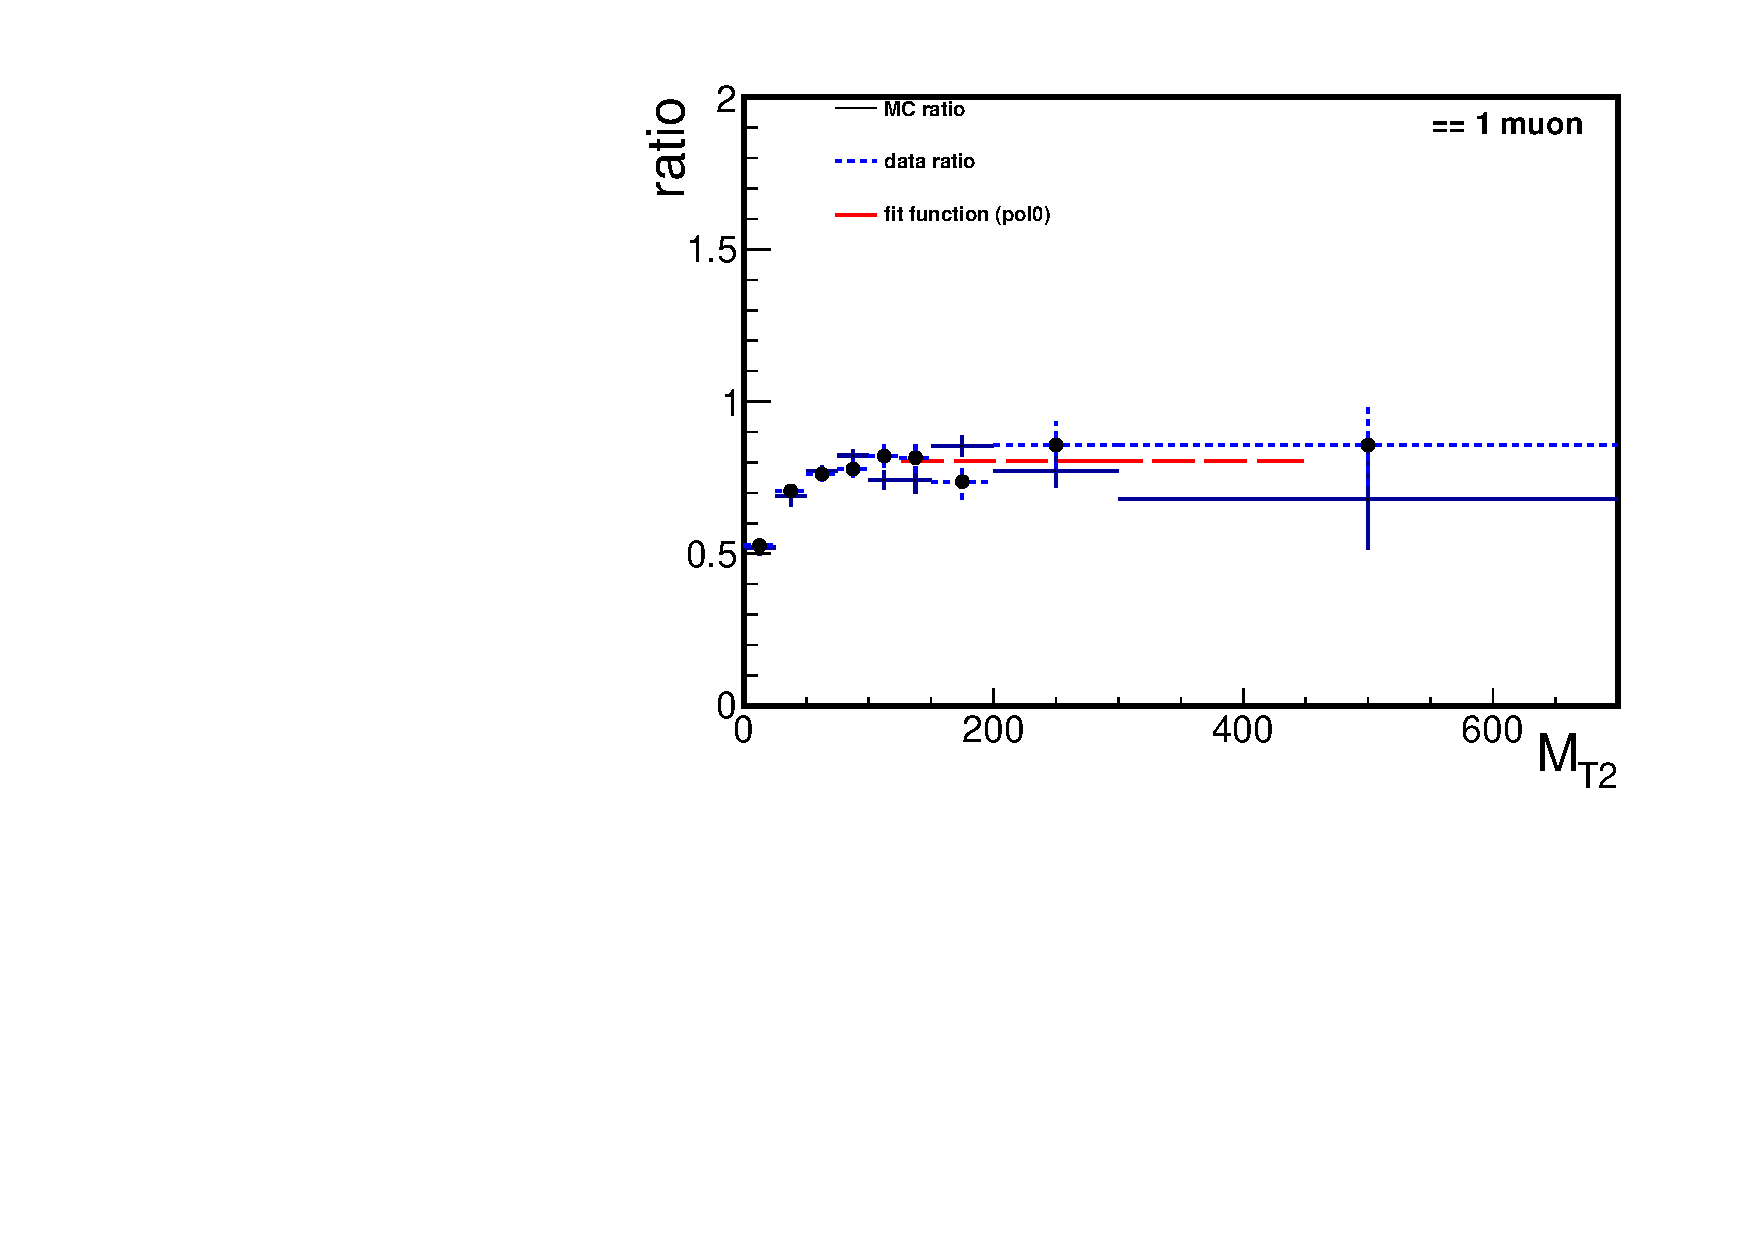
\includegraphics[angle=0,scale=0.39]{llplots_20Invfb/mu_ratio.pdf} \\
\caption{Left: Ratio between events with one electron passing all selection cuts 
versus events with one electron passing all selection cuts but the 
\mindphifour for data (blue) and MC (black). 
The fit line for the MC ratio over all $M_{T2}$ signal bins is drawn in red. Right: The same plot for events with one muon.}
\label{fig:fraction}
\end{figure}

\begin{table}[hbtp]
\begin{center}
\small
\begin{tabular}{lcc}\hline\hline
   &  electrons    &   muons   \\ \hline
Fit value for the ratio $f$    & $0.811 \pm 0.028$     &   $0.804 \pm 0.024$    \\ \hline\hline
\end{tabular}
\caption{Fit values $f$ obtained from the MC ratios for electrons and muons.}
\label{tbl:fitvalues}
\end{center}
\end{table}

The results of estimation of the lost lepton background events from data are summarized in 
Table~\ref{tbl:llestimation}. It should be mentioned that, the number of data events with 
one lepton selection and its corresponding background events are obtained from the relaxed 
cut selection, where \mindphifour is dropped. Therefore the prediction 
is corrected back by multiplying the event yield with the fitted ratio value $f$.\\ 
\begin{table}[hbtp]
\begin{center} 
\begin{tabular}{lccccc} 
\hline\hline 
& %$N^{W,Top}$ MC &
 $N^{reco}$ & $N^{bg}$ & $R_{LL}$ & $N^{pass}$ MC-Truth & $N^{pass}$ data-prediction \\\hline 
electrons &%&
&&&&\\\hline 
& %$38.94$ &
 $129$ & $20.78$ & $1.30\pm0.17$ & $189.32\pm10.86$ & $139.63\pm 14.72(stat)\pm 33.48 (sys)$\\\hline\hline 
muons &%&
&&&&\\\hline 
& %$45.55$ &
 $150$ & $25.42$ & $0.73\pm0.13$ & $133.08\pm 9.16$ & $91.29\pm 8.97 (stat)\pm 24.97 (sys)$\\ 
\hline\hline 
\end{tabular} 
\caption{Data-Driven Estimation of Lost Lepton from $W+$jets and $t(\bar t)$ for electrons and muons. The lost lepton ratio $R_{LL}$ is given by $f\frac{1-\varepsilon_l}{\varepsilon_l}$.}
\label{tbl:llestimation}
\end{center} 
\end{table} 

It should be noted that for the systematic uncertainty, two possible sources are taken into account. A first one is a systematic uncertainty of 100\% on the number of backgrounds. A second one is a systematic uncertainty of 5\%, considered when calculating the efficiencies $\varepsilon_l$ from MC, to account for possible difference between data and simulation.


\subsection{Estimation of the Tau Leptons}
\label{sect:tau}
Tau leptons can decay hadronically and appear as a thin jet and enter the hadronic searches. 
To estimate the contamination from such events a method similar to what is used for the lost lepton background is used here. The number of 
events with exactly one real tau is corrected by accounting for the reconstruction and acceptance efficiencies. In the other words:
\begin{linenomath}
\begin{equation}
	N_{W\rightarrow{\tau\nu}} = \frac{N_{\tau}^{reco} - N_{\tau}^{bg}}{\varepsilon_{\tau}},
	\label{eq:TauEstimation}
\end{equation}
\end{linenomath}
where $N_{\tau}^{reco}$ is the number of events with one reconstructed tau, $N_{\tau}^{bg}$ is the number of events with a 
fake tau and $\varepsilon_{\tau}$ denotes the probability for a generated
$W \rightarrow \tau\nu, \ \tau \to had$ event passing the selection cuts to have a reconstructed and identified tau. 
The efficiency $\varepsilon_{\tau}$ is extracted from simulation. In average, $\varepsilon_{\tau}$ is found to be $\sim24$\%. 5\% systematic 
uncertainty is assigned to this value to take into account the differences between data and MC.
The transverse mass (\mt) of the system of the reconstructed tau and MET is forced to be less than 100 GeV/$c^2$ to decrease 
the signal contamination.  The number of events with a fake tau, $N_{\tau}^{bg}$ is found from the MC simulation and a 50\% systematic 
uncertainty is assigned to this value.

The \mttwo distribution of the events with all selection cuts which have an
identified tau in the final state is shown in Figure \ref{fig:MT2Tau}.
\begin{figure}[!htb]
\centering
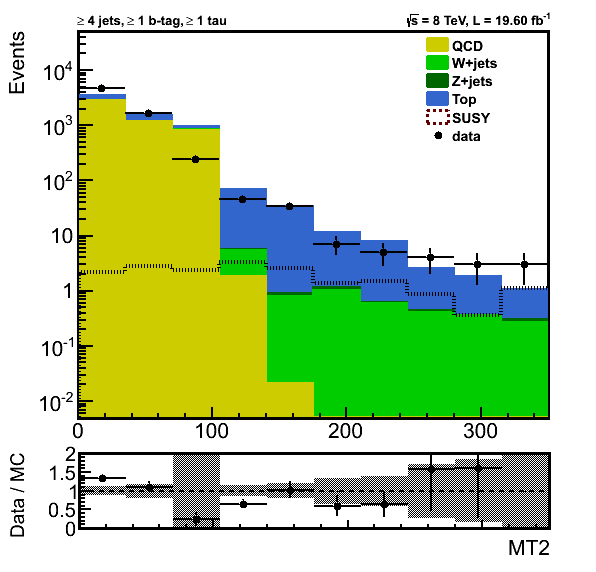
\includegraphics[width=0.49\textwidth]{figs/MT2Tau.png}
\caption{\mttwo distribution for events with at least one tau in data and MC with all selection cuts.}
\label{fig:MT2Tau}
\end{figure}
Scale factors of the tau selection are not applied and it can be the source of the discrepancies between data and MC. 
In Table~\ref{table:Tau_yield} 
\begin{table}[!htb]
\begin{center}
\small
\begin{tabular}{lcccccc}
\hline\hline
\mttwo (GeV)   &  QCD   & Z+Jets & W+Jets & Top & MC(sum) & data \\
\hline
 full range & 1480.06 & 0.35 & 9.59 & 417.80 & 1907.79 $\pm$ 182.88 & 2309.00\\
$125-\infty$ &   1.46 & 0.08 & 0.94 &  20.13 &   22.61 $\pm$ 4.57   & 21.00\\
\hline\hline
\multicolumn{7}{c}{cut on \mindphifour is relaxed}\\
\hline\hline
$125-\infty$ &      6.21 & 0.11 & 2.03 & 31.91 & 40.25 $\pm$ 6.18 & 34.00\\
\hline\hline
\end{tabular}
\caption{MC and data event yields in full range and signal region. The last row shows the yields after relaxing the cut.
The error on the total background is purely statistical.}
\label{table:Tau_yield}
\end{center}
\end{table}
contribution of different samples in the plot of Figure \ref{fig:MT2Tau} is shown. It can be seen that the statistics in the signal
region is poor. To decrease the uncertainties of the predictions, the cut on  \mindphifour is relaxed. 
The last row of the table shows the statistics after this relaxation. The scale factor to compensate this relaxation is 
read from MC.

Table \ref{table:MT2TauCutsRelaxed} 
\begin{table}[!htb]
\begin{center}
\small
\begin{tabular}{lccc}
\hline\hline
  \mttwo bin  &      MC Truth     &         Prediction in MC       & Prediction in Data \\\hline
$125-\infty$   &  78.40 $\pm$ 9.64 &  77.38 $\pm$ 19.94 $\pm$ 35.63 & 57.20 $\pm$ 18.83 $\pm$ 33.00\\
\hline\hline
\end{tabular}
\caption{Prediction of the tau contamination in the signal region in both data and MC.}
\label{table:MT2TauCutsRelaxed}
\end{center}
\end{table}
shows the performance of the method on MC and data. The quoted uncertainties of the predictions are statistical and systematical, respectively.

\subsection{Estimation of Invisible Z Background from Data Using W +jets Events}
\label{sect:znunu}
To estimate $Z\rightarrow\nu\bar{\nu}$ background we use $W\rightarrow\mu\nu$+jets events. The kinematics of leptons as well as the jets are very similar in both Z+jets and W+jets processes. Besides, the larger cross-section of W+jets allows for a more precise estimation of
$Z\rightarrow\nu\bar{\nu}$.  This is a well studied method in various analyses within the CMS Collaboration (see e.g. \cite{CMS-PAS-SUS-08-002,CMS-PAS-SUS-10-001,CMS-PAS-SUS-11-005}).
To make the event kinematics compatible from the \met point of view, the \pT of muon is added to the one of neutrino in W+jets events. The \mttwo variable and other quantities related to \met are recalculated accordingly.
This estimation can be described as:

\begin{linenomath}
\begin{equation}
\label{eq:ZinvEst}
N_{Z\rightarrow\nu\bar{\nu}}(est) = N_{W (\mu\nu)} R^{MC} \frac{1}{\epsilon_{acc}\epsilon_{reco/iso}}.
\end{equation}
\end{linenomath}
where,\\
$\bullet \hspace{5pt} \epsilon_{acc}$ is the muon acceptance derived from MC.\\
$\bullet \hspace{5pt} \epsilon_{reco/iso}$ is the muon reconstruction and isolation efficiency, taken from data using the Tag\&Probe method.\\
$\bullet \hspace{5pt} R^{MC}$ corrects kinematic, selection and cross-sections differences between $Z\rightarrow\nu\bar{\nu}$ and $W\rightarrow\mu\nu$+jets processes.\\
$\bullet \hspace{5pt} N_{W (\mu\nu)}$ is the number of selected $W\rightarrow\mu\nu$+jets events.\\

The selection is similar to the one of signal where the lepton veto is reduced to an electron veto. In addition we request for the presence of exactly one reconstructed muon passing all the quality and isolation cuts, with $p_T >10$ GeV and $|\eta| <2.4$. The W-boson transverse mass (using default \met) is required to be $\mt < 100$ GeV in order to reduce other backgrounds and signal contaminations. To enrich the sample with W+jets and to reject $t\bar{t}$ events, we veto events with at least one b-tagged jet where the medium working point of CSV b-tagging algorithm is applied on jets with $p_T >20$ and $|\eta| <2.4$. The results of this selection for MC samples and data are summarized in Table~\ref{tab:WenrichYields}. The distributions of muon \pT, \mttwo and \mt for this region are shown in Figures~\ref{fig:WenrichedPlots}a,~\ref{fig:WenrichedPlots}b and~\ref{fig:WenrichedPlots}c and as it is seen there is a good agreement between data and MC in W enriched region.\\
\begin{figure}[!h]
\begin{center}$
\begin{array}{cc} 
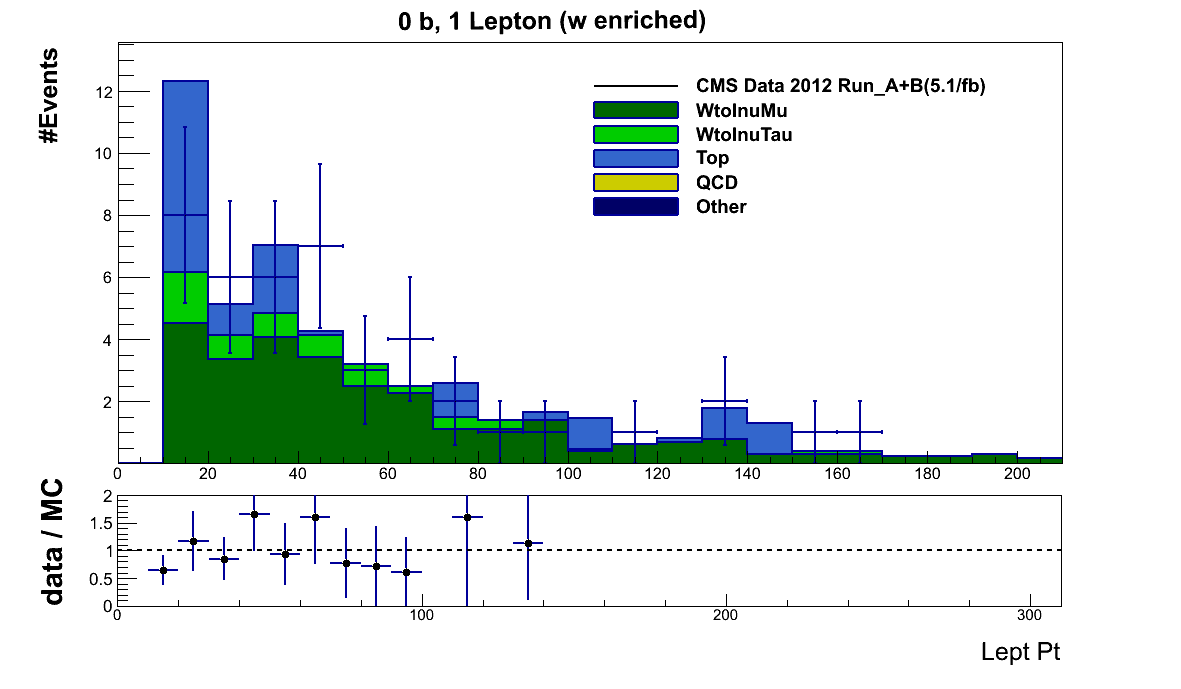
\includegraphics[angle=00,width=0.5\textwidth]{figs/Lept_Pt_0b_Mod.png}&
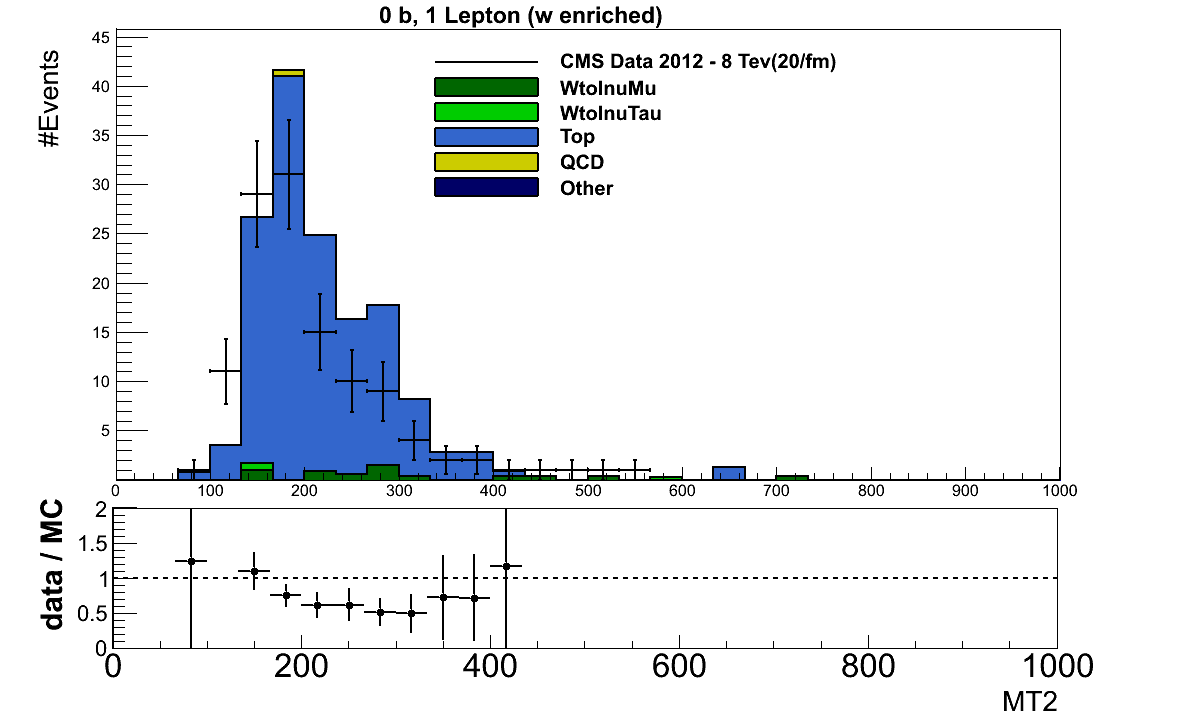
\includegraphics[angle=00,width=0.5\textwidth]{figs/MT2_0b_Mod.png}\\
	\mbox{\small{(a)}} & \mbox{\small{(b)}} \\
\end{array}$
\end{center}
\begin{center}$
\begin{array}{c}
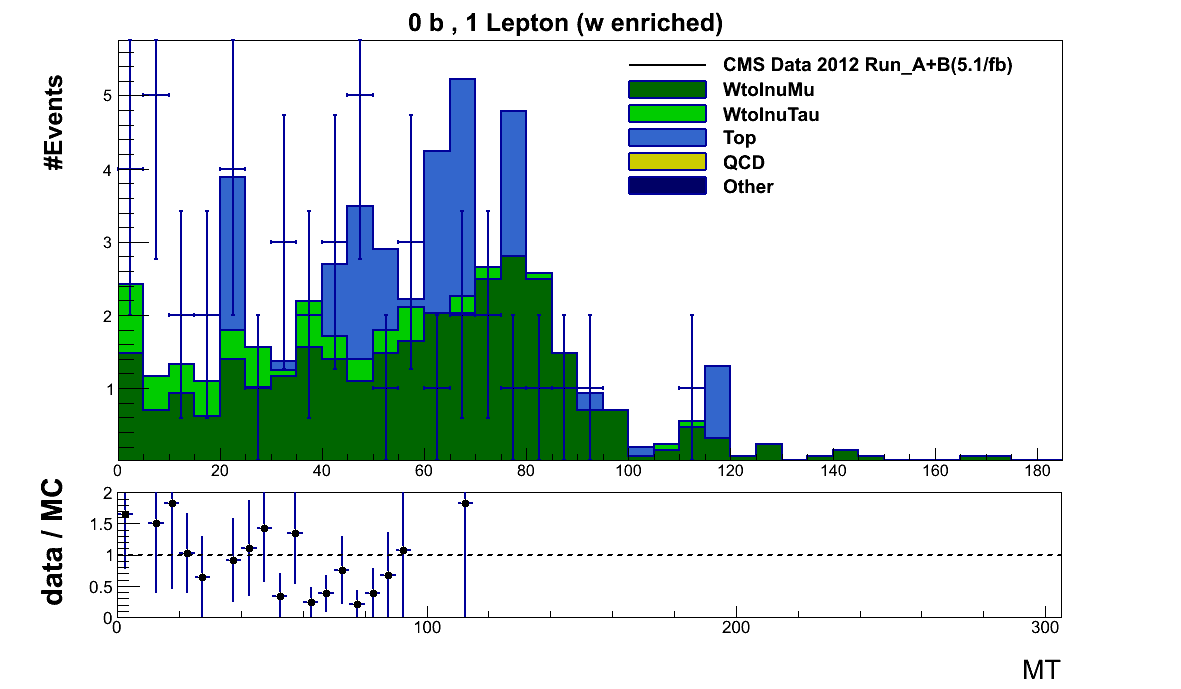
\includegraphics[angle=00,width=0.5\textwidth]{figs/MT_0b_Mod.png}\\
	\mbox{\small{(c)}}  \\
\end{array}$
\end{center}
\caption{Muon \pT, \mttwo and \mt distributions for W-enriched region}
\label{fig:WenrichedPlots}

\end{figure}


%..........................
\begin{table}[!htb]
\setlength{\tabcolsep}{2pt}
\small
\begin{center}

\begin{tabular}{lccccccccc} 
\hline\hline
& WtolnuMu& WtolnuTau& QCD& Zinv& Top& SMS& Other& MC& data \\ \hline \hline
 All events ($\rm jets\geq X$) & 145.81  & 230.75  & 462.23  & 235.41  & 1314.11  & 0.00 & 184.86  & 2573.17 +- 80.53 & 2510.00  \\
 %$Minimum DPhi(\met,jet) > 0.3$ & 40.56  & 65.36  & 146.80  & 65.29  & 328.56  & 0.06  & 50.78  & 697.35 $\pm$ 52.10 & 597.00  \\ 
 %HBHE noise veto & 40.56  & 65.36  & 146.80  & 65.29  & 328.56  & 0.06  & 50.78  & 697.35 $\pm$ 52.10 & 597.00  \\ 
 %$\met > 30GeV$ & 40.56  & 65.36  & 146.80  & 65.29  & 328.56  & 0.06  & 50.78  & 697.35 $\pm$ 52.10 & 597.00  \\ 
% $VectorSumPt < 70$ & 40.56  & 65.36  & 146.80  & 65.29  & 328.56  & 0.06  & 50.78  & 697.35 $\pm$ 52.10 & 597.00  \\ 
Analysis selection cuts& 145.81  & 230.75  & 462.23  & 235.41  & 1314.11  & 0.00 & 184.86  & 2573.17 +- 80.53 & 2510.00  \\ 
Lepton Veto & 145.81  & 214.43  & 459.75  & 235.29  & 1068.30  & 0.00 & 96.65  & 2220.23 +- 78.92 & 2192.00  \\ 
Lepton Selection & 91.76  & 17.61  & 0.74  & 0.11  & 277.43  & 0.00 & 6.00  & 393.65 +- 16.96 & 329.00  \\ 
$m_T < 100\, \rm GeV$ & 83.26  & 17.30  & 0.74  & 0.06  & 241.95  & 0.00 & 6.00  & 349.30 +- 15.99 & 293.00  \\  
$b$-jets Selection & 69.67  & 15.29  & 0.00  & 0.03  & 27.85  & 0.00 & 6.00  & 118.83 +- 8.25 & 130.00  \\ 
 \mttwo  100 - 150 GeV & 8.97  & 1.56  & 0.00  & 0.00  & 4.67  & 0.00  & 0.00  & 15.20 +- 2.69 & 12.00  \\ 
 \mttwo  150 - 200 GeV & 19.28  & 4.94  & 0.00  & 0.03  & 6.61  & 0.00 & 0.00  & 30.86 +- 3.67 & 44.00  \\
 \mttwo  200 - 275 GeV & 19.45  & 4.09  & 0.00  & 0.00  & 8.71  & 0.00 & 2.88  & 35.14 +- 4.75 & 41.00  \\ 
 \mttwo  275 - 375 GeV  & 9.80  & 2.25  & 0.00  & 0.00  & 4.19  & 0.00 & 0.00  & 16.24 +- 2.71 & 21.00  \\ 
 \mttwo  375 - 500 GeV & 7.39  & 2.08  & 0.00  & 0.00  & 2.57  & 0.00 & 0.00  & 12.04 +- 2.33 & 7.00  \\ 
 $\mttwo > 500$ GeV & 4.08  & 0.37  & 0.00  & 0.00  & 1.10  & 0.00  & 3.12  & 8.67 +- 3.43 & 5.00  \\
\hline\hline 
\end{tabular} 
\caption{Yields for the W-enriched selection}
\label{tab:WenrichYields}
\end{center} 
\end{table}
%..........xxx ����..
\begin{table}
\begin{center}
\begin{tabular}{lcccccccccccccccc}
\hline\hline
& WtolnuMu& WtolnuTau& QCD& Zinv& Top& SUSY& Other& MC& data \\ \hline \hline
 All events(jets >= X) & 136.44  & 215.93  & 569.94  & 220.29  & 1300.06  & 0.00  & 172.98  & 2615.64 +- 61.07 & 2510.00  \\
 Minimum DPhi(MET,jet) > 0.3 & 136.44  & 215.93  & 569.94  & 220.29  & 1300.06  & 0.00  & 172.98  & 2615.64 +- 61.07 & 2510.00  \\
 HBHE noise veto & 136.44  & 215.93  & 569.94  & 220.29  & 1300.06  & 0.00  & 172.98  & 2615.64 +- 61.07 & 2510.00  \\
 MET > 30 GeV & 136.44  & 215.93  & 569.94  & 220.29  & 1300.06  & 0.00  & 172.98  & 2615.64 +- 61.07 & 2510.00  \\
 VectorSumPt < 70 & 136.44  & 215.93  & 569.94  & 220.29  & 1300.06  & 0.00  & 172.98  & 2615.64 +- 61.07 & 2510.00  \\
 jets > 50GeV failing PFID event veto & 136.44  & 215.93  & 569.94  & 220.29  & 1300.06  & 0.00  & 172.98  & 2615.64 +- 61.07 & 2510.00  \\
 Lepton Veto & 136.44  & 200.65  & 569.33  & 220.18  & 1056.97  & 0.00  & 90.44  & 2274.01 +- 59.24 & 2192.00  \\
 Lepton Selection & 85.86  & 16.48  & 0.00  & 0.11  & 273.96  & 0.00  & 5.62  & 382.03 +- 15.87 & 329.00  \\
 MT < 100 & 77.91  & 16.19  & 0.00  & 0.06  & 238.63  & 0.00  & 5.62  & 338.40 +- 14.96 & 293.00  \\
 BJets & 65.19  & 14.31  & 0.00  & 0.03  & 27.55  & 0.00  & 5.62  & 112.69 +- 7.72 & 130.00  \\
 MT2  100 - 150 GeV & 8.40  & 1.46  & 0.00  & 0.00  & 4.67  & 0.00  & 0.00  & 14.53 +- 2.52 & 12.00  \\
 MT2  150 - 200 GeV & 18.04  & 4.62  & 0.00  & 0.03  & 6.73  & 0.00  & 0.00  & 29.43 +- 3.43 & 44.00  \\
 MT2  200 - 275 GeV & 18.20  & 3.83  & 0.00  & 0.00  & 8.45  & 0.00  & 2.70  & 33.18 +- 4.45 & 41.00  \\
 MT2  275 - 375 GeV & 9.17  & 2.10  & 0.00  & 0.00  & 4.14  & 0.00  & 0.00  & 15.41 +- 2.54 & 21.00  \\
 MT2  375 - 500 GeV & 6.92  & 1.95  & 0.00  & 0.00  & 2.49  & 0.00  & 0.00  & 11.36 +- 2.18 & 7.00  \\
 MT2 > 500 GeV & 3.82  & 0.34  & 0.00  & 0.00  & 1.06  & 0.00  & 2.92  & 8.15 +- 3.21 & 5.00  \\
\hline\hline
\end{tabular}
\end{center}
\end{table}

\subsubsection{\texorpdfstring{$\rm{t\bar{t}}$ background estimation in W-enriched sample}{tt background estimation in W-enriched sample}}

Despite of b-tag veto some top events remain in W enriched region. The contribution of $t\bar{t}$ is estimated from data while for the rest of backgrounds we trust on simulation. The b-tag veto is relaxed and at least one b-jet is requested to obtain a sample enriched in top events. The selection results are shown in Table~\ref{tab:toEnrichyields}. To find out the number top events in b-tag veto region (W enriched), b-tagging (in)efficiency has to be considered. This process can be described as:
%.................
\begin{linenomath}
\begin{equation}
\label{eq:topEst}
N_{top}(b-veto) = N_{top}(\geq1b-tag) \frac{\epsilon(b-veto)}{\epsilon(\geq1b-tag)},
\end{equation}
\end{linenomath}
where the $\epsilon(b-veto)$ and $\epsilon(\geq1b-tag)$ are the efficiencies of vetoing or selecting b-tagged events and are taken from simulation, thus corrected by the data-simulation scale factors given by the b-tag POG for the CSVE (0.963 $\pm$ 0.020) and CSVT(0.947 $\pm$ 0.025) working points, respectively~\cite{CMS-BTV-AN-12-470}. As it is apparent from Table~\ref{tab:toEnrichyields} there is a good agreement between data and MC in top-enriched region and also the Muon \pT, \mttwo and \mt distributions are shown in Figures~\ref{fig:topEnrichedPlots}a,~\ref{fig:topEnrichedPlots}b and~\ref{fig:topEnrichedPlots}c, respectively.


\begin{figure}[!h]
\begin{center}$
\begin{array}{cc} 
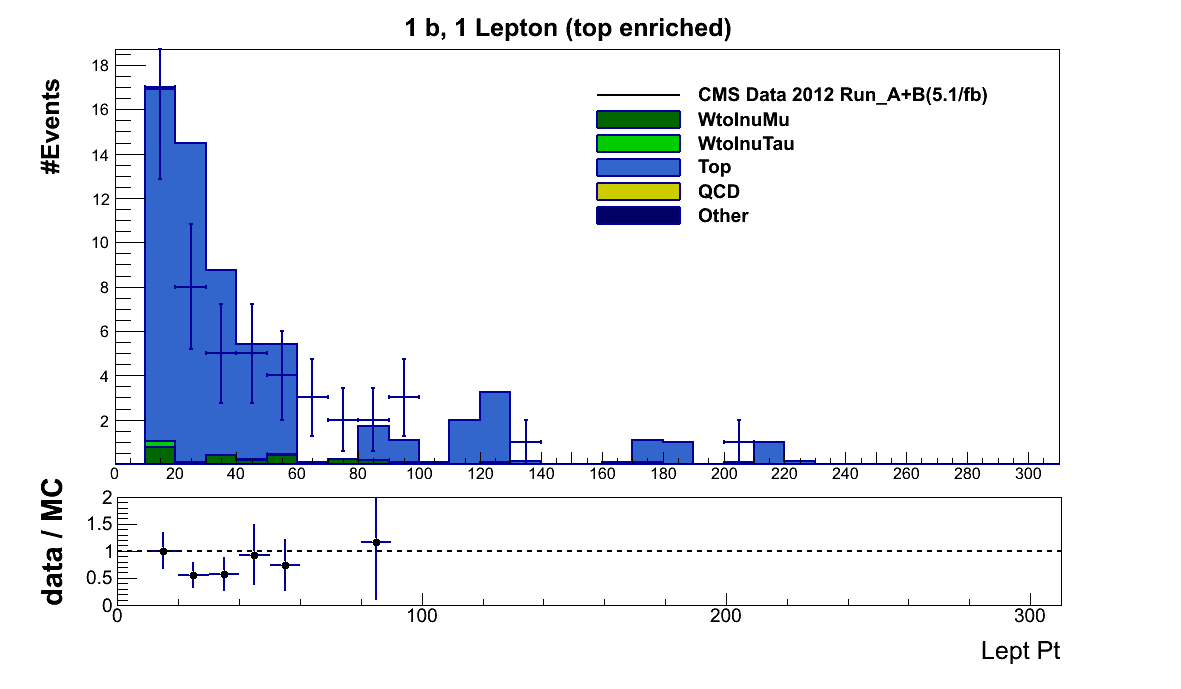
\includegraphics[angle=00,width=0.5\textwidth]{figs/Lept_Pt_1b_Mod.png}&
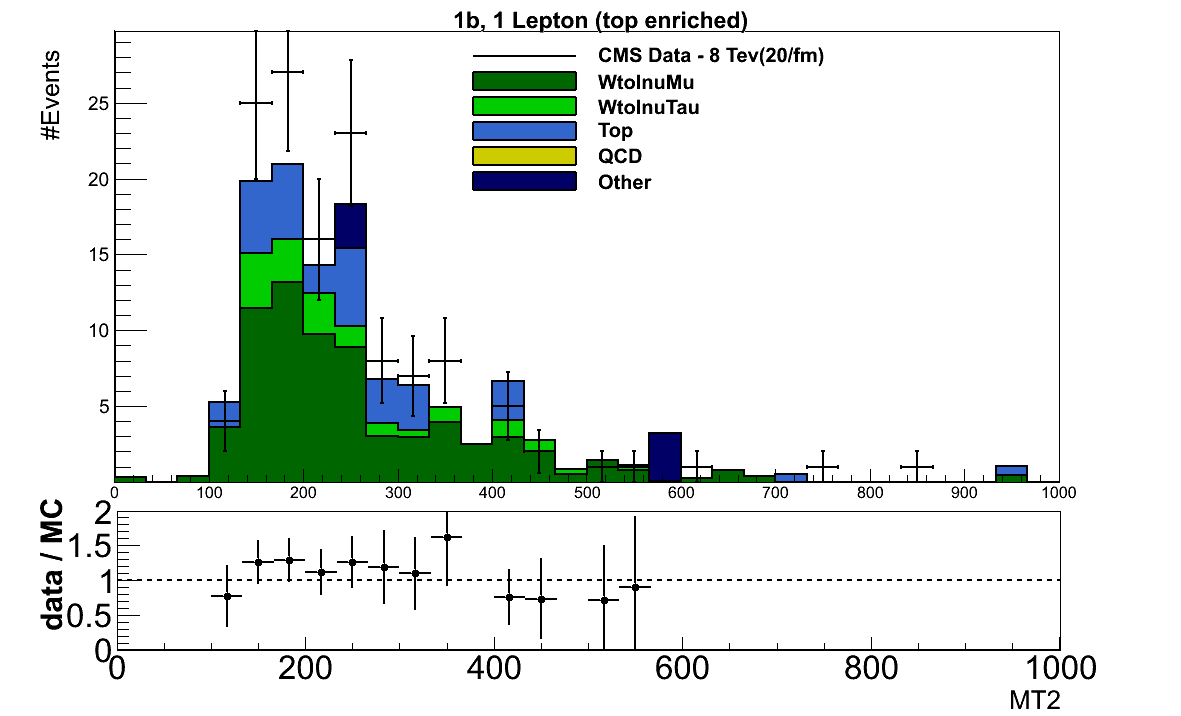
\includegraphics[angle=00,width=0.5\textwidth]{figs/MT2_1b_Mod.png}\\
	\mbox{\small{(a)}} & \mbox{\small{(b)}} \\
\end{array}$
\end{center}
\begin{center}$
\begin{array}{c}
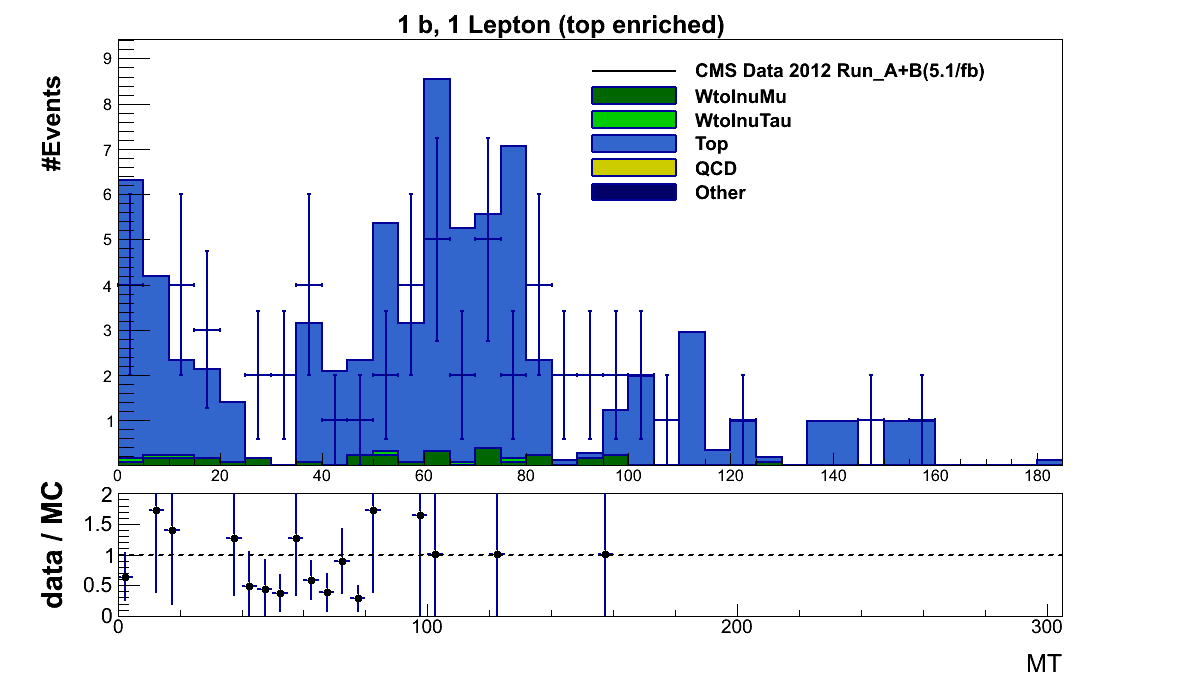
\includegraphics[angle=00,width=0.5\textwidth]{figs/MT_1b_Mod.png}\\
	\mbox{\small{(c)}}  \\
\end{array}$
\end{center}
\caption{Muon \pT, \mttwo and \mt distributions for top-enriched region}
\label{fig:topEnrichedPlots}
\end{figure}

%.....................
\begin{table}[!htb]
\setlength{\tabcolsep}{2pt}
\small
\begin{center} 

\begin{tabular}{lccccccccc} 
\hline\hline
& WtolnuMu& WtolnuTau& QCD& Zinv& Top& SMS& Other& MC& data \\ \hline \hline
 All events ($\rm jets\geq X$) & 170.32  & 267.04  & 493.27  & 270.57  & 1122.03  & 0.00 & 211.59  & 2534.83 +- 86.48 & 2510.00  \\ 
 %$Minimum DPhi(\met,jet) > 0.3$ & 40.56  & 65.36  & 146.80  & 65.29  & 328.56  & 0.06  & 50.78  & 697.35 $\pm$ 52.10 & 597.00  \\ 
 %HBHE noise veto & 40.56  & 65.36  & 146.80  & 65.29  & 328.56  & 0.06  & 50.78  & 697.35 $\pm$ 52.10 & 597.00  \\ 
 %$\met > 30GeV$ & 40.56  & 65.36  & 146.80  & 65.29  & 328.56  & 0.06  & 50.78  & 697.35 $\pm$ 52.10 & 597.00  \\ 
% $VectorSumPt < 70$ & 40.56  & 65.36  & 146.80  & 65.29  & 328.56  & 0.06  & 50.78  & 697.35 $\pm$ 52.10 & 597.00  \\ 
Analysis selection cuts & 170.32  & 267.04  & 493.27  & 270.57  & 1122.03  & 0.00 & 211.59  & 2534.83 +- 86.48 & 2510.00  \\ 

Lepton Veto & 170.32  & 248.45  & 490.77  & 270.43  & 913.06  & 0.00 & 109.45  & 2202.48 +- 85.20 & 2192.00  \\ 
Lepton Selection & 107.15  & 20.76  & 0.62  & 0.12  & 236.72  & 0.00 & 5.85  & 371.23 +- 15.38 & 329.00  \\ 
$m_T < 100\, \rm GeV$ & 97.37  & 20.36  & 0.62  & 0.06  & 206.08  & 0.00 & 5.85  & 330.34 +- 14.53 & 293.00  \\
$b$-jets Selection & 5.71  & 1.06  & 0.61  & 0.00  & 141.35  & 0.00 & 0.00  & 148.74 +- 10.24 & 119.00  \\  
\mttwo  100 - 150 GeV & 0.64  & 0.41  & 0.00  & 0.00  & 16.11  & 0.00 & 0.00  & 17.16 +- 3.47 & 28.00  \\ 
\mttwo  150 - 200 GeV & 0.31  & 0.34  & 0.61  & 0.00  & 53.26  & 0.00 & 0.00  & 54.53 +- 6.38 & 43.00  \\ 
\mttwo  200 - 275 GeV & 1.46  & 0.00  & 0.00  & 0.00  & 43.72  & 0.00 & 0.00  & 45.18 +- 5.64 & 26.00  \\ 
\mttwo  275 - 375 GeV & 1.94  & 0.00  & 0.00  & 0.00  & 24.37  & 0.00 & 0.00  & 26.30 +- 4.14 & 16.00  \\ 
\mttwo  375 - 500 GeV & 0.68  & 0.00  & 0.00  & 0.00  & 1.79  & 0.00 & 0.00  & 2.47 +- 1.17 & 3.00  \\ 
$\mttwo > 500 GeV$ & 0.69  & 0.30  & 0.00  & 0.00  & 1.30  & 0.00  & 0.00  & 2.29 +- 1.10 & 2.00  \\
\hline\hline 
\end{tabular} 
\caption{Yields for the top-enriched selection}
\label{tab:toEnrichyields}
\end{center} 
\end{table}
%............xxx�����
\begin{table}
\begin{center}
\begin{tabular}{lcccccccccccccccc}
\hline\hline
& WtolnuMu& WtolnuTau& QCD& Zinv& Top& SUSY& Other& MC& data \\ \hline \hline
 All events(jets >= X) & 159.38  & 249.89  & 593.54  & 253.19  & 1109.83  & 0.00  & 198.00  & 2563.82 +- 61.63 & 2510.00  \\
 Minimum DPhi(MET,jet) > 0.3 & 159.38  & 249.89  & 593.54  & 253.19  & 1109.83  & 0.00  & 198.00  & 2563.82 +- 61.63 & 2510.00  \\
 HBHE noise veto & 159.38  & 249.89  & 593.54  & 253.19  & 1109.83  & 0.00  & 198.00  & 2563.82 +- 61.63 & 2510.00  \\
 MET > 30 GeV & 159.38  & 249.89  & 593.54  & 253.19  & 1109.83  & 0.00  & 198.00  & 2563.82 +- 61.63 & 2510.00  \\
 VectorSumPt < 70 & 159.38  & 249.89  & 593.54  & 253.19  & 1109.83  & 0.00  & 198.00  & 2563.82 +- 61.63 & 2510.00  \\
 jets > 50GeV failing PFID event veto & 159.38  & 249.89  & 593.54  & 253.19  & 1109.83  & 0.00  & 198.00  & 2563.82 +- 61.63 & 2510.00  \\
 Lepton Veto & 159.38  & 232.49  & 593.04  & 253.06  & 903.14  & 0.00  & 102.42  & 2243.53 +- 60.09 & 2192.00  \\
 Lepton Selection & 100.27  & 19.43  & 0.00  & 0.12  & 233.72  & 0.00  & 5.48  & 359.01 +- 14.39 & 329.00  \\
 MT < 100 & 91.11  & 19.05  & 0.00  & 0.06  & 203.23  & 0.00  & 5.48  & 318.94 +- 13.59 & 293.00  \\
 BJets & 5.35  & 0.99  & 0.00  & 0.00  & 139.18  & 0.00  & 0.00  & 145.51 +- 9.57 & 119.00  \\
 MT2  100 - 150 GeV & 0.59  & 0.39  & 0.00  & 0.00  & 15.93  & 0.00  & 0.00  & 16.91 +- 3.25 & 28.00  \\
 MT2  150 - 200 GeV & 0.29  & 0.32  & 0.00  & 0.00  & 52.16  & 0.00  & 0.00  & 52.77 +- 5.94 & 43.00  \\
 MT2  200 - 275 GeV & 1.37  & 0.00  & 0.00  & 0.00  & 43.02  & 0.00  & 0.00  & 44.39 +- 5.28 & 26.00  \\
 MT2  275 - 375 GeV & 1.81  & 0.00  & 0.00  & 0.00  & 23.92  & 0.00  & 0.00  & 25.73 +- 3.88 & 16.00  \\
 MT2  375 - 500 GeV & 0.63  & 0.00  & 0.00  & 0.00  & 2.05  & 0.00  & 0.00  & 2.68 +- 1.10 & 3.00  \\
 MT2 > 500 GeV & 0.65  & 0.28  & 0.00  & 0.00  & 1.30  & 0.00  & 0.00  & 2.23 +- 1.03 & 2.00  \\
\hline\hline
\end{tabular}
\end{center}
\end{table}
%...........................
\subsubsection{Z Estimation Results}
After finding the number of top events in the b-tag veto (W-enriched) region, it is subtracted from the number of W's of this region, derived from data, to obtain the correct number of $W\rightarrow\mu\nu$ events. Due to requesting one b-jet in the final state we need to have the number of W's in 1 b-tag region to be able to estimate the number of Z in this region. Therefore we must multiply the number of W's in b-tag veto region to $\frac{\epsilon(1b W)}{\epsilon(0b W)}$ to reach the number of W's in 1 b-tag region and this ratio is coming from MC and it is considered b-tag scale factor.   

\subsubsection{Systematic uncertainties}
\label{subsect:ZnnSyst}
The systematic uncertainty on $Z\to \nu\nu$ estimation has contributions from different sources, as can be seen in Equation~\ref{eq:ZinvEst}. There, the uncertainty on $R^{MC}$ is taken from simulation where it includes the uncertainties due to the PDF set and the k-factor [FIXME?] in Z and W bosons production rates. The uncertaintiy on the muon acceptance efficiency is derived from simulation, too. The muon selection efficiency ($\epsilon_{reco/iso}$) as well as its uncertainty are data-driven, obtained from the Tag\&Probe method. Another uncertainty in this estimation arises from the requirement of $m_T<100\,\rm GeV$ which is estimated from simulation.\\
For the $N_{W(\mu\nu)}$ in the analysis region with at least one b-tagged jet, the $N_{W(\mu\nu)}$ estimation in b-tag veto region is corrected with  the data-driven b-tagging and b-tag veto efficiencies. The uncertainties on these efficiencies are taken from data, accordingly.\\
Other than $t\bar{t}$, all backgrounds and their uncertainties are estimated from simulation in $N_{W(\mu\nu)}$ calculation. The $t\bar{t}$ contribution in W-enriched (b-tag veto) region is obtained using Equation~\ref{eq:topEst}. In this estimation, the uncertainties on b-tagging efficiencies are taken from data while the background uncertanties are derived from simulation. \\ 

The final estimation together with their uncertainties are summarized in Table~\ref{tab:ZinvFinalRes}.

\begin{table}[!htb]
\small
\setlength{\tabcolsep}{20pt} 
\begin{center} 
\begin{tabular}{lccccccc} 
\hline\hline
&                 &    MC                     & Data Estimation\\\hline \hline
& top  (0b, 1l)     & 27.85 $\pm$ 4.68             &18.73 $\pm$ 4.56 ( 1.72 (stat) $\pm$4.22 (syst) )\\
&  W   (0b, 1l)     & 69.67 $\pm$ 4.79            & 89.98 $\pm$ 13.71 ( 8.08 (stat) $\pm$ 11.08 (syst))\\ 
& Zinv (1b, 0l)           &  22.74 $\pm$ 0.84            &19.68 $\pm$ 8.09 ( 1.77 (stat) $\pm$7.89 (syst))\\

%| | *Top est (0b, 1l)* | *Top MC (0b, 1l)* | *WJets est (0b, 1l)* | %*WJets MC (0b,1l)* | *ZInv est* | *ZInv MC* |
%| *MT2 [-1, 9999)* | 18.99 +- 4.44 ( 1.74 (stat) +- 4.08 (syst) ) | %27.55 +- 4.38 |  91.08 +- 13.69 ( 8.18 (stat) +- 10.99 (syst) ) |  65.19 %+- 4.49 |  19.92 +- 7.96 ( 1.79 (stat) +- 7.75 (syst) ) | 21.28 +- 0.79 %|

\hline\hline 
\end{tabular} 
\caption{Z-invisible Estimation}
\label{tab:ZinvFinalRes}
\end{center} 
\end{table}



\section[Statistics]{Statistical Interpretation of the results}\label{sect:stat}

\newcommand{\PSGcpmDo}{\ensuremath{\widetilde{\chi}_{1}^{\pm}}\xspace}


Since no excess of data over the background prediction has been observed, 
we close our study with setting upper limits on the testing signals.
This is conducted using a modified frequentist approach, namely CLs method \cite{read:CLs}.
In this method, the test statistic $q_\mu$ \cite{cowan:asymptoticCLs} is a function of the profile likelihood-ratio,

\begin{align}
q_\mu = -2 \ln \frac{\mathcal{L}(data ;\, b + \mu s)}{\mathcal{L}(data ;\, b + \hat{\mu} s)},
\end{align}

where $\hat\mu$ is the \textit{signal strength modifier} $\mu$ at the maximum point of the likelihood $\mathcal{L}$.
Then CLs is given by the following probability-ratio,

\begin{align}
CL_s = \frac{p(q_\mu \geq q_\mu^{obs} | b + \mu s )}{p(q_\mu \geq q_\mu^{obs} | b)}.
\end{align}
 
We compute CLs using a software package provided by the CMS Higgs PAG \cite{higgspag:software}.
After incorporating systematic uncertainties, an observed CLs smaller than 0.05 for a signal strength of $\mu = 1$, excludes the given signal at $95\%$ CL. Indeed, the package determines which signal strength $\mu$ excludes the testing signal at $95\%$ CL. Therefore all resulting $\mu \leq 1$ define the excluded region in the parameter space of the given signal. 


To investigate the exclusion power of our research, we study the topology of direct stau pair production and the $\PSGcpDo\PSGcmDo$ production in Simplified Models \cite{alves:sms}. 
This research deal with tau family decay of charginoes including 
$ \PSGcpmDo \rightarrow \sTau + \nu ~~\mathrm{and}~~  \PSGcpmDo \rightarrow \sNu_{\tau} + \tau $.
As discussed in Section \ref{sect:introduction}, the final state is full of $ \tau $ and $ \sTau \rightarrow \tau + \PSGczDo  $.
Hence many channels could be define, due to decays of tau to electrons, muons and hadrons.    


In this analysis, we examine the data in three different channels.
These channels include $\tau_{had}-\tau_{had}~$, $\mu-\tau_{had}~$ and $e-\tau_{had}~$.
The signal region for the $\mu-\tau_{had}~$ and $e-\tau_{had}~$ channels is defined in one bin, which is $MT2 > 90$ and $tauMT > 200$ .
Due to the sensitivity of $\tau_{had}-\tau_{had}~$ channel to the signal, we look at the data in two different bins.
The first bin is $MT2 > 90$ and the second one is $40 < MT2 < 90$ and $sumMT>250$.
We eventually combine all four bins to utilize more information from the observed and the predicted distributions.
Panels represented in Figure \ref{fig:limit_bins} show the impact of each bin on the combined result, represented by the final exclusion limit shown in Figure \ref{fig:limit_final}. The top-left panel of Figure \ref{fig:limit_bins} shows the expected exclusion region in the plane of $m_{PSGcpmDo}-m_{\PSGczDo}$
calculated by the simulated samples in the first bin of $\tau_{had}-\tau_{had}~$ channel. The top-right panel in Figure \ref{fig:limit_bins} is produced by using both bins of $\tau_{had}-\tau_{had}~$ channel.
As seen, the inclusion of bin 2 in the $\tau_{had}-\tau_{had}~$ channel causes a little expansion of the exclusion limit toward the left side (low mass 
$\PSGcpmDo$).
Two bottom panels of Figure \ref{fig:limit_bins} show the expected exclusion limit when $e-\tau_{had}~$ (left) and $\mu-\tau_{had}~$ (right) channels are included in the $\tau_{had}-\tau_{had}~$ channel.  As seen, each channel individually improves the limit on the right side of plane (high mass $\PSGcpmDo$).


%%%%%%%%%%
\begin{linenomath}
\begin{figure}[h]
\centering
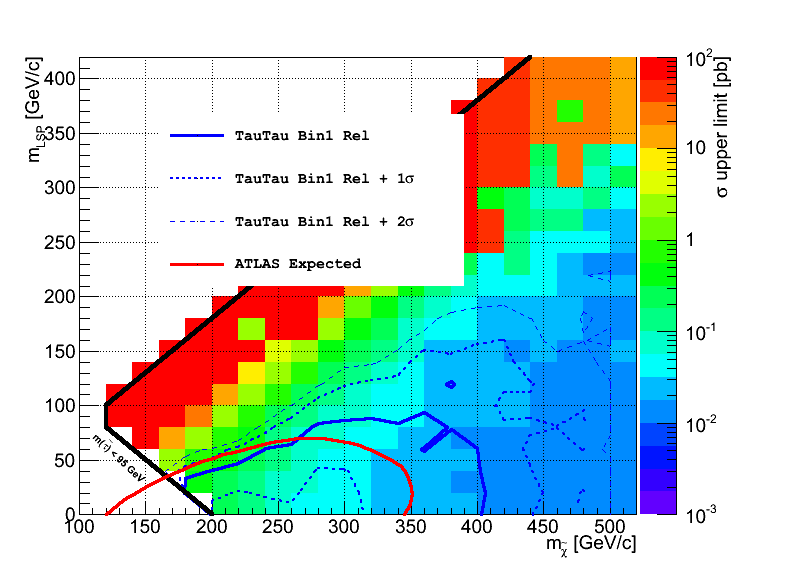
\includegraphics[width=0.49\textwidth,keepaspectratio=true]{StatisticsFig/NewFigs/TauTau_Bin1Rel.png}
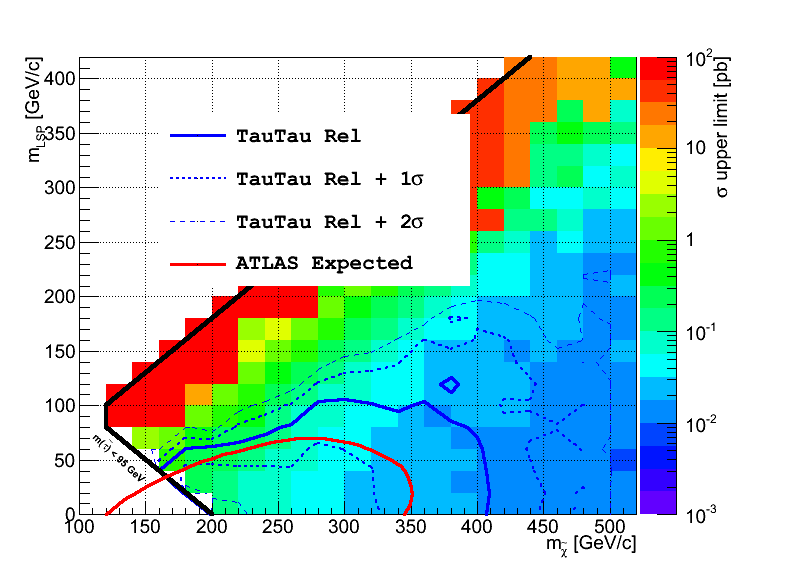
\includegraphics[width=0.49\textwidth,keepaspectratio=true]{StatisticsFig/NewFigs/TauTau_Bin1Rel_Bin2.png}
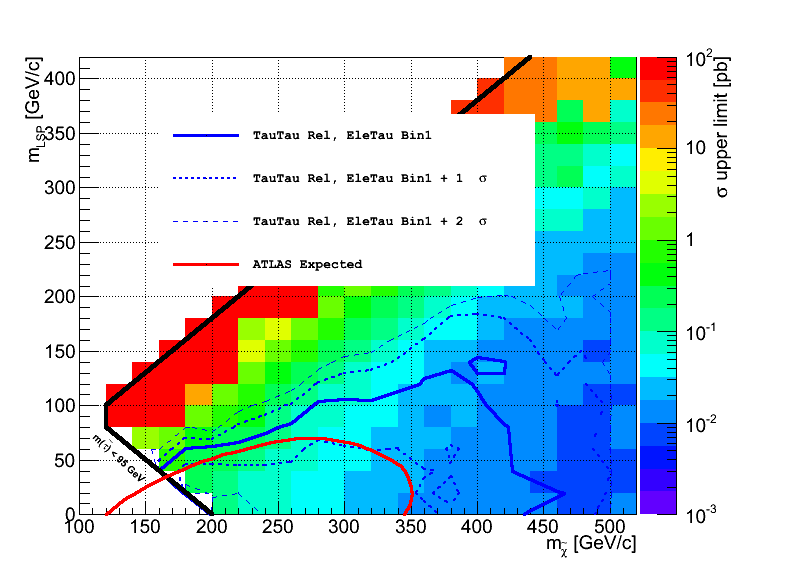
\includegraphics[width=0.49\textwidth,keepaspectratio=true]{StatisticsFig/NewFigs/TauTau_EleTauBin1.png}
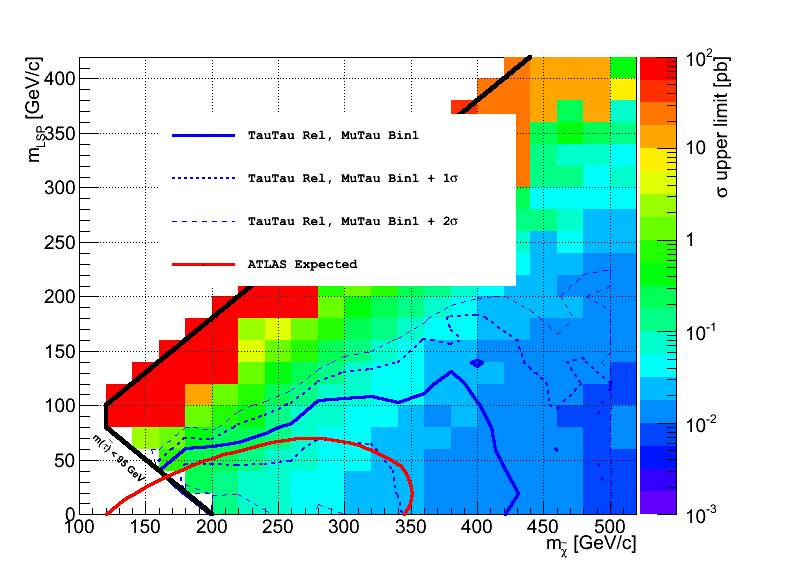
\includegraphics[width=0.49\textwidth,keepaspectratio=true]{StatisticsFig/NewFigs/TauTau_MuTauBin1.png}
\caption{These figures show the impact of each bin on the final combination. 
The top panels are related to the $\tau_{had}-\tau_{had}~$ channel including the bin 1 alone (left) and combination of bins 1 and 2 (right).
The bottom ones show the expected exclusion limit when $e-\tau_{had}~$ (left) and $\mu-\tau_{had}~$ (right) channels are included in the $\tau_{had}-\tau_{had}~$ channel.
}
\label{fig:limit_bins}
\end{figure}
\end{linenomath}
%%%%%%%%%%


Figure \ref{fig:limit_final} shows the expected upper limit on the cross section of the chargino pair production in terms of Simplified Models. 
The signal rates for each bin are 0.5420, 1.7200, 1.5800 and 0.7680, 
while overall background rates are 3.01, 1.5, 2.7 and 1.06 respectively.
However, backgrounds are taken into account in two categories, including Monte-Carlo-Driven (MCD), Data-Driven (DD).
Due to the method of background estimation in the $\tau_{had}-\tau_{had}~$ channel, bins 1 and 2 have a more category called W-jets (W).    
MCD backgrounds are feed to the package as a Gamma distribution with the corresponding statistical weights for each bin.
Furthermore, 25\% systematic uncertainity on MCD backgrounds is also considered.
All systematics are taken through LogNormal distributions.
Systematic uncertainities for each bin of DD backgrounds are 15\%, 11\%, 50\% and 69\% respectively. (numbers must be corrected)  
W backgronds have 37\% and 45\% systematic uncertainity for the first and second bins respectively.
And finally, 20\% systematic uncertainity on signal yields is considered. 
Calculation of the expected exclusion limit shows that the research has potential to exclude 
%excludes 
a sizable region of the phase space, surrounded by the lines of $m_{\PSGcpmDo} = 500\GeV$ and $m_{\PSGczDo} = 150\GeV$ with an integrated luminosity of $19.6\,\fbinv$.
The Red curve represents the expected reach by ATLAS %\cite{cutandcountAN}
 search. As the figure shows our analysis (the blue solid curve) improves the ATLAS result in the $m_{\PSGcpmDo}-m_{\PSGczDo}$ plane.

%%%%%%%%%%
\begin{linenomath}
\begin{figure}[h]
\centering
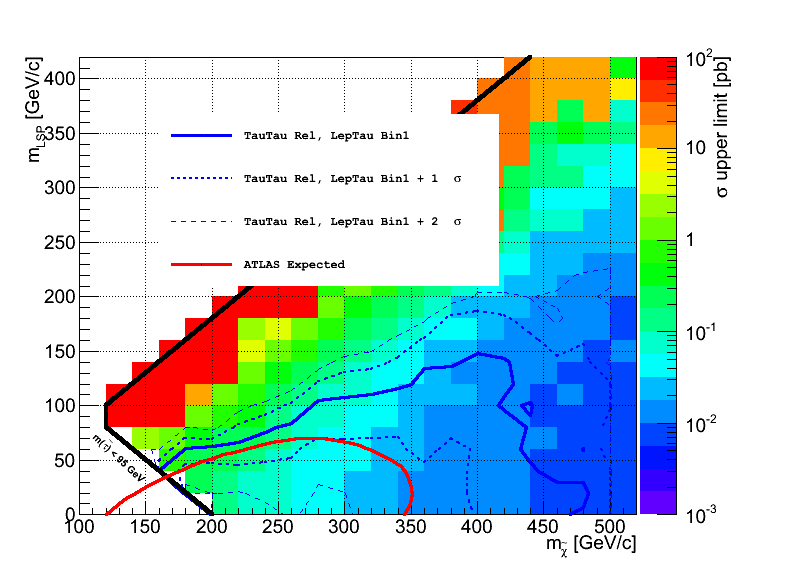
\includegraphics[width=0.7\textwidth,keepaspectratio=true]{StatisticsFig/NewFigs/Final_4BinRel.png}
\caption{Expected exclusion power in terms of Simplified Models %(T2tt-topology) 
with an integrated luminosity of $20\,\fbinv$. Backgrounds are predicted using Monte-Carlo simulations and a rough estimate of systematic uncertainties equal 
$10\%$ is taken into account.}
\label{fig:limit_final}
\end{figure}
\end{linenomath}
%%%%%%%%%%


%\rule{\textwidth}{1pt}

%In this study, we analyze data in 8 different bins (multi-bin analysis) to utilize more information from 
%the observed and the predicted distributions.
%bins' contents of the observations and the predictions.
%The bins are defined in reconstructed top quark multiplicity, zero or more. In addition, events are categorized based on the $\mttwo$ values: $125\GeV \leq \mttwo < 150\GeV,\; 150\GeV \leq \mttwo < 200\GeV,\; 200\GeV \leq \mttwo < 250\GeV,\; 250\GeV \leq \mttwo < \infty$.
%These bins are determined, for an event, based on whether the event contents reconstructed top quarks or not (2 bins) times which bin of $\mttwo$ is occupied by the event (4 bins of $125\GeV \leq \mttwo < 150\GeV,\; 150\GeV \leq \mttwo < 200\GeV,\; 200\GeV \leq \mttwo < 250\GeV,\; 250\GeV \leq \mttwo < \infty$). 

%To investigate the exclusion power of our research, we study the topology of direct stop pair production  in Simplified Models \cite{alves:sms}, with $\tilde{t}\to \PSGczDo t$ (T2tt). 
%Calculation of the expected exclusion limit shows that  
%the research has potential to exclude 
%excludes 
%a sizable region of the phase space, surrounded by the lines of $m_{\tilde{t}} = 600\GeV$ and $m_{\PSGczDo} = 175\GeV$ with an integrated luminosity of $19.6\,\fbinv$.



%Figure \ref{fig:limit_20inf} shows the expected upper limit on the cross section of the stop pair production in terms of Simplified Models. 
%Furthermore, the figure shows the expected exclusion power considering 
%$40\%$ systematic uncertainties on signal and background rates which are predicted using Monte-Carlo simulations. The black 
%dashed curve represents the expected reach by the common Cut$\&$Count \cite{cutandcountAN} search using $\MET$ trigger. 
%As the figure shows our analysis (the blue solid curve) can be comparable with other analyses and   
%it has the potential to be complementary to other analyses in some regions of the phase space.  



%%%%%%%%%%
%\begin{linenomath}
%\begin{figure}[h]
%\centering
%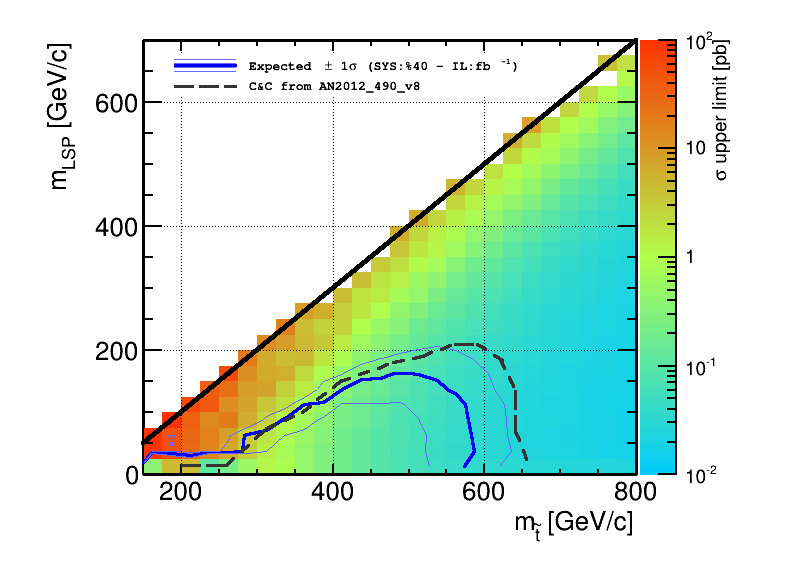
\includegraphics[width=0.9\textwidth,keepaspectratio=true]{StatisticsFig/Exc_131030_196ifb.png}
%\caption{Expected exclusion power in terms of Simplified Models (T2tt-topology) with an integrated luminosity of $20\,\fbinv$. Backgrounds are predicted using Monte-Carlo simulations and a rough estimate of systematic uncertainties equal 
%$40\%$ is taken into account.}
%\label{fig:limit_20inf}
%\end{figure}
%\end{linenomath}
%%%%%%%%%%


%%%%%%%%%%
%\begin{linenomath}
%\begin{figure}[h]
%\centering
%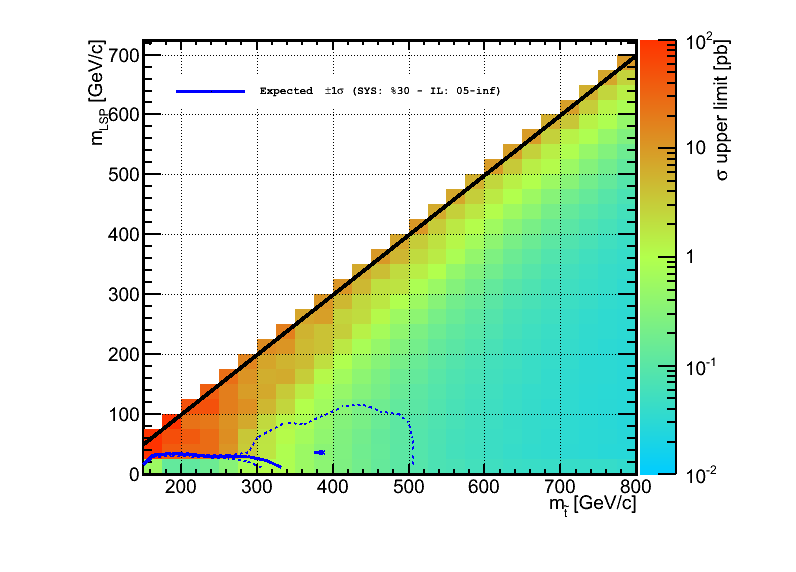
\includegraphics[width=0.7\textwidth,keepaspectratio=true]{StatisticsFig/limit_30sys_05inf_20130625.png}
%\caption{}
%\label{fig:limit_05inf}
%\end{figure}
%\end{linenomath}
%%%%%%%%%%

%%%%%%%%%%
%\begin{linenomath}
%\begin{figure}[h]
%\centering
%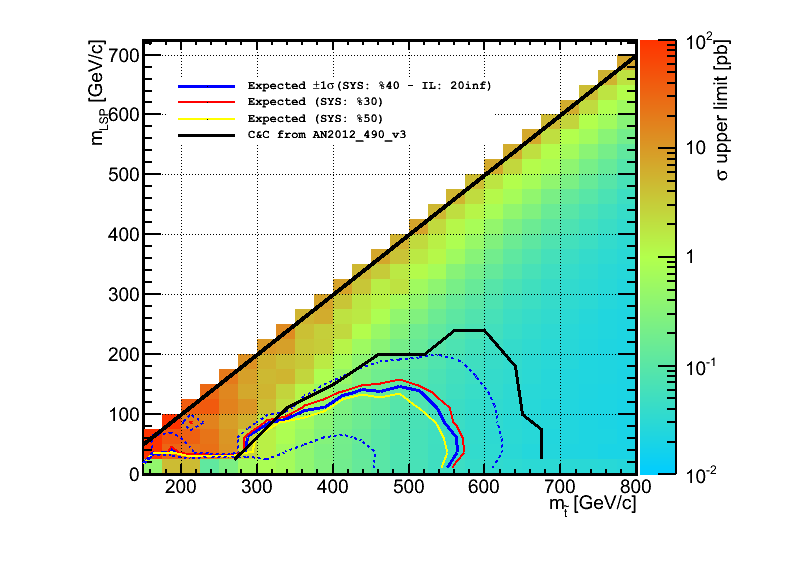
\includegraphics[width=0.7\textwidth,keepaspectratio=true]{StatisticsFig/limit_304050sys_20inf_20130625.png}
%\caption{}
%\label{fig:limit_20inf}
%\end{figure}
%\end{linenomath}
%%%%%%%%%%


\section{Conclusion}
\label{sect:conclusion}
A search for SUSY in $\tau\tau$ final state is presented. The $\tau$ pair is produced in a cascade from the production of the \PSGcpDo pair.
Different channels and search bins are introduced to increase the sensitivity to different parts of the phase space. 
Backgrounds and their systematics are discussed in details. The expected exclusion limits are also presented for different combination of the 
channels.

\section{Acknowledgments}
This analysis benefits highly from the computing resources of T2 at UCSD and codes developed in ETHZurich. 
We appreciate their help and generosity.
The authors would like to thank the previous and current conveners of the SUSY and SUSY-TBT working group, Frank Wuerthwein, Keith Ulmer, Filip Moortgat, Joshua Thompson, Pieter Everaerts and Boris Mangano for their help and support. 
The authors would like to thank the management and staff of the school of particles 
and accelerators of IPM, especially Prof. Arfaei for their help and support. 
We had several discussions with our colleagues at LIP, Pedram Bargassa, Michele Gallinaro and Cristovao Beirao Da Cruz E Silva. 
We would like to thank them for their helps and suggestions.
Thanks to all of the members of
the CMS collaboration for their outstanding results discussed partly here.

\bibliography{auto_generated}
%%% DO NOT ADD \end{document}!

